% Options for packages loaded elsewhere
\PassOptionsToPackage{unicode}{hyperref}
\PassOptionsToPackage{hyphens}{url}
\PassOptionsToPackage{dvipsnames,svgnames,x11names}{xcolor}
%
\documentclass[
  letterpaper,
  DIV=11,
  numbers=noendperiod]{scrreprt}

\usepackage{amsmath,amssymb}
\usepackage{iftex}
\ifPDFTeX
  \usepackage[T1]{fontenc}
  \usepackage[utf8]{inputenc}
  \usepackage{textcomp} % provide euro and other symbols
\else % if luatex or xetex
  \usepackage{unicode-math}
  \defaultfontfeatures{Scale=MatchLowercase}
  \defaultfontfeatures[\rmfamily]{Ligatures=TeX,Scale=1}
\fi
\usepackage{lmodern}
\ifPDFTeX\else  
    % xetex/luatex font selection
\fi
% Use upquote if available, for straight quotes in verbatim environments
\IfFileExists{upquote.sty}{\usepackage{upquote}}{}
\IfFileExists{microtype.sty}{% use microtype if available
  \usepackage[]{microtype}
  \UseMicrotypeSet[protrusion]{basicmath} % disable protrusion for tt fonts
}{}
\makeatletter
\@ifundefined{KOMAClassName}{% if non-KOMA class
  \IfFileExists{parskip.sty}{%
    \usepackage{parskip}
  }{% else
    \setlength{\parindent}{0pt}
    \setlength{\parskip}{6pt plus 2pt minus 1pt}}
}{% if KOMA class
  \KOMAoptions{parskip=half}}
\makeatother
\usepackage{xcolor}
\setlength{\emergencystretch}{3em} % prevent overfull lines
\setcounter{secnumdepth}{5}
% Make \paragraph and \subparagraph free-standing
\makeatletter
\ifx\paragraph\undefined\else
  \let\oldparagraph\paragraph
  \renewcommand{\paragraph}{
    \@ifstar
      \xxxParagraphStar
      \xxxParagraphNoStar
  }
  \newcommand{\xxxParagraphStar}[1]{\oldparagraph*{#1}\mbox{}}
  \newcommand{\xxxParagraphNoStar}[1]{\oldparagraph{#1}\mbox{}}
\fi
\ifx\subparagraph\undefined\else
  \let\oldsubparagraph\subparagraph
  \renewcommand{\subparagraph}{
    \@ifstar
      \xxxSubParagraphStar
      \xxxSubParagraphNoStar
  }
  \newcommand{\xxxSubParagraphStar}[1]{\oldsubparagraph*{#1}\mbox{}}
  \newcommand{\xxxSubParagraphNoStar}[1]{\oldsubparagraph{#1}\mbox{}}
\fi
\makeatother

\usepackage{color}
\usepackage{fancyvrb}
\newcommand{\VerbBar}{|}
\newcommand{\VERB}{\Verb[commandchars=\\\{\}]}
\DefineVerbatimEnvironment{Highlighting}{Verbatim}{commandchars=\\\{\}}
% Add ',fontsize=\small' for more characters per line
\usepackage{framed}
\definecolor{shadecolor}{RGB}{241,243,245}
\newenvironment{Shaded}{\begin{snugshade}}{\end{snugshade}}
\newcommand{\AlertTok}[1]{\textcolor[rgb]{0.68,0.00,0.00}{#1}}
\newcommand{\AnnotationTok}[1]{\textcolor[rgb]{0.37,0.37,0.37}{#1}}
\newcommand{\AttributeTok}[1]{\textcolor[rgb]{0.40,0.45,0.13}{#1}}
\newcommand{\BaseNTok}[1]{\textcolor[rgb]{0.68,0.00,0.00}{#1}}
\newcommand{\BuiltInTok}[1]{\textcolor[rgb]{0.00,0.23,0.31}{#1}}
\newcommand{\CharTok}[1]{\textcolor[rgb]{0.13,0.47,0.30}{#1}}
\newcommand{\CommentTok}[1]{\textcolor[rgb]{0.37,0.37,0.37}{#1}}
\newcommand{\CommentVarTok}[1]{\textcolor[rgb]{0.37,0.37,0.37}{\textit{#1}}}
\newcommand{\ConstantTok}[1]{\textcolor[rgb]{0.56,0.35,0.01}{#1}}
\newcommand{\ControlFlowTok}[1]{\textcolor[rgb]{0.00,0.23,0.31}{\textbf{#1}}}
\newcommand{\DataTypeTok}[1]{\textcolor[rgb]{0.68,0.00,0.00}{#1}}
\newcommand{\DecValTok}[1]{\textcolor[rgb]{0.68,0.00,0.00}{#1}}
\newcommand{\DocumentationTok}[1]{\textcolor[rgb]{0.37,0.37,0.37}{\textit{#1}}}
\newcommand{\ErrorTok}[1]{\textcolor[rgb]{0.68,0.00,0.00}{#1}}
\newcommand{\ExtensionTok}[1]{\textcolor[rgb]{0.00,0.23,0.31}{#1}}
\newcommand{\FloatTok}[1]{\textcolor[rgb]{0.68,0.00,0.00}{#1}}
\newcommand{\FunctionTok}[1]{\textcolor[rgb]{0.28,0.35,0.67}{#1}}
\newcommand{\ImportTok}[1]{\textcolor[rgb]{0.00,0.46,0.62}{#1}}
\newcommand{\InformationTok}[1]{\textcolor[rgb]{0.37,0.37,0.37}{#1}}
\newcommand{\KeywordTok}[1]{\textcolor[rgb]{0.00,0.23,0.31}{\textbf{#1}}}
\newcommand{\NormalTok}[1]{\textcolor[rgb]{0.00,0.23,0.31}{#1}}
\newcommand{\OperatorTok}[1]{\textcolor[rgb]{0.37,0.37,0.37}{#1}}
\newcommand{\OtherTok}[1]{\textcolor[rgb]{0.00,0.23,0.31}{#1}}
\newcommand{\PreprocessorTok}[1]{\textcolor[rgb]{0.68,0.00,0.00}{#1}}
\newcommand{\RegionMarkerTok}[1]{\textcolor[rgb]{0.00,0.23,0.31}{#1}}
\newcommand{\SpecialCharTok}[1]{\textcolor[rgb]{0.37,0.37,0.37}{#1}}
\newcommand{\SpecialStringTok}[1]{\textcolor[rgb]{0.13,0.47,0.30}{#1}}
\newcommand{\StringTok}[1]{\textcolor[rgb]{0.13,0.47,0.30}{#1}}
\newcommand{\VariableTok}[1]{\textcolor[rgb]{0.07,0.07,0.07}{#1}}
\newcommand{\VerbatimStringTok}[1]{\textcolor[rgb]{0.13,0.47,0.30}{#1}}
\newcommand{\WarningTok}[1]{\textcolor[rgb]{0.37,0.37,0.37}{\textit{#1}}}

\providecommand{\tightlist}{%
  \setlength{\itemsep}{0pt}\setlength{\parskip}{0pt}}\usepackage{longtable,booktabs,array}
\usepackage{calc} % for calculating minipage widths
% Correct order of tables after \paragraph or \subparagraph
\usepackage{etoolbox}
\makeatletter
\patchcmd\longtable{\par}{\if@noskipsec\mbox{}\fi\par}{}{}
\makeatother
% Allow footnotes in longtable head/foot
\IfFileExists{footnotehyper.sty}{\usepackage{footnotehyper}}{\usepackage{footnote}}
\makesavenoteenv{longtable}
\usepackage{graphicx}
\makeatletter
\newsavebox\pandoc@box
\newcommand*\pandocbounded[1]{% scales image to fit in text height/width
  \sbox\pandoc@box{#1}%
  \Gscale@div\@tempa{\textheight}{\dimexpr\ht\pandoc@box+\dp\pandoc@box\relax}%
  \Gscale@div\@tempb{\linewidth}{\wd\pandoc@box}%
  \ifdim\@tempb\p@<\@tempa\p@\let\@tempa\@tempb\fi% select the smaller of both
  \ifdim\@tempa\p@<\p@\scalebox{\@tempa}{\usebox\pandoc@box}%
  \else\usebox{\pandoc@box}%
  \fi%
}
% Set default figure placement to htbp
\def\fps@figure{htbp}
\makeatother
% definitions for citeproc citations
\NewDocumentCommand\citeproctext{}{}
\NewDocumentCommand\citeproc{mm}{%
  \begingroup\def\citeproctext{#2}\cite{#1}\endgroup}
\makeatletter
 % allow citations to break across lines
 \let\@cite@ofmt\@firstofone
 % avoid brackets around text for \cite:
 \def\@biblabel#1{}
 \def\@cite#1#2{{#1\if@tempswa , #2\fi}}
\makeatother
\newlength{\cslhangindent}
\setlength{\cslhangindent}{1.5em}
\newlength{\csllabelwidth}
\setlength{\csllabelwidth}{3em}
\newenvironment{CSLReferences}[2] % #1 hanging-indent, #2 entry-spacing
 {\begin{list}{}{%
  \setlength{\itemindent}{0pt}
  \setlength{\leftmargin}{0pt}
  \setlength{\parsep}{0pt}
  % turn on hanging indent if param 1 is 1
  \ifodd #1
   \setlength{\leftmargin}{\cslhangindent}
   \setlength{\itemindent}{-1\cslhangindent}
  \fi
  % set entry spacing
  \setlength{\itemsep}{#2\baselineskip}}}
 {\end{list}}
\usepackage{calc}
\newcommand{\CSLBlock}[1]{\hfill\break\parbox[t]{\linewidth}{\strut\ignorespaces#1\strut}}
\newcommand{\CSLLeftMargin}[1]{\parbox[t]{\csllabelwidth}{\strut#1\strut}}
\newcommand{\CSLRightInline}[1]{\parbox[t]{\linewidth - \csllabelwidth}{\strut#1\strut}}
\newcommand{\CSLIndent}[1]{\hspace{\cslhangindent}#1}

\KOMAoption{captions}{tableheading}
\makeatletter
\@ifpackageloaded{tcolorbox}{}{\usepackage[skins,breakable]{tcolorbox}}
\@ifpackageloaded{fontawesome5}{}{\usepackage{fontawesome5}}
\definecolor{quarto-callout-color}{HTML}{909090}
\definecolor{quarto-callout-note-color}{HTML}{0758E5}
\definecolor{quarto-callout-important-color}{HTML}{CC1914}
\definecolor{quarto-callout-warning-color}{HTML}{EB9113}
\definecolor{quarto-callout-tip-color}{HTML}{00A047}
\definecolor{quarto-callout-caution-color}{HTML}{FC5300}
\definecolor{quarto-callout-color-frame}{HTML}{acacac}
\definecolor{quarto-callout-note-color-frame}{HTML}{4582ec}
\definecolor{quarto-callout-important-color-frame}{HTML}{d9534f}
\definecolor{quarto-callout-warning-color-frame}{HTML}{f0ad4e}
\definecolor{quarto-callout-tip-color-frame}{HTML}{02b875}
\definecolor{quarto-callout-caution-color-frame}{HTML}{fd7e14}
\makeatother
\makeatletter
\@ifpackageloaded{bookmark}{}{\usepackage{bookmark}}
\makeatother
\makeatletter
\@ifpackageloaded{caption}{}{\usepackage{caption}}
\AtBeginDocument{%
\ifdefined\contentsname
  \renewcommand*\contentsname{Table of contents}
\else
  \newcommand\contentsname{Table of contents}
\fi
\ifdefined\listfigurename
  \renewcommand*\listfigurename{List of Figures}
\else
  \newcommand\listfigurename{List of Figures}
\fi
\ifdefined\listtablename
  \renewcommand*\listtablename{List of Tables}
\else
  \newcommand\listtablename{List of Tables}
\fi
\ifdefined\figurename
  \renewcommand*\figurename{Figure}
\else
  \newcommand\figurename{Figure}
\fi
\ifdefined\tablename
  \renewcommand*\tablename{Table}
\else
  \newcommand\tablename{Table}
\fi
}
\@ifpackageloaded{float}{}{\usepackage{float}}
\floatstyle{ruled}
\@ifundefined{c@chapter}{\newfloat{codelisting}{h}{lop}}{\newfloat{codelisting}{h}{lop}[chapter]}
\floatname{codelisting}{Listing}
\newcommand*\listoflistings{\listof{codelisting}{List of Listings}}
\makeatother
\makeatletter
\makeatother
\makeatletter
\@ifpackageloaded{caption}{}{\usepackage{caption}}
\@ifpackageloaded{subcaption}{}{\usepackage{subcaption}}
\makeatother
\makeatletter
\@ifpackageloaded{fontawesome5}{}{\usepackage{fontawesome5}}
\makeatother

\usepackage{bookmark}

\IfFileExists{xurl.sty}{\usepackage{xurl}}{} % add URL line breaks if available
\urlstyle{same} % disable monospaced font for URLs
\hypersetup{
  pdftitle={Slidecrafting with Quarto},
  pdfauthor={Emil Hvitfeldt},
  colorlinks=true,
  linkcolor={blue},
  filecolor={Maroon},
  citecolor={Blue},
  urlcolor={Blue},
  pdfcreator={LaTeX via pandoc}}


\title{Slidecrafting with Quarto}
\author{Emil Hvitfeldt}
\date{2024-08-18}

\begin{document}
\maketitle

\renewcommand*\contentsname{Table of contents}
{
\hypersetup{linkcolor=}
\setcounter{tocdepth}{2}
\tableofcontents
}

\bookmarksetup{startatroot}

\chapter*{Preface}\label{preface}
\addcontentsline{toc}{chapter}{Preface}

\markboth{Preface}{Preface}

Hello! This book is about what I like to call \textbf{slidecrafting};
The art of putting together slides that are functional and aesthetically
pleasing. I will be using \href{https://quarto.org/}{quarto
presentations} throughout the whole book. Some of the advice will
transcend quarto presentations and apply to all kinds of slide
technologies, but the book is written with quarto in mind. There will
thus inherently be some overlap with quarto documentation. It is
suggested to read all the
\href{https://quarto.org/docs/presentations/revealjs/index.html}{quarto
revealjs} documentation alongside this book for optimal learning.

I think of slidecrafting as an art because of the inexact nature of many
of the decisions you will be making after all many slide decks can be
distilled down into a series of still images, each of which should be
carefully crafted.

This book will not be able to teach you everything you need, but it will
cover the parts of the process that stay constant from deck to deck, so
you can focus on the content and develop your brand/style.

\part{Theming}

\chapter{10 Minute Theme}\label{minute-theme}

This chapter will show you how to set up a fully functional theme in
about 10 minutes. The remaining chapters of this section go into much
more detail, showcasing tips and tricks along the way.

\section{What we need}\label{what-we-need}

\begin{itemize}
\tightlist
\item
  fonts
\item
  colors
\item
  sizes
\end{itemize}

adding these things alone goes a long way

\begin{itemize}
\tightlist
\item
  logo
\end{itemize}

because it is highly requited

\begin{itemize}
\tightlist
\item
  banner/header
\end{itemize}

if there is time

\section{Fonts}\label{fonts}

\section{Colors}\label{colors}

\section{Sizes}\label{sizes}

\section{Logo}\label{logo}

\section{Banners}\label{banners}

\chapter{Colors}\label{colors-1}

\section{Finding Colors}\label{finding-colors}

When finding your colors you will mainly look for 3 different types of
colors:

\begin{itemize}
\tightlist
\item
  background colors,
\item
  text colors,
\item
  contrast colors
\end{itemize}

this is a simplistic model and it will do us just fine. In general, I
think having 3-6 colors is about the right amount of colors. This
doesn't mean that you couldn't have 10 colors in your theme, but that
you should be very deliberate in your choices.

For a small color theme, you would want a light and dark color for the
background and text color. Dark text on a light background, or light
text on dark background. Lastly, you pick a contrast color, something
that looks good with both your background and text color.

This is what you get with the default themes that are provided in
Quarto, and you can see them here in this gif:

This is also a perfect place to start looking for inspiration. using
these themes with one or two modifications might get you all the way
where you want to go. It is in general a good idea to look for
inspiration in other people's work.

Another personal favorite place of mine to go color theme hunting is on
\href{https://www.pinterest.com/}{pinterest}. I do a google search for
``Pinterest color palettes'' and go wild.

If you have any specific ideas in mind you can expand your search to
include words like ``sea'', ``beach'', ``Halloween'', or ``pastel''.

The main thing you need to keep in mind, and the biggest difference from
other types of colors you may have worked with, such as in data
visualization, is that you need to have \textbf{high contrast} between
your colors. This is by far the most important thing that separates a
good theme from a bad theme. The goal for your slides is for other
people to see them, if your contrast is low then people can't.

There are many color contrast checking websites out there, I like the
\url{https://colourcontrast.cc/} and
\href{https://coolors.co/contrast-checker/580b3a-f8f8f8}{Color Contrast
Checker by Coolors}. If possible I try to have a contrast of at least
12, but something like 10 will be okay from time to time. Which is quite
a high contrast without being impossible to hit.

\pandocbounded{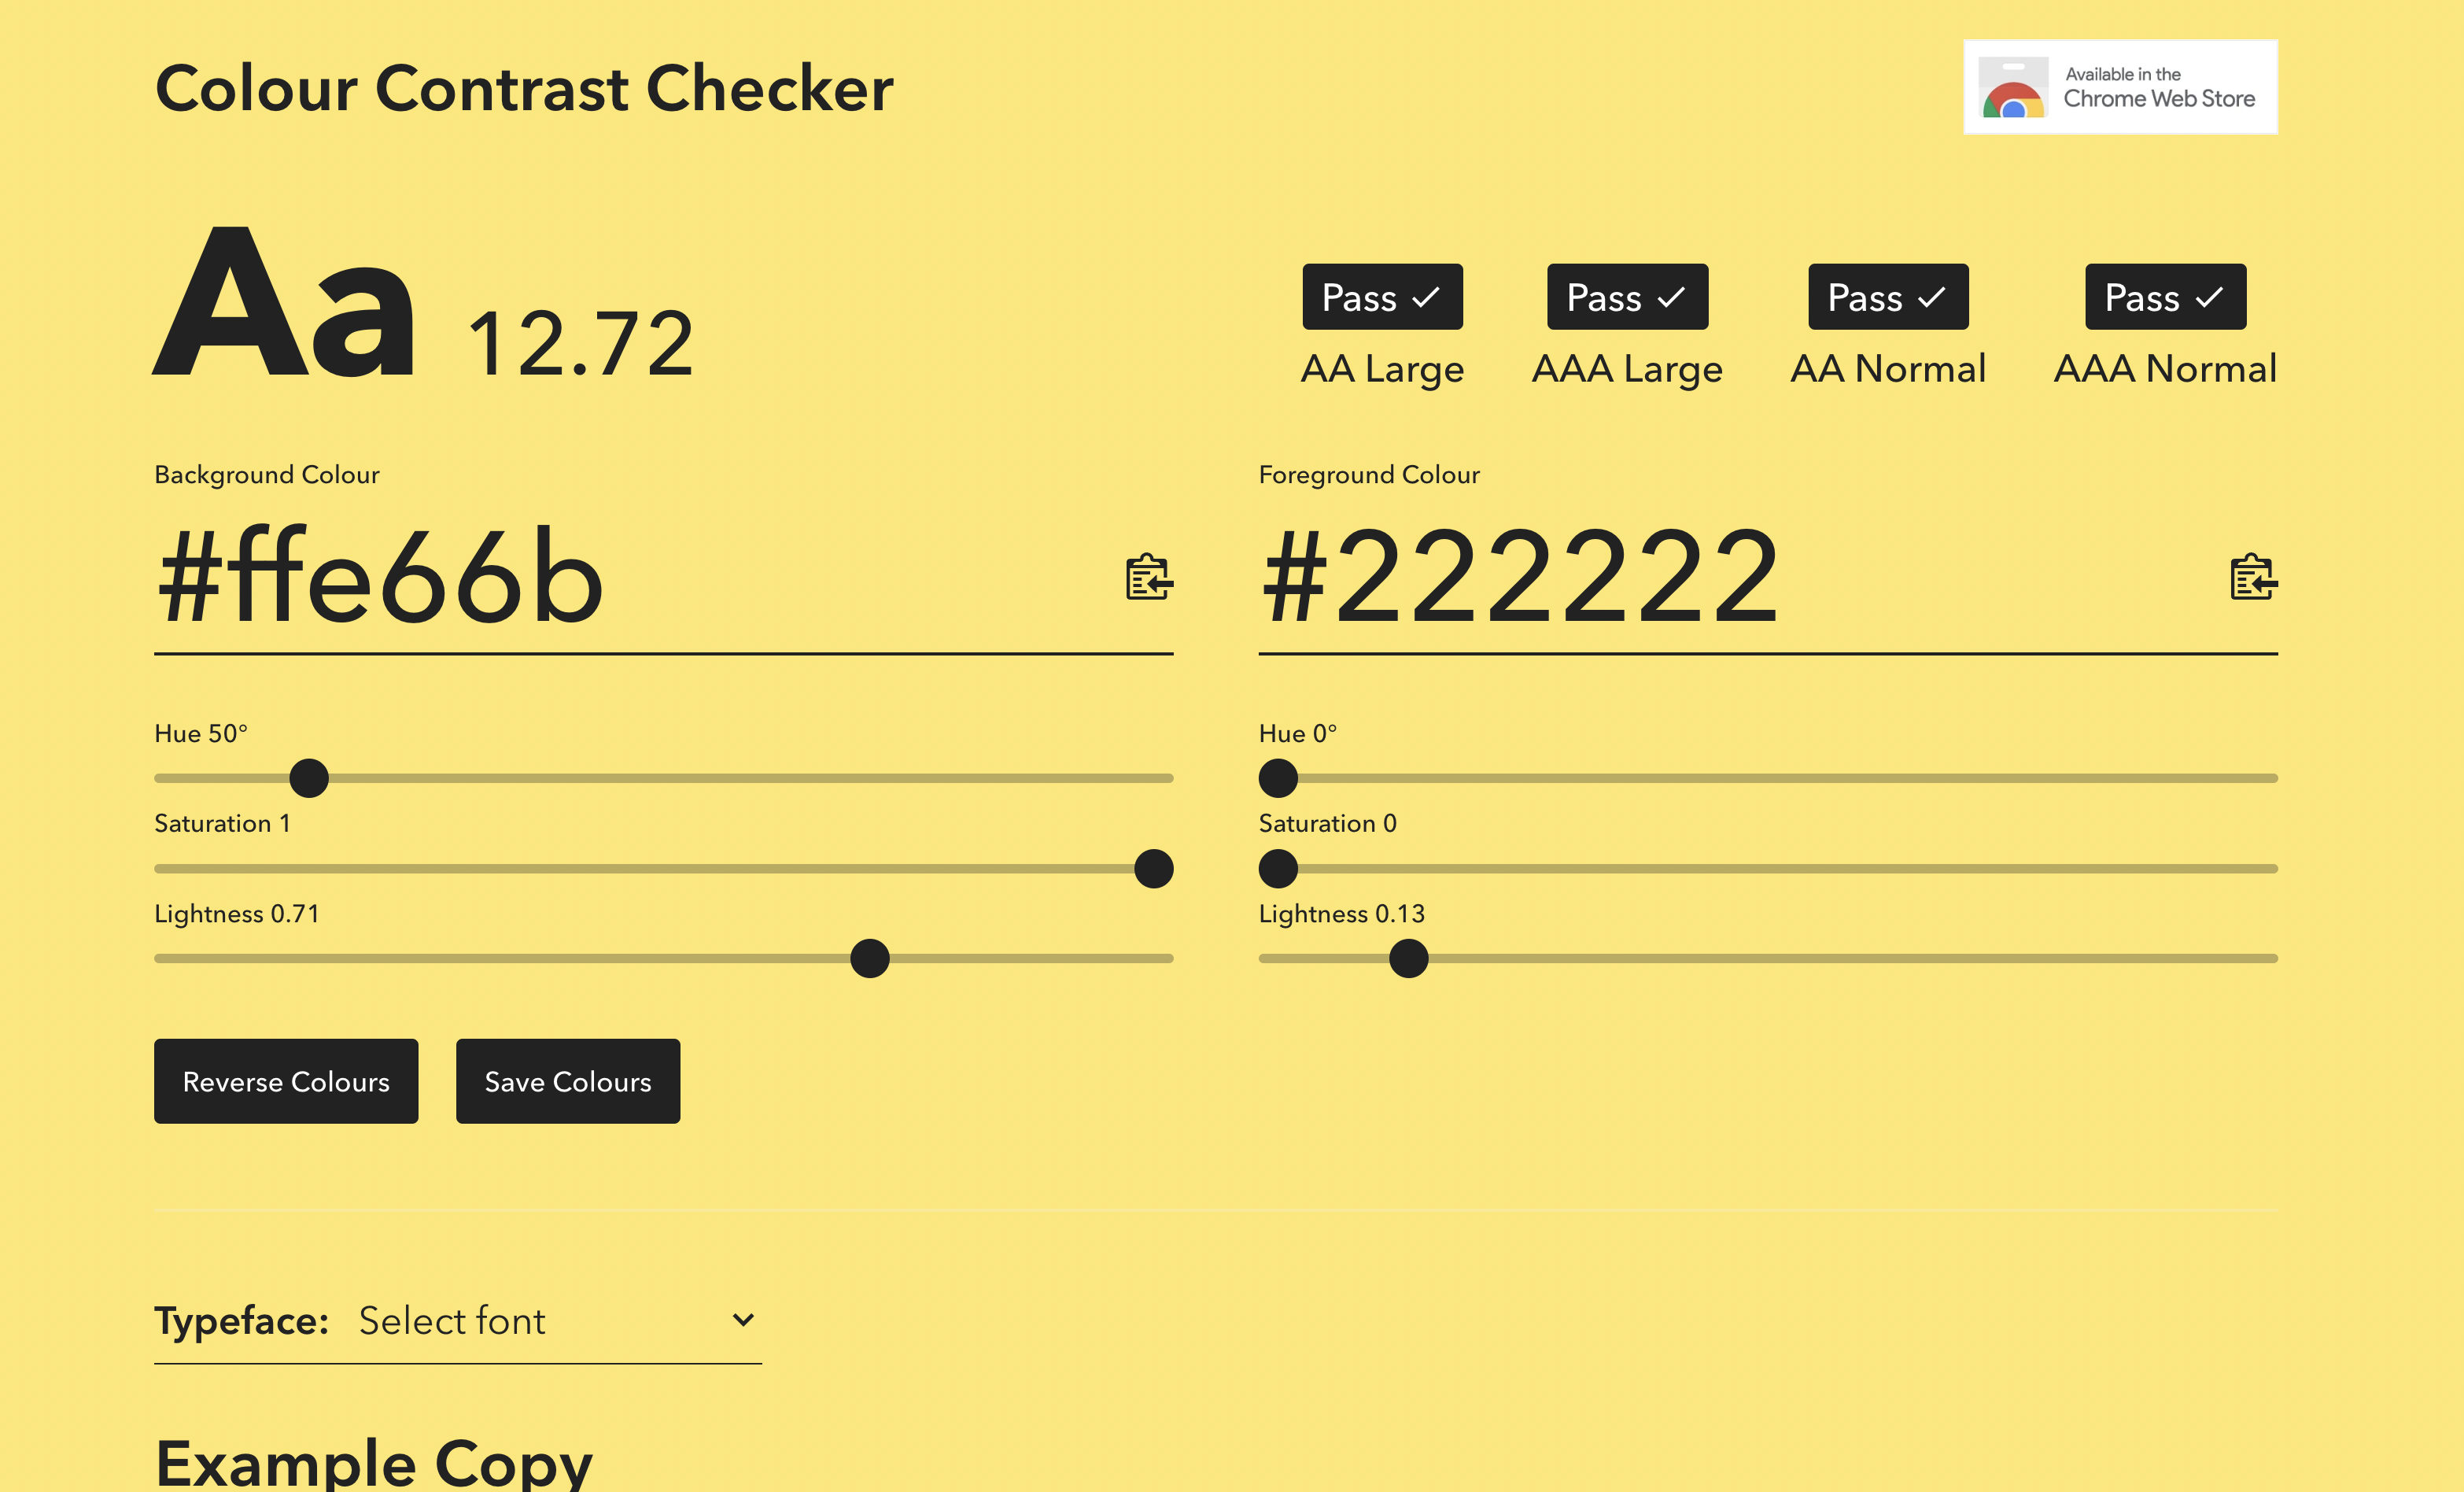
\includegraphics[keepaspectratio]{media/contrast.png}}

This contrast requirement means that both your background and text color
will be quite dark and light, as it is quite hard for most highly
saturated colors to have high contrasts to anything else.

\begin{tcolorbox}[enhanced jigsaw, titlerule=0mm, bottomrule=.15mm, opacityback=0, colbacktitle=quarto-callout-warning-color!10!white, colframe=quarto-callout-warning-color-frame, coltitle=black, breakable, toprule=.15mm, colback=white, bottomtitle=1mm, title=\textcolor{quarto-callout-warning-color}{\faExclamationTriangle}\hspace{0.5em}{Warning}, toptitle=1mm, arc=.35mm, left=2mm, leftrule=.75mm, rightrule=.15mm, opacitybacktitle=0.6]

You should try to avoid pure black and pure white. These colors can be a
bit much and can be unpleasant to look at for long periods of time.

\end{tcolorbox}

This contrast is related to font size, the smaller and finer the text
is, the more important it is that you have good contrast.

Next, we take a look at \textbf{highlight} colors! This is my term for
the colors you use to add some pop and to direct the viewers' eyes.
These colors are used for anything from link colors, highlighting,
buttons, and artistic elements.

you generally want 1 to 3 of these colors. Having at least 1 is
perfectly sufficient and you can use it to great effect to direct the
colors. 3 colors are where I'm still comfortable that they don't get
diluted. Using too many highlighting colors can confuse your viewers.

These colors should be different enough from the background and text
color that they stand out. If you are using multiple highlighting colors
you should make sure that they are colorblind-friendly with each other.
I like to use the \texttt{check\_color\_blindness()} function from the
\href{https://emilhvitfeldt.github.io/prismatic/}{prismatic} package.

\pandocbounded{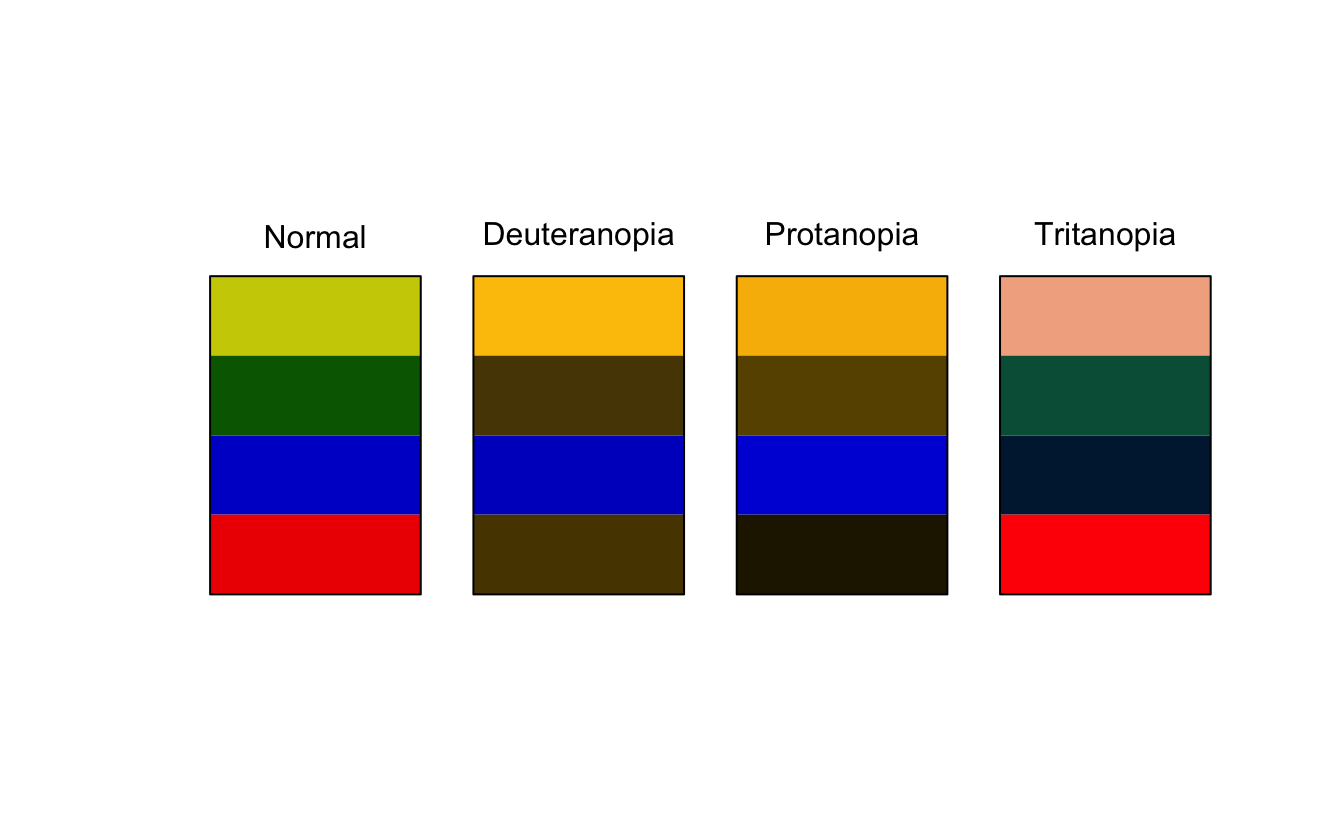
\includegraphics[keepaspectratio]{media/index_files/figure-html/unnamed-chunk-1-1.png}}

As we see above, the green and red colors don't work well together
because they are almost identical for people with Deuteranopia.

To recap:

\begin{itemize}
\tightlist
\item
  I think of or search for a palette I like
\item
  I pull out 1-2 background colors, 1-2 text colors, and 1-3 highlight
  colors
\item
  I use my color contrast checkers to validate and possibly modify my
  colors so that they are within range
\item
  I check that the colors I have are colorblind-friendly
\item
  \ldots{}
\item
  Done!
\end{itemize}

As long as I can keep the searching under 10 minutes the whole theme
creation doesn't take more than 15 minutes.

\section{Applying Colors}\label{applying-colors}

Let us try all of that in practice. I found this nice
\href{https://www.pinterest.com/pin/281123201723784541/}{blue and
yellow} color palette on Pinterest.

\pandocbounded{
\includegraphics[keepaspectratio]{media/example-theme.jpeg}}

using a color picking tool, I love
\href{https://colorslurp.com/}{ColorSlurp} I can extract the colors to
be

\begin{Shaded}
\begin{Highlighting}[]
\SpecialCharTok{*}\NormalTok{Orient}\SpecialCharTok{*}
\DecValTok{02577}\NormalTok{B}

\SpecialCharTok{*}\NormalTok{Fountain Blue}\SpecialCharTok{*}
\DecValTok{5}\NormalTok{CB4C2}

\SpecialCharTok{*}\NormalTok{Morning Glory}\SpecialCharTok{*}
\DecValTok{99}\NormalTok{D9DD}

\SpecialCharTok{*}\NormalTok{Mystic}\SpecialCharTok{*}
\NormalTok{E1E8EB}

\SpecialCharTok{*}\NormalTok{Selective Yellow}\SpecialCharTok{*}
\NormalTok{F4BA02}
\end{Highlighting}
\end{Shaded}

I'm thinking I want to use dark blue as my background colors, and the
lightest color as my text color. Before I do any modification I get the
following

\pandocbounded{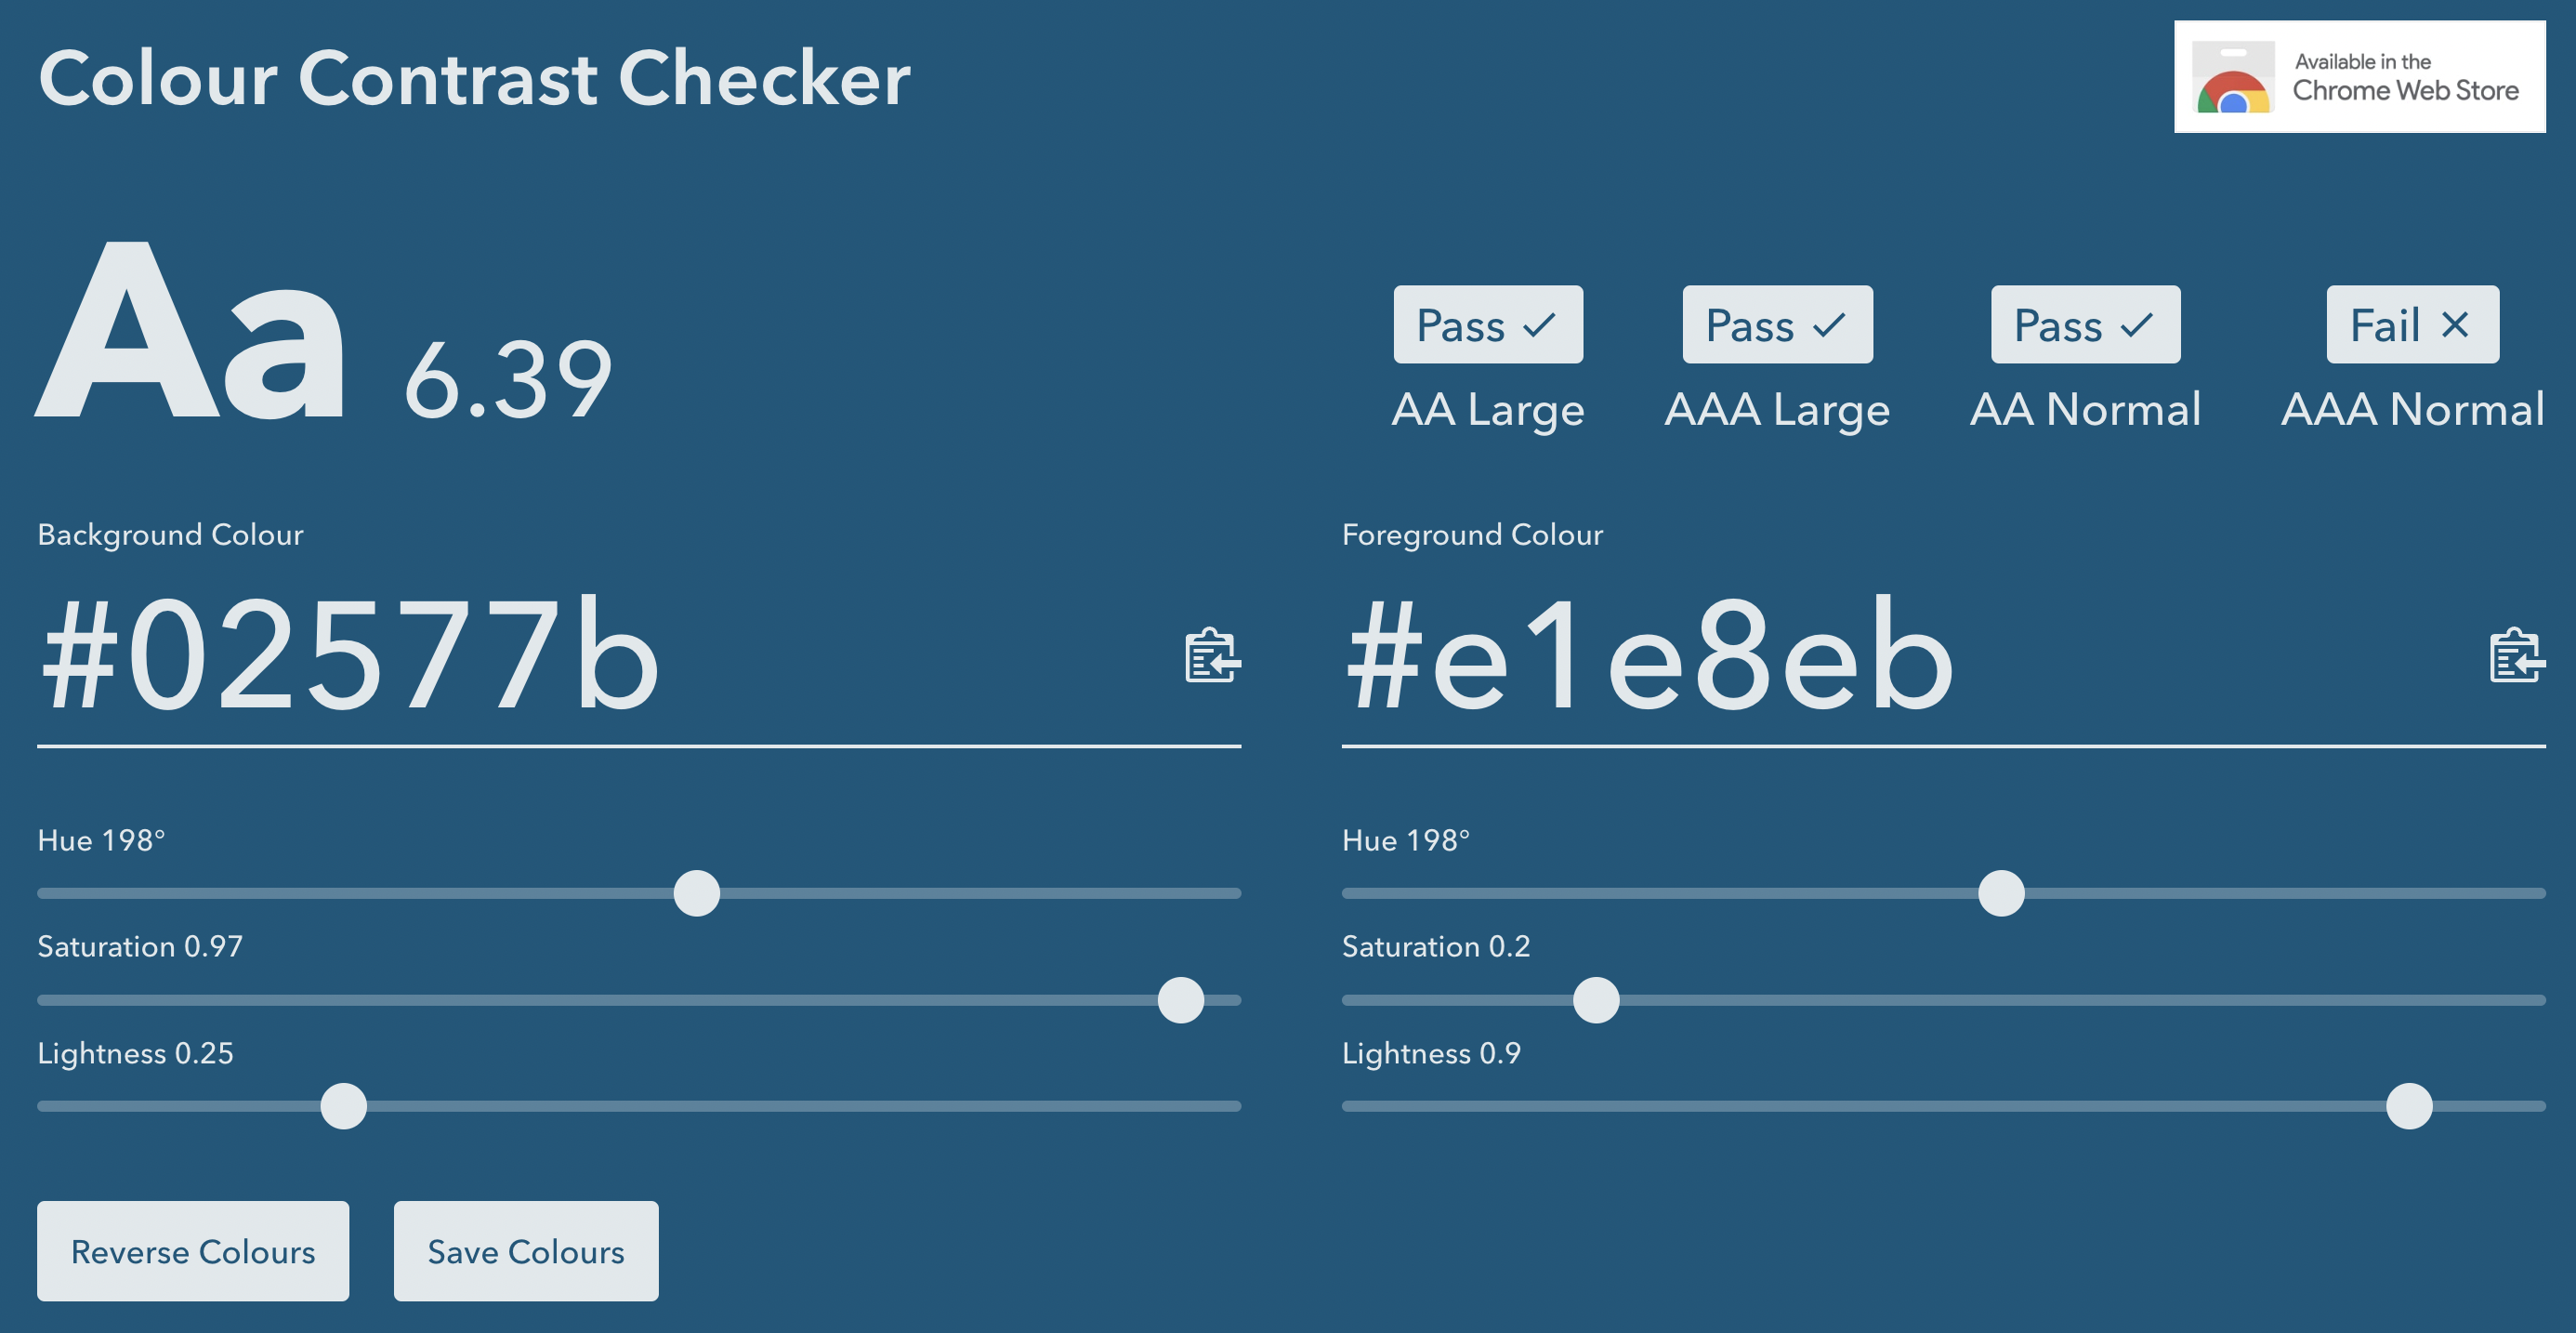
\includegraphics[keepaspectratio]{media/theme-before.png}}

And by playing the sliders a little bit I have a contrast and some
colors I'm happy with

\pandocbounded{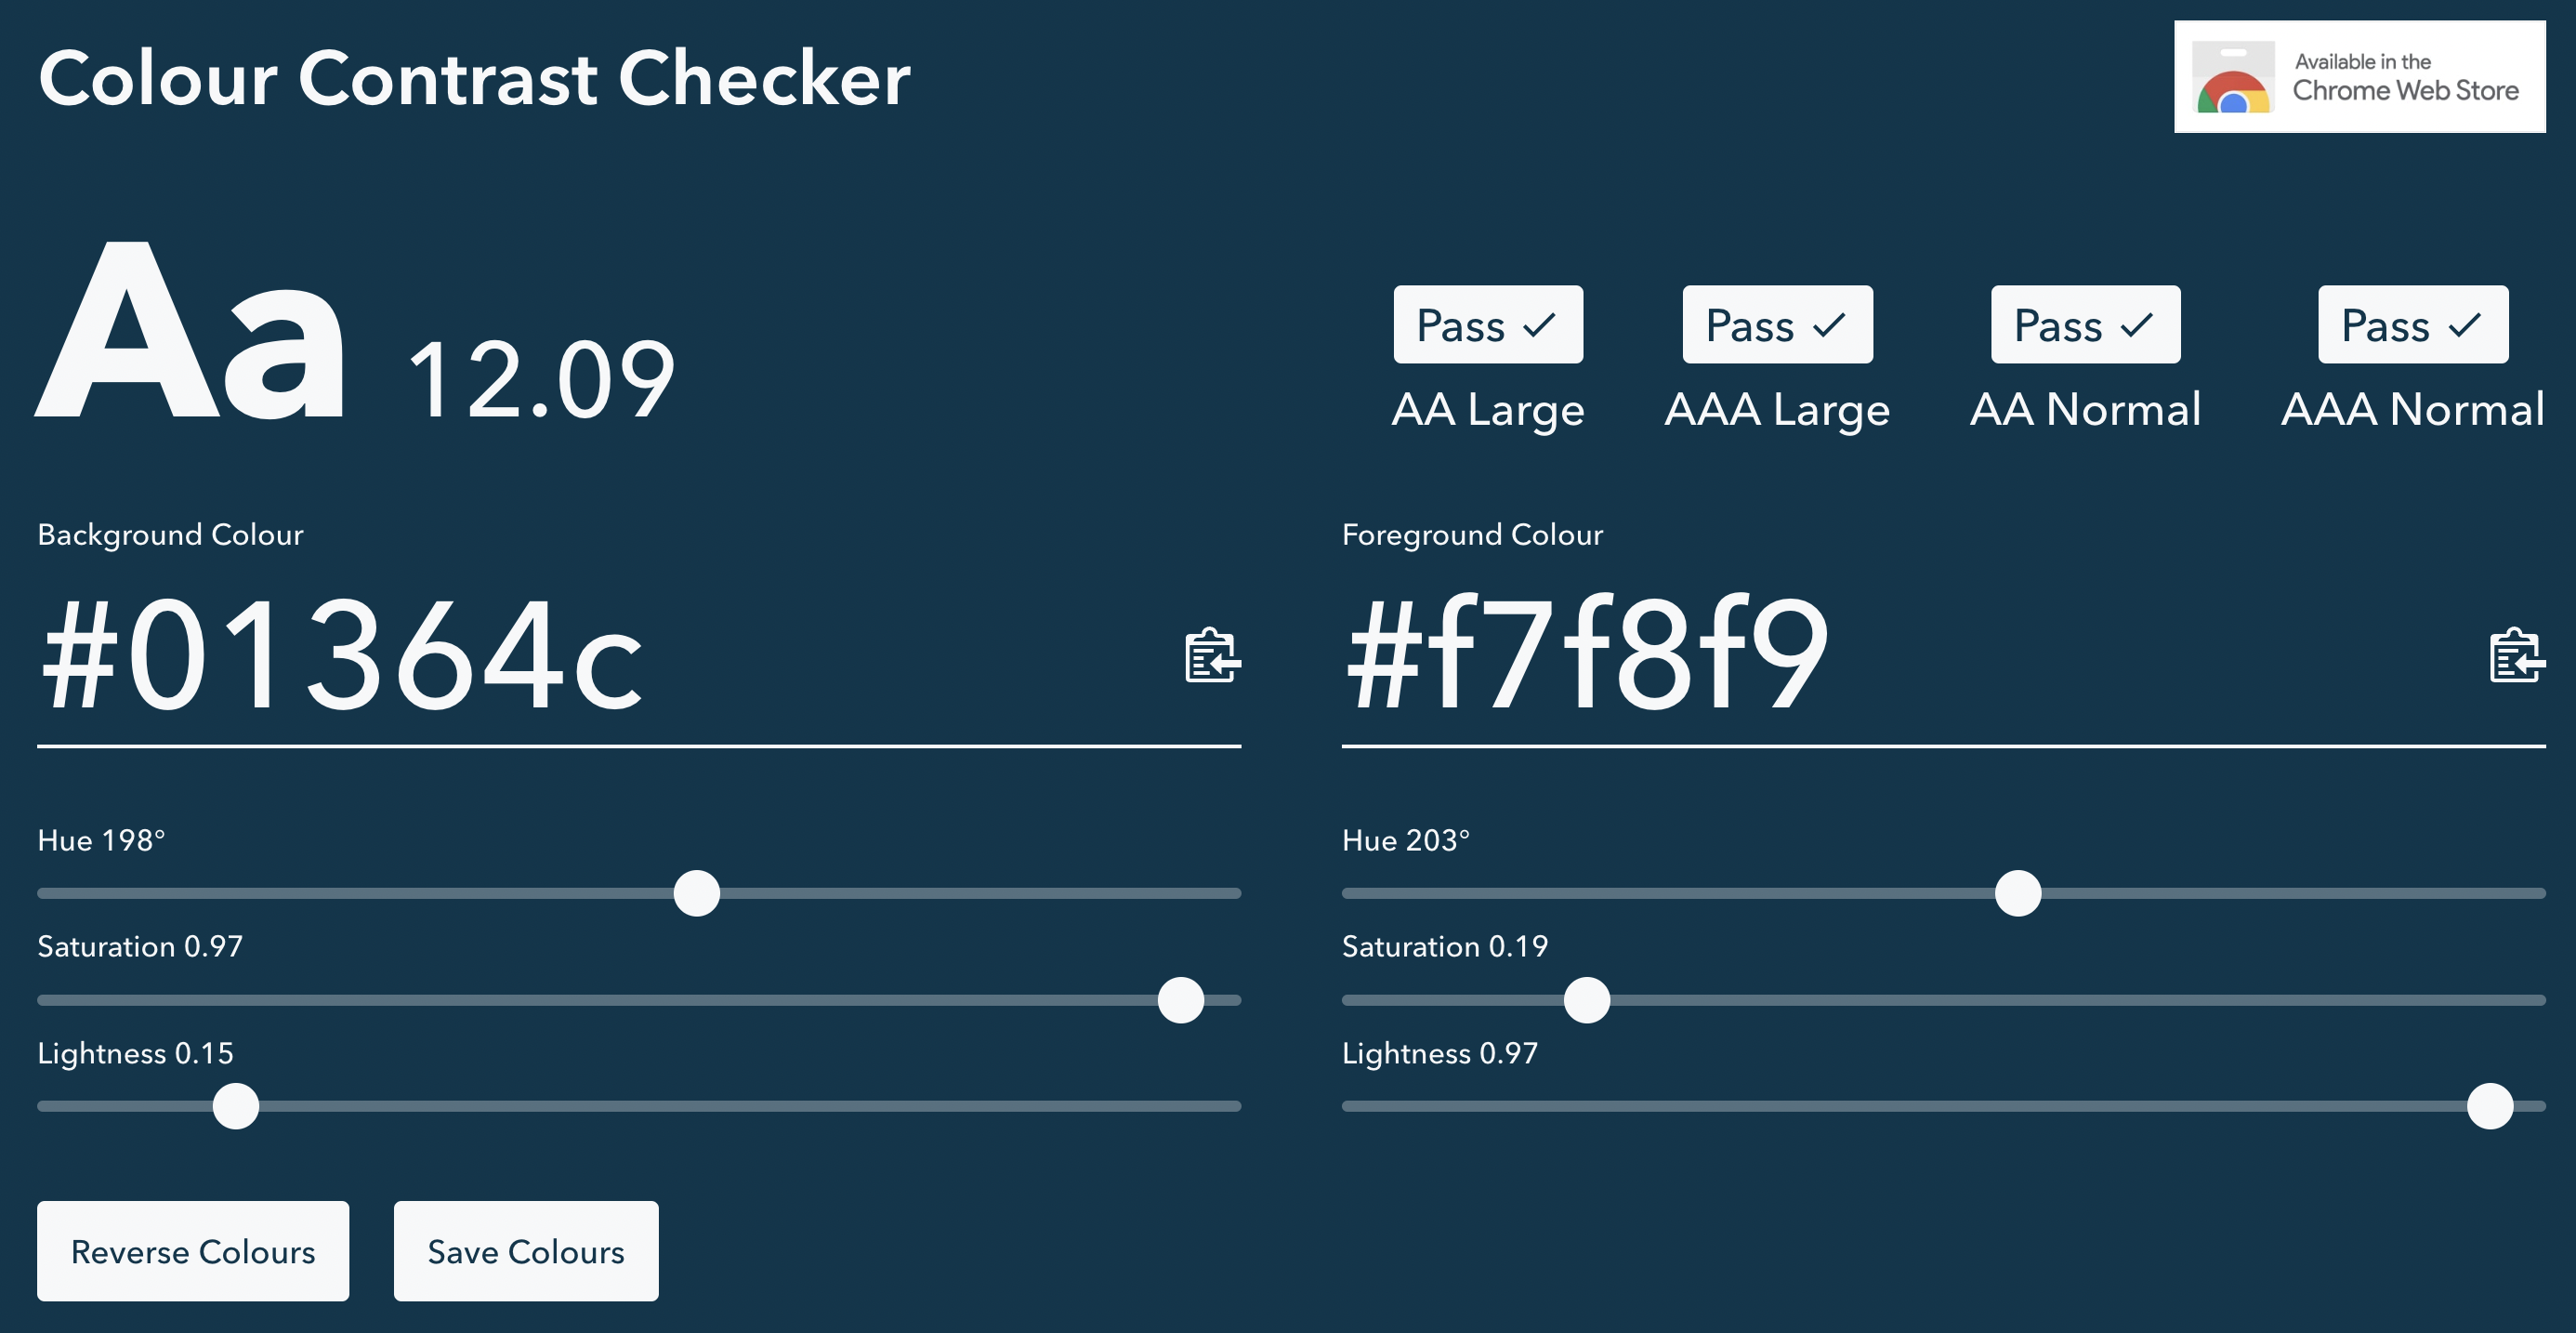
\includegraphics[keepaspectratio]{media/theme-after.png}}

We now open up our \texttt{.scss} file and fill in a couple of values.
Many of the colorings are done by relations, so we can get a lot done by
setting \texttt{\$body-bg}, \texttt{\$body-color}, and
\texttt{\$link-color}. This needs to be done inside
\texttt{scss:defaults}.

\begin{Shaded}
\begin{Highlighting}[]
\CommentTok{/*{-}{-} scss:defaults {-}{-}*/}
\VariableTok{$body{-}bg}\NormalTok{: }\ConstantTok{\#01364C}\OperatorTok{;}
\VariableTok{$body{-}color}\NormalTok{: }\ConstantTok{\#F7F8F9}\OperatorTok{;}
\VariableTok{$link{-}color}\NormalTok{: }\ConstantTok{\#99D9DD}\OperatorTok{;}

\CommentTok{/*{-}{-} scss:rules {-}{-}*/}
\end{Highlighting}
\end{Shaded}

While the above configurations are perfectly fine, I find that using
\href{https://quarto.org/docs/presentations/revealjs/themes.html\#creating-themes}{sass}
\href{https://sass-lang.com/documentation/variables}{variables} to be
clear, and it helps us tremendously if we start making more changes. So
I create variables all with the prefix \texttt{theme-} and descriptive
names so I know what is what.

\begin{Shaded}
\begin{Highlighting}[]
\CommentTok{/*{-}{-} scss:defaults {-}{-}*/}
\VariableTok{$theme{-}darkblue}\NormalTok{: }\ConstantTok{\#01364C}\OperatorTok{;}
\VariableTok{$theme{-}blue}\NormalTok{: }\ConstantTok{\#99D9DD}\OperatorTok{;}
\VariableTok{$theme{-}white}\NormalTok{: }\ConstantTok{\#F7F8F9}\OperatorTok{;}
\VariableTok{$theme{-}yellow}\NormalTok{: }\ConstantTok{\#F4BA02}\OperatorTok{;}

\VariableTok{$body{-}bg}\NormalTok{: }\VariableTok{$theme{-}darkblue}\OperatorTok{;}
\VariableTok{$body{-}color}\NormalTok{: }\VariableTok{$theme{-}white}\OperatorTok{;}
\VariableTok{$link{-}color}\NormalTok{: }\VariableTok{$theme{-}blue}\OperatorTok{;}

\CommentTok{/*{-}{-} scss:rules {-}{-}*/}
\end{Highlighting}
\end{Shaded}

This is more code, but now I can read at a glance what is happening.
This gives us the following colors on our slides. All done with minimal
code and effort. Using one of the highlight colors here to color the
links, which also affects the hamburger menu and the progress bar at the
bottom.

\pandocbounded{
\includegraphics[keepaspectratio]{media/theme-example-color.png}}

There are
\href{https://quarto.org/docs/presentations/revealjs/themes.html\#sass-variables}{several
sass variables} that are used to control how our slides look. Notice how
many of the values are defined as transformations of other values. So by
setting \texttt{\$body-bg}, \texttt{\$body-color}, and
\texttt{\$link-color} we automatically gets things like
\texttt{\$text-muted}, \texttt{\$selection-bg}, \texttt{\$border-color}
with values that works pretty well.

Let us modify our theme just a bit more before moving on to fonts. We
can use \href{https://sass-lang.com/documentation/modules/color}{sass
color functions} to modify colors based on our theme.

I want the headers to pop a little bit more, So I'm going to see if I
can make them ever so slightly lighter blue. I see that the sass
variable that controls the header color is
\texttt{\$presentation-heading-color} and that it defaults to
\texttt{\$body-color}. I use the \texttt{lighten()} function with
\texttt{\$theme-blue}, iterating a couple of times to find the perfect
value.

\begin{Shaded}
\begin{Highlighting}[]
\CommentTok{/*{-}{-} scss:defaults {-}{-}*/}
\VariableTok{$theme{-}darkblue}\NormalTok{: }\ConstantTok{\#01364C}\OperatorTok{;}
\VariableTok{$theme{-}blue}\NormalTok{: }\ConstantTok{\#99D9DD}\OperatorTok{;}
\VariableTok{$theme{-}white}\NormalTok{: }\ConstantTok{\#F7F8F9}\OperatorTok{;}
\VariableTok{$theme{-}yellow}\NormalTok{: }\ConstantTok{\#F4BA02}\OperatorTok{;}

\VariableTok{$body{-}bg}\NormalTok{: }\VariableTok{$theme{-}darkblue}\OperatorTok{;}
\VariableTok{$body{-}color}\NormalTok{: }\VariableTok{$theme{-}white}\OperatorTok{;}
\VariableTok{$link{-}color}\NormalTok{: }\VariableTok{$theme{-}blue}\OperatorTok{;}
\VariableTok{$presentation{-}heading{-}color}\NormalTok{: }\FunctionTok{lighten(}\VariableTok{$theme{-}blue}\OperatorTok{,} \DecValTok{15}\DataTypeTok{\%}\FunctionTok{)}\OperatorTok{;}

\CommentTok{/*{-}{-} scss:rules {-}{-}*/}
\end{Highlighting}
\end{Shaded}

\pandocbounded{
\includegraphics[keepaspectratio]{media/theme-example-color-header.png}}

\chapter{Fonts}\label{fonts-1}

\section{Finding Fonts}\label{finding-fonts}

We find fonts the same way we find color; using our favorites of lots of
googling. I always gravitate towards
\href{https://fonts.google.com/}{fonts.google.com}. Generally, it is
nice to use these online fonts because they are free and you don't have
to embed/ship them if you want to share your slides with others.

\pandocbounded{
\includegraphics[keepaspectratio]{media/fonts-google.png}}

Once we are in here to can search around, looking for a font you like.
For these slides, I'm going with
\href{https://fonts.google.com/specimen/Manrope}{Manrope} for the text,
and \href{https://fonts.google.com/specimen/IBM+Plex+Serif}{IBM Plex
Serif} for the headers. You must find a legible font, with a couple of
styles and bold/italics support. This is going to make your life a lot
easier once you get going.

To use ``select'' these fonts for use, you click on these links for each
font type combination.

\pandocbounded{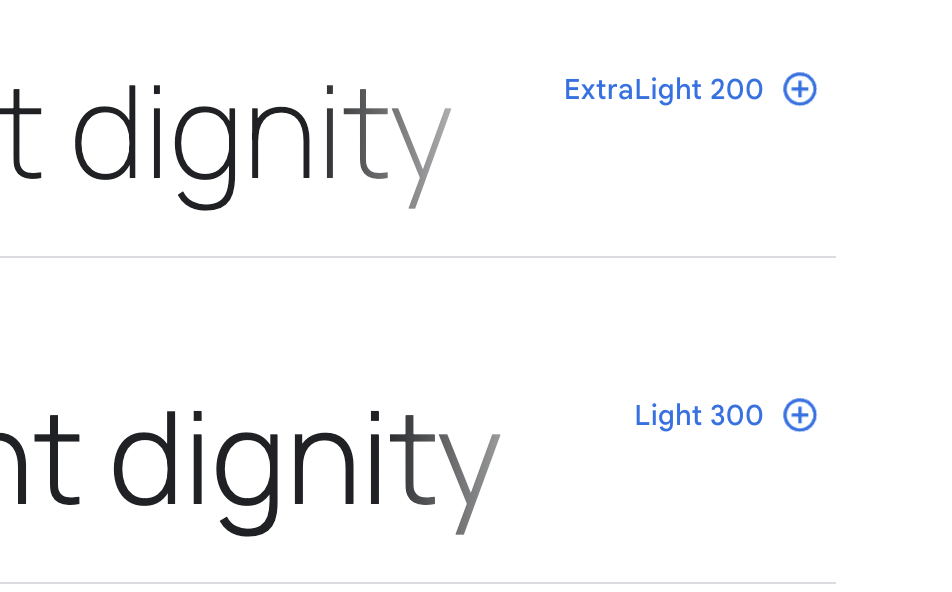
\includegraphics[keepaspectratio]{media/font-find-1.png}}

Then you click this button to have a sidebar menu pop up.

\pandocbounded{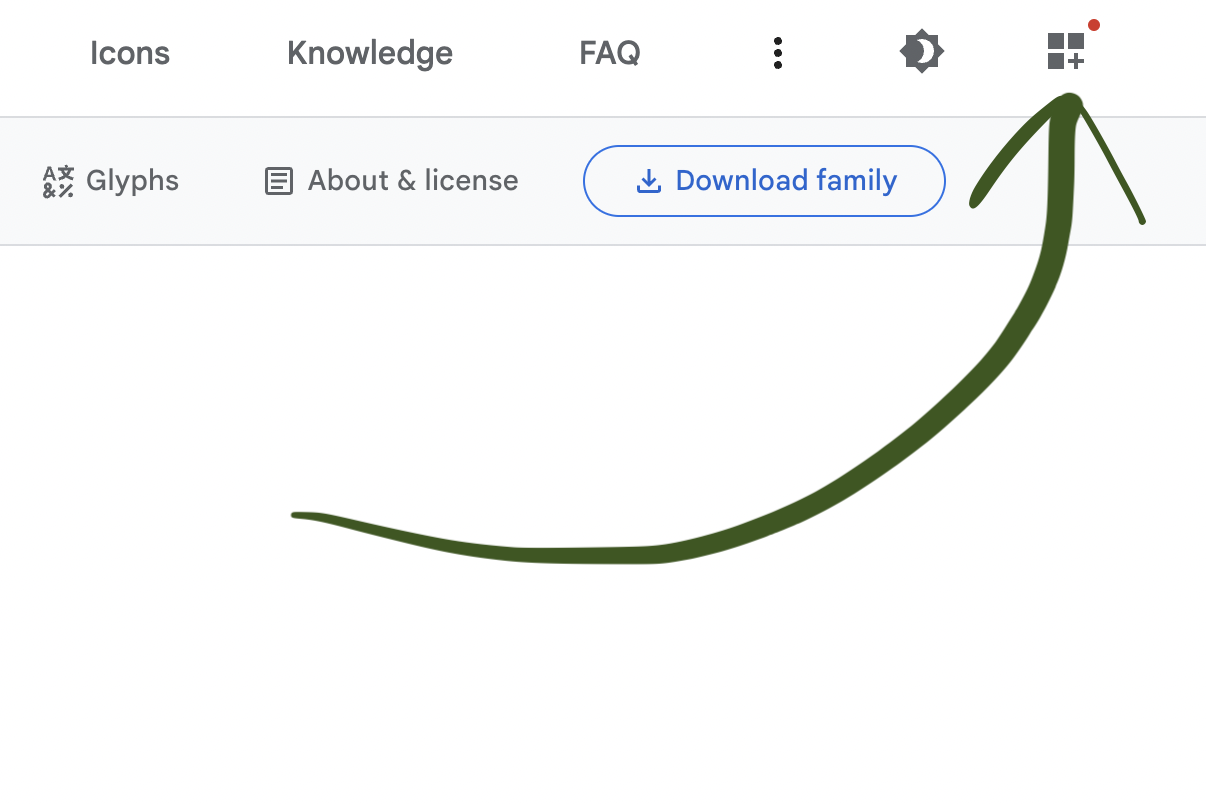
\includegraphics[keepaspectratio]{media/font-find-2.png}}

This menu lets you select and deselect the fonts you have selected. When
you are done, you can go to the ``Use on the web'' section, and click
\texttt{@import}.

\pandocbounded{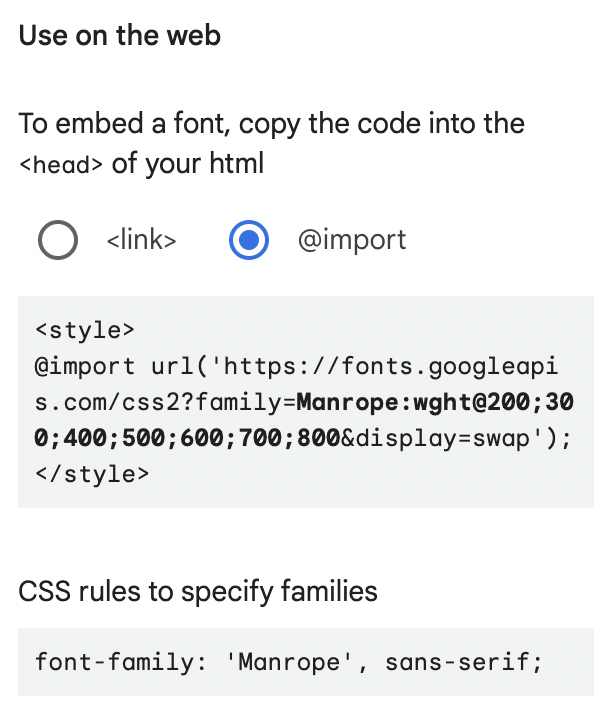
\includegraphics[keepaspectratio]{media/font-find-3.png}}

And you want to copy the code inside the
\texttt{\textless{}style\textgreater{}} tags. We are now ready to apply
these fonts to our slides!

\section{Applying Fonts}\label{applying-fonts}

Start by adding the \texttt{@import} calls we found in the previous
section. This should again go into the \texttt{scss:defaults} section of
the \texttt{.scss} file. to modify the font we have 2 sass variables.
First, we have \texttt{\$font-family-sans-serif} to modify the general
text, and \texttt{\$presentation-heading-font} to modify the headers.
Applying these changes gives us the following \texttt{.scss} file

\begin{Shaded}
\begin{Highlighting}[]
\CommentTok{/*{-}{-} scss:defaults {-}{-}*/}
\VariableTok{$theme{-}darkblue}\NormalTok{: }\ConstantTok{\#01364C}\OperatorTok{;}
\VariableTok{$theme{-}blue}\NormalTok{: }\ConstantTok{\#99D9DD}\OperatorTok{;}
\VariableTok{$theme{-}white}\NormalTok{: }\ConstantTok{\#F7F8F9}\OperatorTok{;}
\VariableTok{$theme{-}yellow}\NormalTok{: }\ConstantTok{\#F4BA02}\OperatorTok{;}

\ImportTok{@import} \FunctionTok{url(}\StringTok{\textquotesingle{}https://fonts.googleapis.com/css2?family=IBM+Plex+Serif:ital,wght@0,100;0,200;0,300;0,400;0,500;0,600;0,700;1,100;1,200;1,300;1,400;1,500;1,600;1,700\&display=swap\textquotesingle{}}\FunctionTok{)}\OperatorTok{;}
\ImportTok{@import} \FunctionTok{url(}\StringTok{\textquotesingle{}https://fonts.googleapis.com/css2?family=Manrope:wght@200;300;400;500;600;700;800\&display=swap\textquotesingle{}}\FunctionTok{)}\OperatorTok{;}

\VariableTok{$body{-}bg}\NormalTok{: }\VariableTok{$theme{-}darkblue}\OperatorTok{;}
\VariableTok{$body{-}color}\NormalTok{: }\VariableTok{$theme{-}white}\OperatorTok{;}
\VariableTok{$link{-}color}\NormalTok{: }\VariableTok{$theme{-}blue}\OperatorTok{;}
\VariableTok{$presentation{-}heading{-}color}\NormalTok{: }\FunctionTok{lighten(}\VariableTok{$theme{-}blue}\OperatorTok{,} \DecValTok{15}\DataTypeTok{\%}\FunctionTok{)}\OperatorTok{;}

\VariableTok{$font{-}family{-}sans{-}serif}\NormalTok{: }\StringTok{\textquotesingle{}Manrope\textquotesingle{}}\OperatorTok{,} \DecValTok{sans{-}serif}\OperatorTok{;}
\VariableTok{$presentation{-}heading{-}font}\NormalTok{: }\StringTok{\textquotesingle{}IBM Plex Serif\textquotesingle{}}\OperatorTok{,} \DecValTok{serif}\OperatorTok{;}

\CommentTok{/*{-}{-} scss:rules {-}{-}*/}
\end{Highlighting}
\end{Shaded}

Which when renders results in the following slides.

\pandocbounded{
\includegraphics[keepaspectratio]{media/theme-example-fonts.png}}

Notice how the fonts we used allows us to bold the words ``finished
presentation''.

Another thing you sometimes need to change depending on the font is the
sizing of the text. The sass variable
\texttt{\$presentation-font-size-root} controls this, and defaults to
\texttt{40px}. Changing this one variable will affect everything on your
slides.

You can also change the code font, this should ideally be a monospaced
font. This is done using the \texttt{\$font-family-monospace} sass
variable.

\chapter{Theme}\label{theme}

This way you can have black/white variants, white/red/blue, or any
number of different styles. If you are familiar with
\href{https://slides.yihui.org/xaringan/}{xaringan} you have seen an
\texttt{inverse} theme variant already.

\section{What is a variant?}\label{what-is-a-variant}

When we are slidecrafting, and you start having many slides. It can be
helpful to bucket them into fewer types of slides. This way you can
reuse the same style many times with minimal copy-pasting.

Using colors to create multiple variants of the same theme allows us to
quickly add similar looking, yet different styles. The \texttt{inverse}
theme variant of \{xaringan\} was a dark grey background slide, that
accompanied the white background themed default. I and many other people
found this \texttt{inverse} theme helpful for creating a break in
slides. Typically using it as a section break or a background on which
to show a quote.

You can also imagine having a couple of more similar theme variants that
are used to denote theory/practice, idea/execution, pros/cons. The
opportunities are endless, and we are not limited to only 2. I have in
the past used themes that slowly changes colors as the slides progressed
through the topics.

\section{The SCSS basics}\label{the-scss-basics}

Fortunately, adding this behavior in
\href{https://quarto.org/docs/presentations/revealjs/}{quarto revealjs}
slides. We need 2 things:

\begin{enumerate}
\def\labelenumi{\arabic{enumi}.}
\tightlist
\item
  Mark slides that have each theme variant
\item
  include css/scss to style each theme
\end{enumerate}

In our \texttt{.qmd} document we can denote each slide as a class with
the following syntax

\begin{Shaded}
\begin{Highlighting}[]
\FunctionTok{\#\# Slide}

\FunctionTok{\#\# Slide \{.variant{-}one\}}

\FunctionTok{\#\# Slide \{.variant{-}two\}}
\end{Highlighting}
\end{Shaded}

this gives the slides the corresponding \texttt{css} class which we can
create styles for. Notice how the first slide doesn't have a variant
specified. Depending on your usage, it is easier to have a good base
style, and only use \texttt{\{.class\}} to specify when you want a
different class.

create a \texttt{.scss} file and add it to the themes in the yaml
section

\begin{Shaded}
\begin{Highlighting}[]
\AnnotationTok{format:}
\NormalTok{  revealjs:}
\NormalTok{    theme: }\CommentTok{[}\OtherTok{default, styles.scss}\CommentTok{]}
\end{Highlighting}
\end{Shaded}

And in the \texttt{.scss} file, we add the boilerplate information.

\begin{Shaded}
\begin{Highlighting}[]
\CommentTok{/*{-}{-} scss:defaults {-}{-}*/}

\CommentTok{/*{-}{-} scss:rules {-}{-}*/}
\end{Highlighting}
\end{Shaded}

Under the \texttt{/*-\/-\ scss:rules\ -\/-*/} section we can now specify
all the css rules we want. And we do this by prefixing \texttt{.variant}
to each style. As an example, if we want to change the color of the text
we use \texttt{.variant-one\ \{color:\ blue;\}}, or the link color
\texttt{.variant-one\ a\ \{color:\ green;\}}.

You can quite quickly end up making many changes. And this is where I
find it helpful to use
\href{https://sass-lang.com/documentation/style-rules\#nesting}{scss
nesting}. Nesting allows us to rewrite

\begin{Shaded}
\begin{Highlighting}[]

\FunctionTok{.variant{-}one}\NormalTok{ \{}
  \KeywordTok{color}\CharTok{:} \ConstantTok{\#d6d6d6}\OperatorTok{;}
\NormalTok{\}}

\FunctionTok{.variant{-}one}\NormalTok{ h1}\OperatorTok{,}\NormalTok{ h2}\OperatorTok{,}\NormalTok{ h3 \{}
  \KeywordTok{color}\CharTok{:} \ConstantTok{\#f3f3f3}\OperatorTok{;}
\NormalTok{\}}

\FunctionTok{.variant{-}one}\NormalTok{ a \{}
  \KeywordTok{color}\CharTok{:} \ConstantTok{\#00e0e0}\OperatorTok{;}
\NormalTok{\}}

\FunctionTok{.variant{-}one}\NormalTok{ p code \{}
  \KeywordTok{color}\CharTok{:} \ConstantTok{\#ffd700}\OperatorTok{;}
\NormalTok{\}}
\end{Highlighting}
\end{Shaded}

as

\begin{Shaded}
\begin{Highlighting}[]
\FunctionTok{.variant{-}one}\NormalTok{ \{}
  \KeywordTok{color}\NormalTok{: }\ConstantTok{\#d6d6d6}\OperatorTok{;}
\NormalTok{  h1}\OperatorTok{,}\NormalTok{ h2}\OperatorTok{,}\NormalTok{ h3 \{}
    \KeywordTok{color}\NormalTok{: }\ConstantTok{\#f3f3f3}\OperatorTok{;}
\NormalTok{  \}}

\NormalTok{  a \{}
    \KeywordTok{color}\NormalTok{: }\ConstantTok{\#00e0e0}\OperatorTok{;}
\NormalTok{  \}}

\NormalTok{  p code \{}
    \KeywordTok{color}\NormalTok{: }\ConstantTok{\#ffd700}\OperatorTok{;}
\NormalTok{  \}}
\NormalTok{\}}
\end{Highlighting}
\end{Shaded}

I find it quite readable and I encourage you to follow the link and read
more about it! Using this syntax, having multiple different variants is
quite effortless, and many IDEs will help highlight and collapse this
type of syntax.

\begin{Shaded}
\begin{Highlighting}[]
\FunctionTok{.variant{-}one}\NormalTok{ \{}
  \KeywordTok{color}\NormalTok{: }\ConstantTok{\#d6d6d6}\OperatorTok{;}
\NormalTok{  h1}\OperatorTok{,}\NormalTok{ h2}\OperatorTok{,}\NormalTok{ h3 \{}
    \KeywordTok{color}\NormalTok{: }\ConstantTok{\#f3f3f3}\OperatorTok{;}
\NormalTok{  \}}

\NormalTok{  a \{}
    \KeywordTok{color}\NormalTok{: }\ConstantTok{\#00e0e0}\OperatorTok{;}
\NormalTok{  \}}

\NormalTok{  p code \{}
    \KeywordTok{color}\NormalTok{: }\ConstantTok{\#ffd700}\OperatorTok{;}
\NormalTok{  \}}
\NormalTok{\}}

\FunctionTok{.variant{-}two}\NormalTok{ \{}
  \KeywordTok{color}\NormalTok{: }\ConstantTok{\#a6a6d6}\OperatorTok{;}
\NormalTok{  h1}\OperatorTok{,}\NormalTok{ h2}\OperatorTok{,}\NormalTok{ h3 \{}
    \KeywordTok{color}\NormalTok{: }\ConstantTok{\#222222}\OperatorTok{;}
\NormalTok{  \}}

\NormalTok{  a \{}
    \KeywordTok{color}\NormalTok{: }\ConstantTok{\#f22341}\OperatorTok{;}
\NormalTok{  \}}

\NormalTok{  p code \{}
    \KeywordTok{color}\NormalTok{: }\ConstantTok{\#ff00ff}\OperatorTok{;}
\NormalTok{  \}}
\NormalTok{\}}
\end{Highlighting}
\end{Shaded}

And that is all that is needed! I have taken the liberty to create two
themes to show case how this is done in practice:

https://github.com/EmilHvitfeldt/quarto-revealjs-inverse

https://github.com/EmilHvitfeldt/quarto-revealjs-seasons

\section{What is a slide theme?}\label{what-is-a-slide-theme}

The inspiration for this style of slidecraft isn't anything new. If you
have used conventional slide-making tools you have seen a dropdown menu
before

\pandocbounded{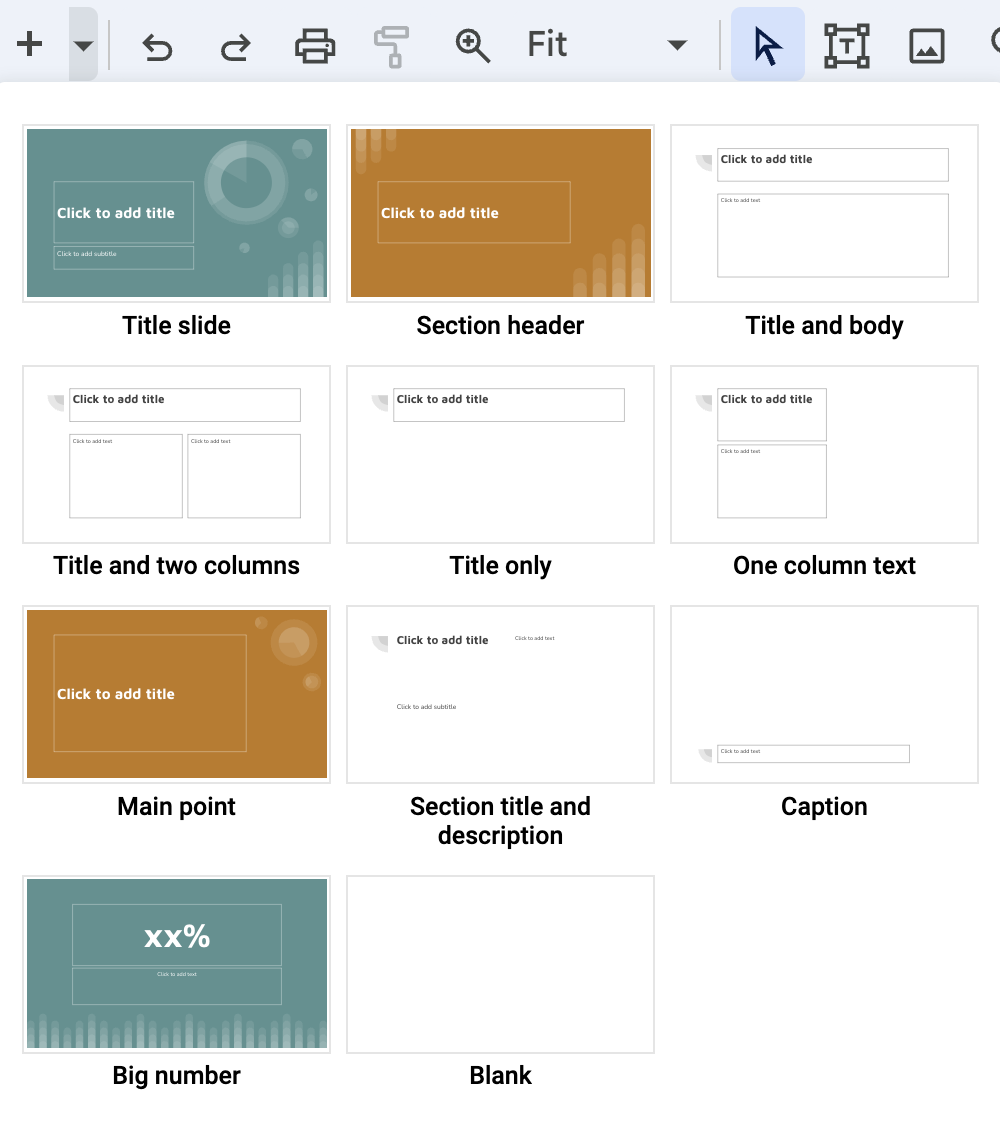
\includegraphics[keepaspectratio]{media/google-slides.png}}

With these menus, you can swiftly select the style of slide you intend
to write and fill in the content. I find that for some presentations
that I all I need.

Below is one such theme I created (it is a real revealjs slide deck,
touch and advance the slides)

\faIcon{github} Github \faIcon{door-open} Website

Instead of carefully managing the style of all the elements of each
slide. They all have an overall slide theme that controls all the
content on the slide. This controls colors and sizes but can go further
and control backgrounds and even the positioning of elements.

Take \texttt{.theme-section1} as an example. Not only are the text and
colors modified. The text region is being modified such that the text
isn't going to overlap with the globe on the right. Setting this up
beforehand is quite nice. While the backgrounds might seem complicated,
they are all SVGs, but you can use any other type of image or none at
all.

Once you have created the theme, your slides will look like this:

\begin{Shaded}
\begin{Highlighting}[]
\FunctionTok{\#\# Happy slides \{.theme{-}title1 .center\}}

\FunctionTok{\#\# Fancy Section \{.theme{-}section3 .center\}}

\FunctionTok{\#\#\# Less Fancy Subtitle}

\FunctionTok{\#\# Funny title \{.theme{-}slide1\}}

\NormalTok{Content}

\FunctionTok{\#\# Exciting title \{.theme{-}slide2\}}

\NormalTok{Content}

\FunctionTok{\#\# Sad title \{.theme{-}slide3\}}

\NormalTok{Content}
\end{Highlighting}
\end{Shaded}

Each slide will have minimal CSS, just one or two classes specified on
the slide level.

\section{How to create your own}\label{how-to-create-your-own}

We will assume that we start our project the same way as we did
\href{https://www.emilhvitfeldt.com/post/slidecraft-theme-variants/\#the-sass-basics}{in
previous blog posts}. What we will be doing is creating several
\texttt{CSS} classes. I find it easier to prefix all of them with
\texttt{.theme-} but that is not a requirement. We will also be using
the feature that
\href{https://sass-lang.com/documentation/style-rules/\#nesting}{Sass
lets us create nesting rules css}.

We start with a simple class rule

\begin{Shaded}
\begin{Highlighting}[]
\FunctionTok{.theme{-}slide1}\NormalTok{ \{}
\NormalTok{\}}
\end{Highlighting}
\end{Shaded}

if we are following my advice on
\href{https://www.emilhvitfeldt.com/post/slidecraft-colors-fonts/\#applying-colors}{creating
css color palettes} then we can use those to specify header colors

\begin{Shaded}
\begin{Highlighting}[]
\FunctionTok{.theme{-}slide1}\NormalTok{ \{}
\NormalTok{  h3 \{}
    \KeywordTok{color}\NormalTok{: }\VariableTok{$theme{-}blue}\OperatorTok{;} \CommentTok{// or \#5CB4C2}
\NormalTok{  \}}
\NormalTok{\}}
\end{Highlighting}
\end{Shaded}

And we can specify anything want in here. Note that anything inside
\texttt{h3} applies to all \texttt{h3} headers in \texttt{.theme-slide1}
slides.

\begin{Shaded}
\begin{Highlighting}[]
\FunctionTok{.theme{-}slide1}\NormalTok{ \{}
\NormalTok{  h3 \{}
    \KeywordTok{color}\NormalTok{: }\VariableTok{$theme{-}blue}\OperatorTok{;} \CommentTok{// or \#5CB4C2}
    \KeywordTok{font{-}size}\NormalTok{: }\DecValTok{2}\DataTypeTok{em}\OperatorTok{;}
\NormalTok{  \}}
\NormalTok{\}}
\end{Highlighting}
\end{Shaded}

We could specify specific background colors

\begin{Shaded}
\begin{Highlighting}[]
\FunctionTok{.theme{-}slide1}\NormalTok{ \{}
  \KeywordTok{background{-}color}\NormalTok{: }\ConstantTok{\#E1E8EB}
\NormalTok{  h3 \{}
    \KeywordTok{color}\NormalTok{: }\VariableTok{$theme{-}blue}\OperatorTok{;} \CommentTok{// or \#5CB4C2}
    \KeywordTok{font{-}size}\NormalTok{: }\DecValTok{2}\DataTypeTok{em}\OperatorTok{;}
\NormalTok{  \}}
\NormalTok{\}}
\end{Highlighting}
\end{Shaded}

Or we could specify background images, for reasons I don't want to get
into, this is the way to include an image nicely. With
\texttt{../../../../../assets/slide1.svg} being a valid path to the
slides. You may have to modify the number of \texttt{../} for this to
work

\begin{Shaded}
\begin{Highlighting}[]
\FunctionTok{.theme{-}slide1}\NormalTok{ \{}
  \OperatorTok{\&}\InformationTok{:is(.slide{-}background)}\NormalTok{ \{}
    \KeywordTok{background{-}image}\NormalTok{: }\FunctionTok{url(}\StringTok{\textquotesingle{}../../../../../assets/slide1.svg\textquotesingle{}}\FunctionTok{)}\OperatorTok{;}
    \KeywordTok{background{-}size}\NormalTok{: }\DecValTok{cover}\OperatorTok{;}
    \KeywordTok{background{-}position}\NormalTok{: }\DecValTok{center}\OperatorTok{;}
    \KeywordTok{background{-}repeat}\NormalTok{: }\DecValTok{no{-}repeat}\OperatorTok{;}
\NormalTok{  \}}
\NormalTok{  h3 \{}
    \KeywordTok{color}\NormalTok{: }\VariableTok{$theme{-}blue}\OperatorTok{;} \CommentTok{// or \#5CB4C2}
    \KeywordTok{font{-}size}\NormalTok{: }\DecValTok{2}\DataTypeTok{em}\OperatorTok{;}
\NormalTok{  \}}
\NormalTok{\}}
\end{Highlighting}
\end{Shaded}

depending on your slides you might have repeated styles a lot. Sass has
a way to help us with
\href{https://sass-lang.com/documentation/at-rules/mixin/}{\texttt{@mixin}
and \texttt{@include}}. You can create a \texttt{@mixin} with several
styles, and then instead of copying around all the styles, you can
\texttt{@include} the mixin for the same effect. Using this we now have
the following

\begin{Shaded}
\begin{Highlighting}[]
\ImportTok{@mixin} \FunctionTok{background{-}full}\NormalTok{ \{}
  \KeywordTok{background{-}size}\NormalTok{: }\DecValTok{cover}\OperatorTok{;}
  \KeywordTok{background{-}position}\NormalTok{: }\DecValTok{center}\OperatorTok{;}
  \KeywordTok{background{-}repeat}\NormalTok{: }\DecValTok{no{-}repeat}\OperatorTok{;}
\NormalTok{\}}

\FunctionTok{.theme{-}slide1}\NormalTok{ \{}
  \OperatorTok{\&}\InformationTok{:is(.slide{-}background)}\NormalTok{ \{}
    \KeywordTok{background{-}image}\NormalTok{: }\FunctionTok{url(}\StringTok{\textquotesingle{}../../../../../assets/slide1.svg\textquotesingle{}}\FunctionTok{)}\OperatorTok{;}
    \ImportTok{@include}\NormalTok{ background{-}full}\OperatorTok{;}
\NormalTok{  \}}
\NormalTok{  h3 \{}
    \KeywordTok{color}\NormalTok{: }\VariableTok{$theme{-}blue}\OperatorTok{;} \CommentTok{// or \#5CB4C2}
    \KeywordTok{font{-}size}\NormalTok{: }\DecValTok{2}\DataTypeTok{em}\OperatorTok{;}
\NormalTok{  \}}
\NormalTok{\}}
\end{Highlighting}
\end{Shaded}

Lastly, if you are using images the way I'm using them, you will need to
change the text regions to avoid text overlapping with the background
image, we can use the \texttt{margin-} rules for that

\begin{Shaded}
\begin{Highlighting}[]
\ImportTok{@mixin} \FunctionTok{background{-}full}\NormalTok{ \{}
  \KeywordTok{background{-}size}\NormalTok{: }\DecValTok{cover}\OperatorTok{;}
  \KeywordTok{background{-}position}\NormalTok{: }\DecValTok{center}\OperatorTok{;}
  \KeywordTok{background{-}repeat}\NormalTok{: }\DecValTok{no{-}repeat}\OperatorTok{;}
\NormalTok{\}}

\FunctionTok{.theme{-}slide1}\NormalTok{ \{}
  \OperatorTok{\&}\InformationTok{:is(.slide{-}background)}\NormalTok{ \{}
    \KeywordTok{background{-}image}\NormalTok{: }\FunctionTok{url(}\StringTok{\textquotesingle{}../../../../../assets/slide1.svg\textquotesingle{}}\FunctionTok{)}\OperatorTok{;}
    \ImportTok{@include}\NormalTok{ background{-}full}\OperatorTok{;}
\NormalTok{  \}}
\NormalTok{  h3 \{}
    \KeywordTok{color}\NormalTok{: }\VariableTok{$theme{-}blue}\OperatorTok{;} \CommentTok{// or \#5CB4C2}
    \KeywordTok{font{-}size}\NormalTok{: }\DecValTok{2}\DataTypeTok{em}\OperatorTok{;}
\NormalTok{  \}}
\NormalTok{  h2}\OperatorTok{,}\NormalTok{ h3}\OperatorTok{,}\NormalTok{ h4}\OperatorTok{,}\NormalTok{ h5}\OperatorTok{,}\NormalTok{ p}\OperatorTok{,}\NormalTok{ pre \{}
    \KeywordTok{margin{-}left}\NormalTok{: }\DecValTok{100}\DataTypeTok{px}\OperatorTok{;}
\NormalTok{  \}}
\NormalTok{\}}
\end{Highlighting}
\end{Shaded}

I hope you can see that with this style of slidecrafting, the skies the
limit. The style sheet for the above example can be
\href{https://github.com/EmilHvitfeldt/quarto-revealjs-earth/blob/main/_extensions/earth/earth.scss}{found
here}.

\section{More Examples}\label{more-examples}

Below is another theme, following very closely the construction of the
previous

\faIcon{github} Github \faIcon{door-open} Website \faIcon{github} Scss
file

Another approach to creating these styles of themes is to use Lua to
further expand the capabilities of the slides

\faIcon{github} Github \faIcon{door-open} Website \faIcon{github} Lua
file

\chapter{Styling}\label{styling}

This chapter is meant to show how we can style specific elements on a
quarto slide

\section{Using CSS Classes}\label{using-css-classes}

The last tip for this blog post is the idea of using CSS classes, which
is a quick and powerful way to add styling to your slides.

Remember how we have 2 highlighting colors? We should have a way to
apply these colors in our slides. For starters let us add a way to turn
text these colors. Below are two CSS classes, named \texttt{.blue} and
\texttt{.yellow}, that change the \texttt{color} and make the text bold
with \texttt{font-weight:\ bold;}. Note that we need to put these
classes into the \texttt{scss:rules} section.

\begin{Shaded}
\begin{Highlighting}[]
\CommentTok{/*{-}{-} scss:rules {-}{-}*/}

\FunctionTok{.blue}\NormalTok{ \{}
  \KeywordTok{color}\NormalTok{: }\VariableTok{$theme{-}blue}\OperatorTok{;}
  \KeywordTok{font{-}weight}\NormalTok{: }\DecValTok{bold}\OperatorTok{;}
\NormalTok{\}}

\FunctionTok{.yellow}\NormalTok{ \{}
  \KeywordTok{color}\NormalTok{: }\VariableTok{$theme{-}yellow}\OperatorTok{;}
  \KeywordTok{font{-}weight}\NormalTok{: }\DecValTok{bold}\OperatorTok{;}
\NormalTok{\}}
\end{Highlighting}
\end{Shaded}

Now that we have our classes defined, you can either apply them using
the visual editor in RStudio. Start by highlighting the text you want to
apply the class to

\pandocbounded{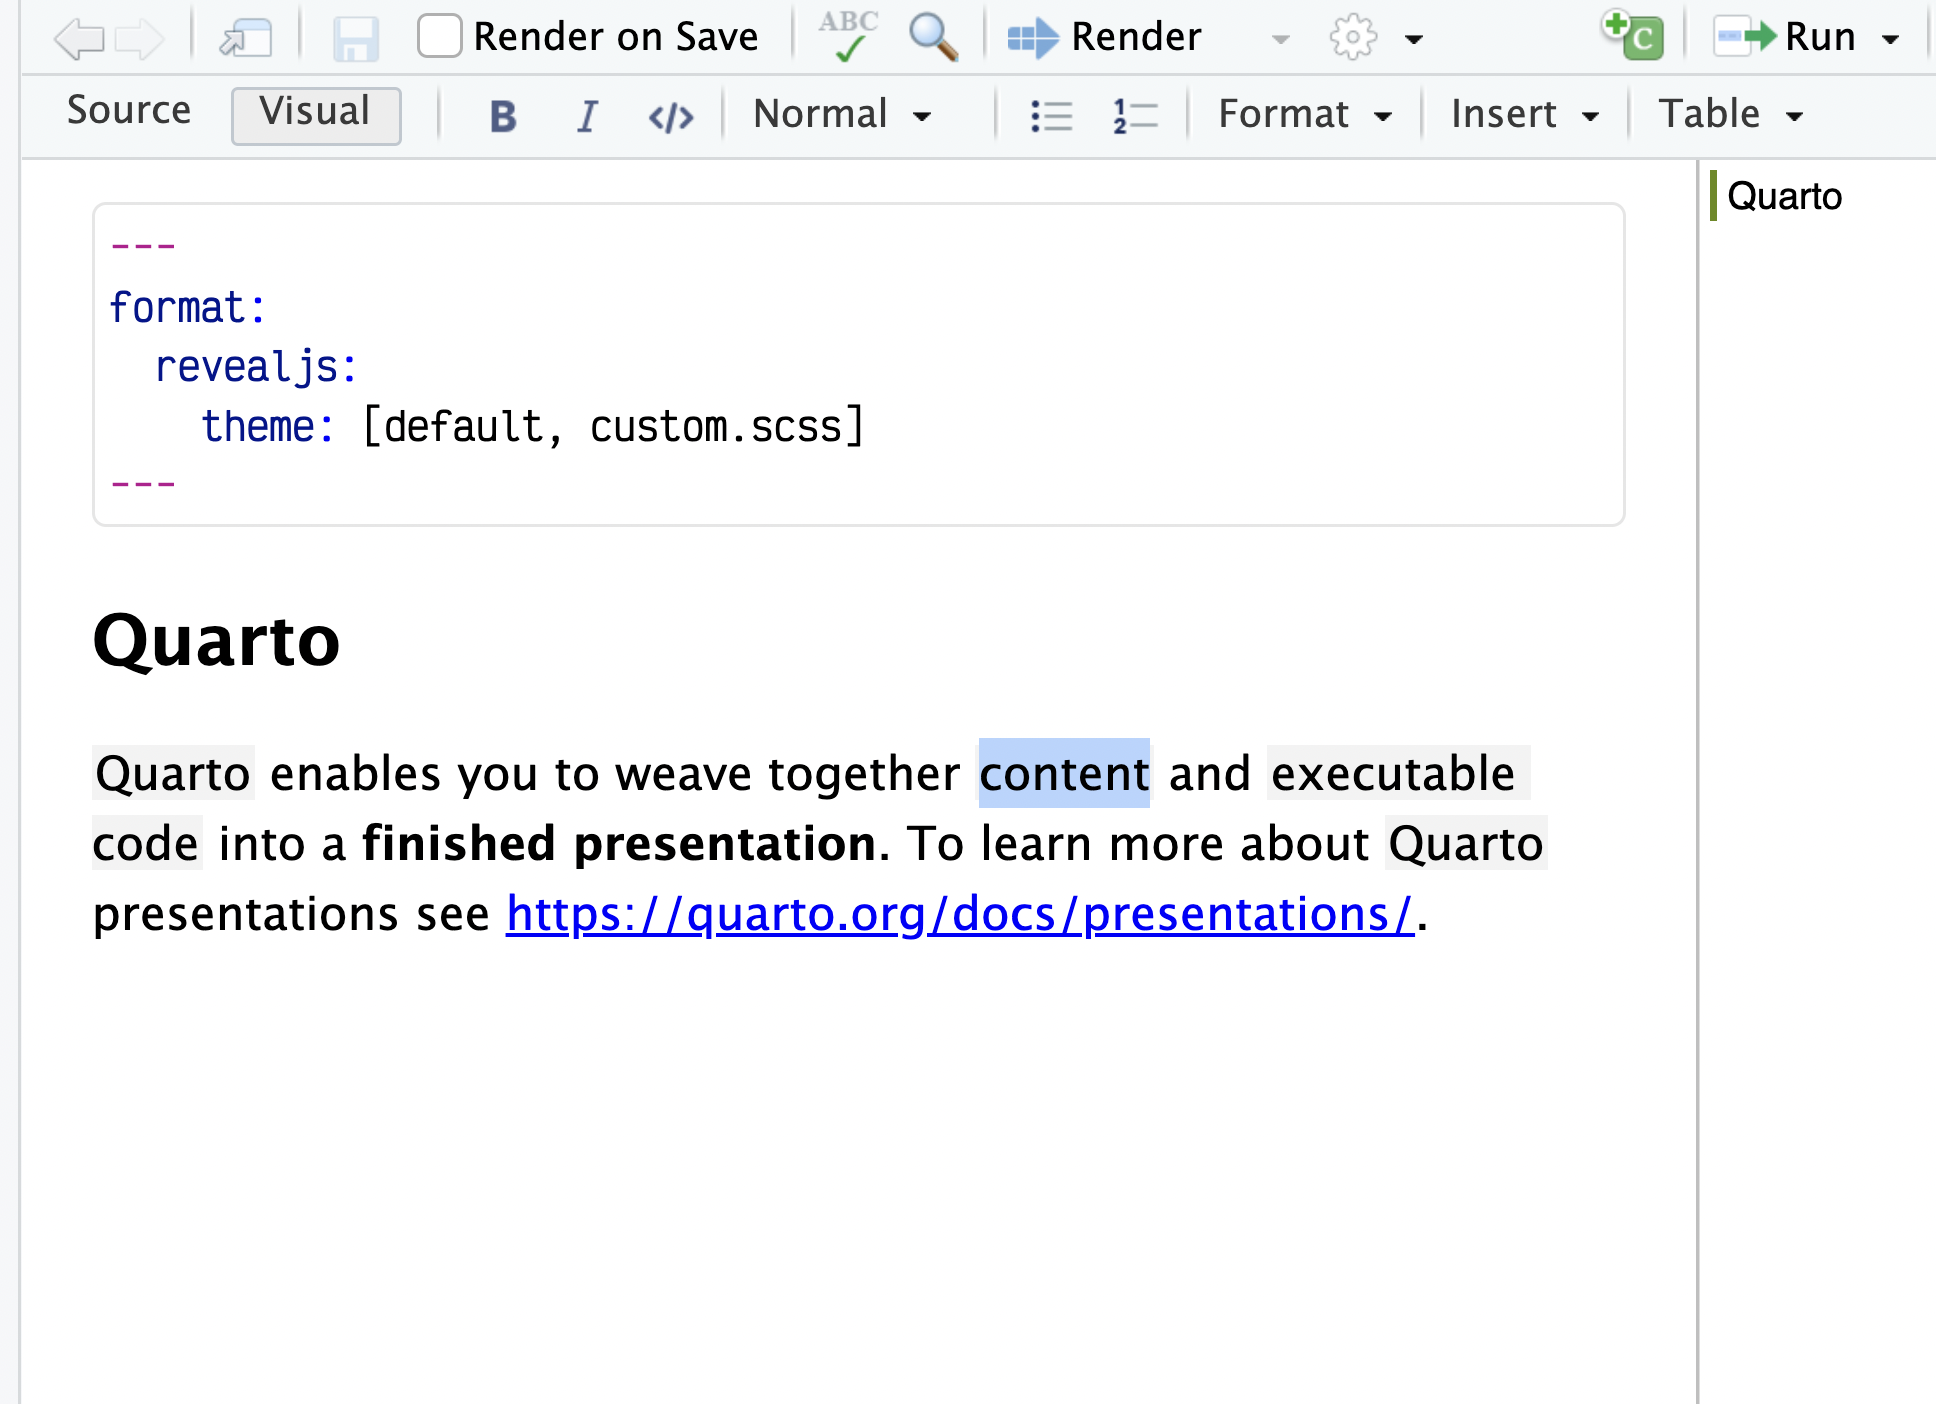
\includegraphics[keepaspectratio]{media/apply-class-1.png}}

Click ``Format'' and select ``Span\ldots{}'' This will only apply the
changes to the highlighted words, instead of the whole paragraph.

\pandocbounded{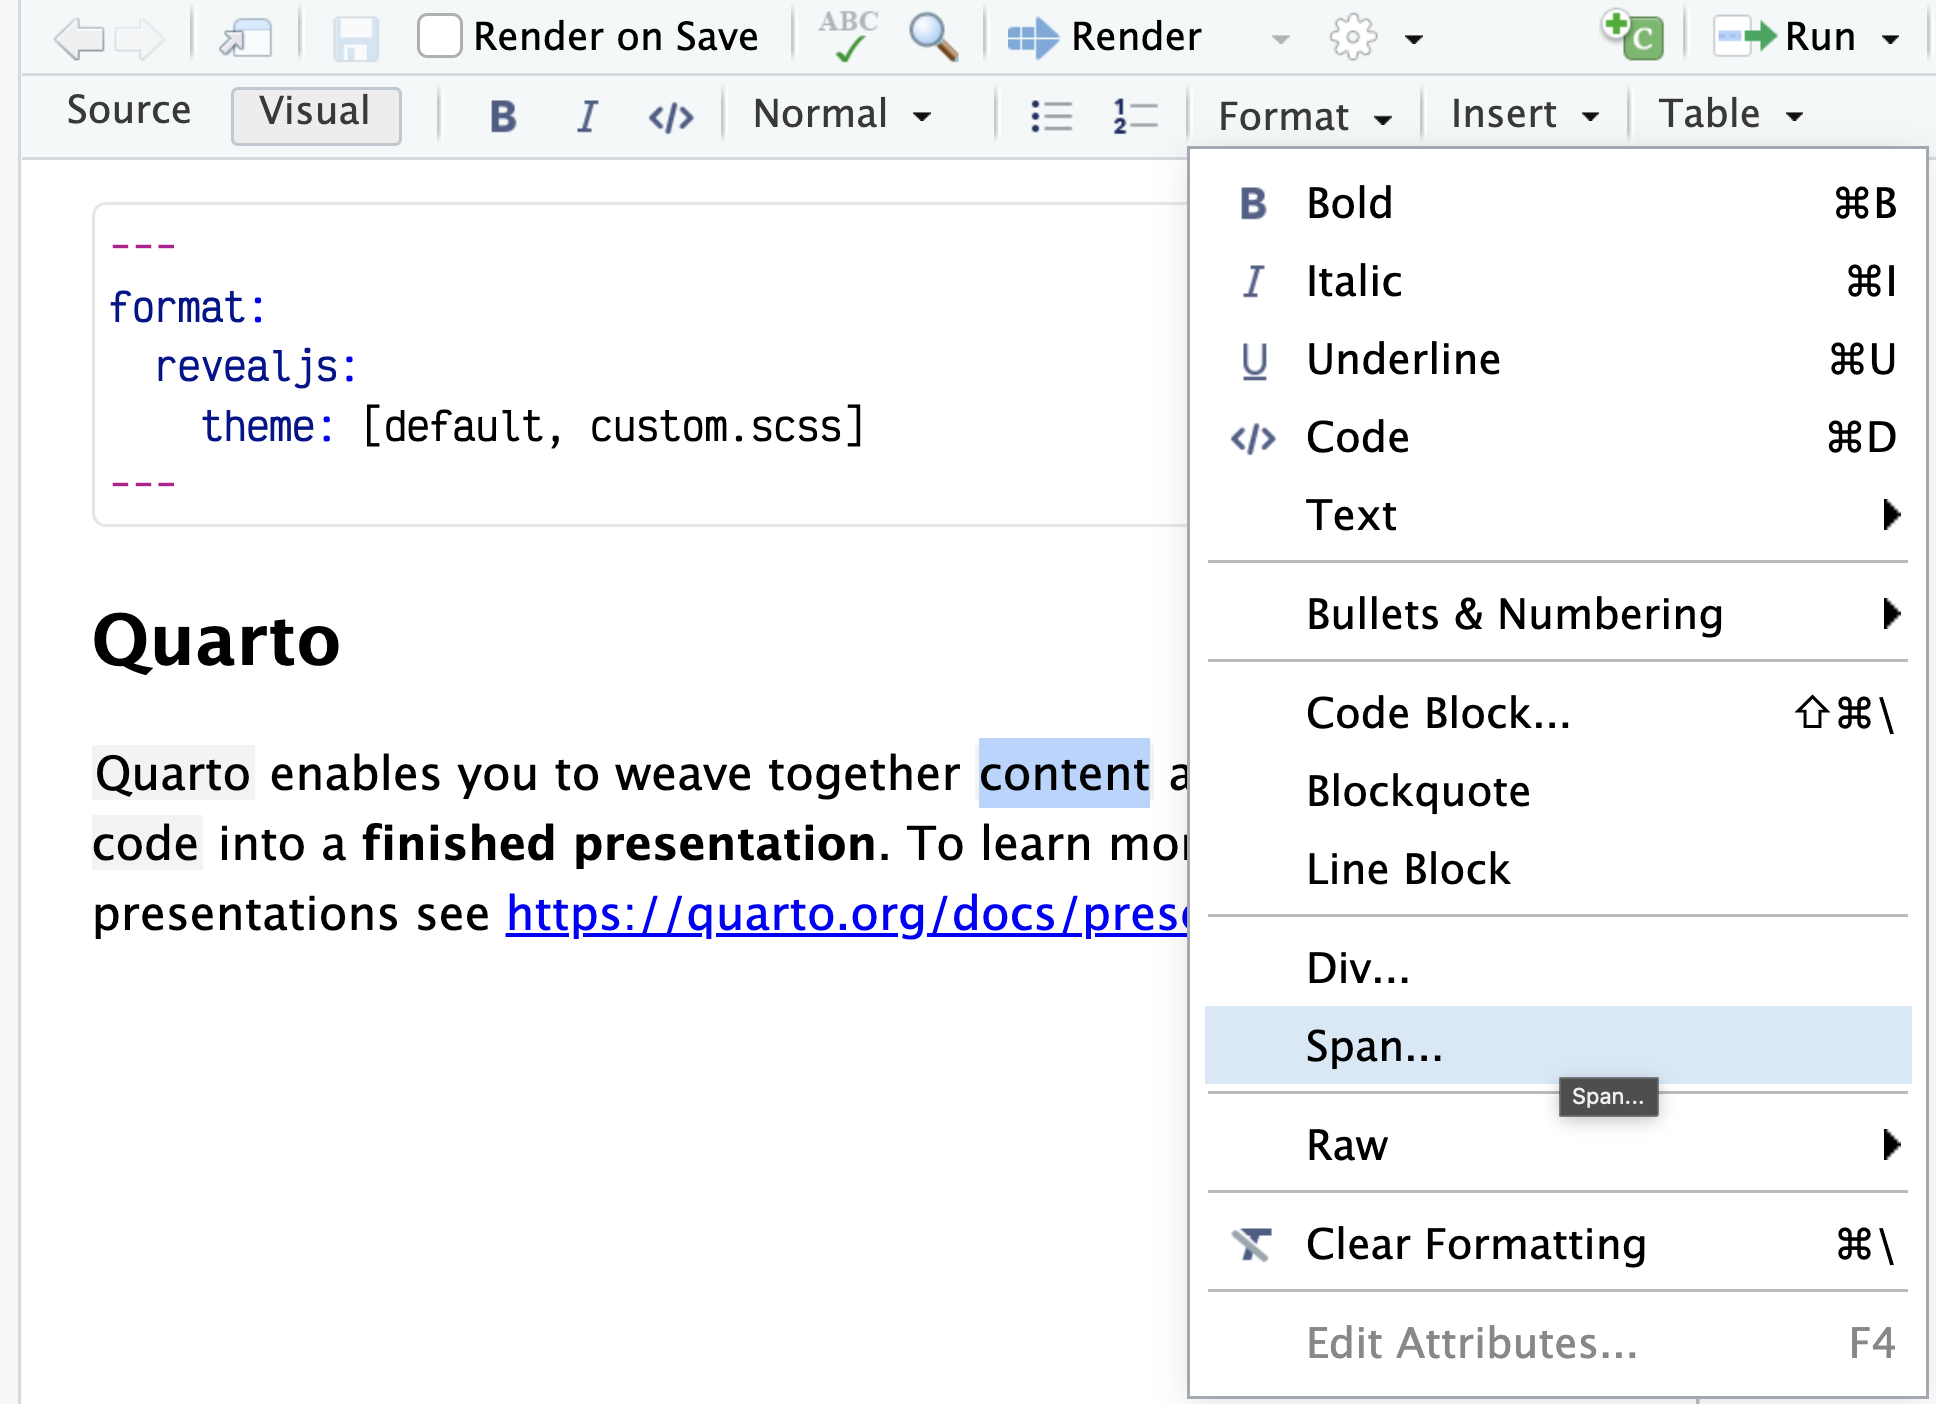
\includegraphics[keepaspectratio]{media/apply-class-2.png}}

And then write in the class name in the ``Classes'' field. We see the
word yellow by using the class ``.yellow''.

\pandocbounded{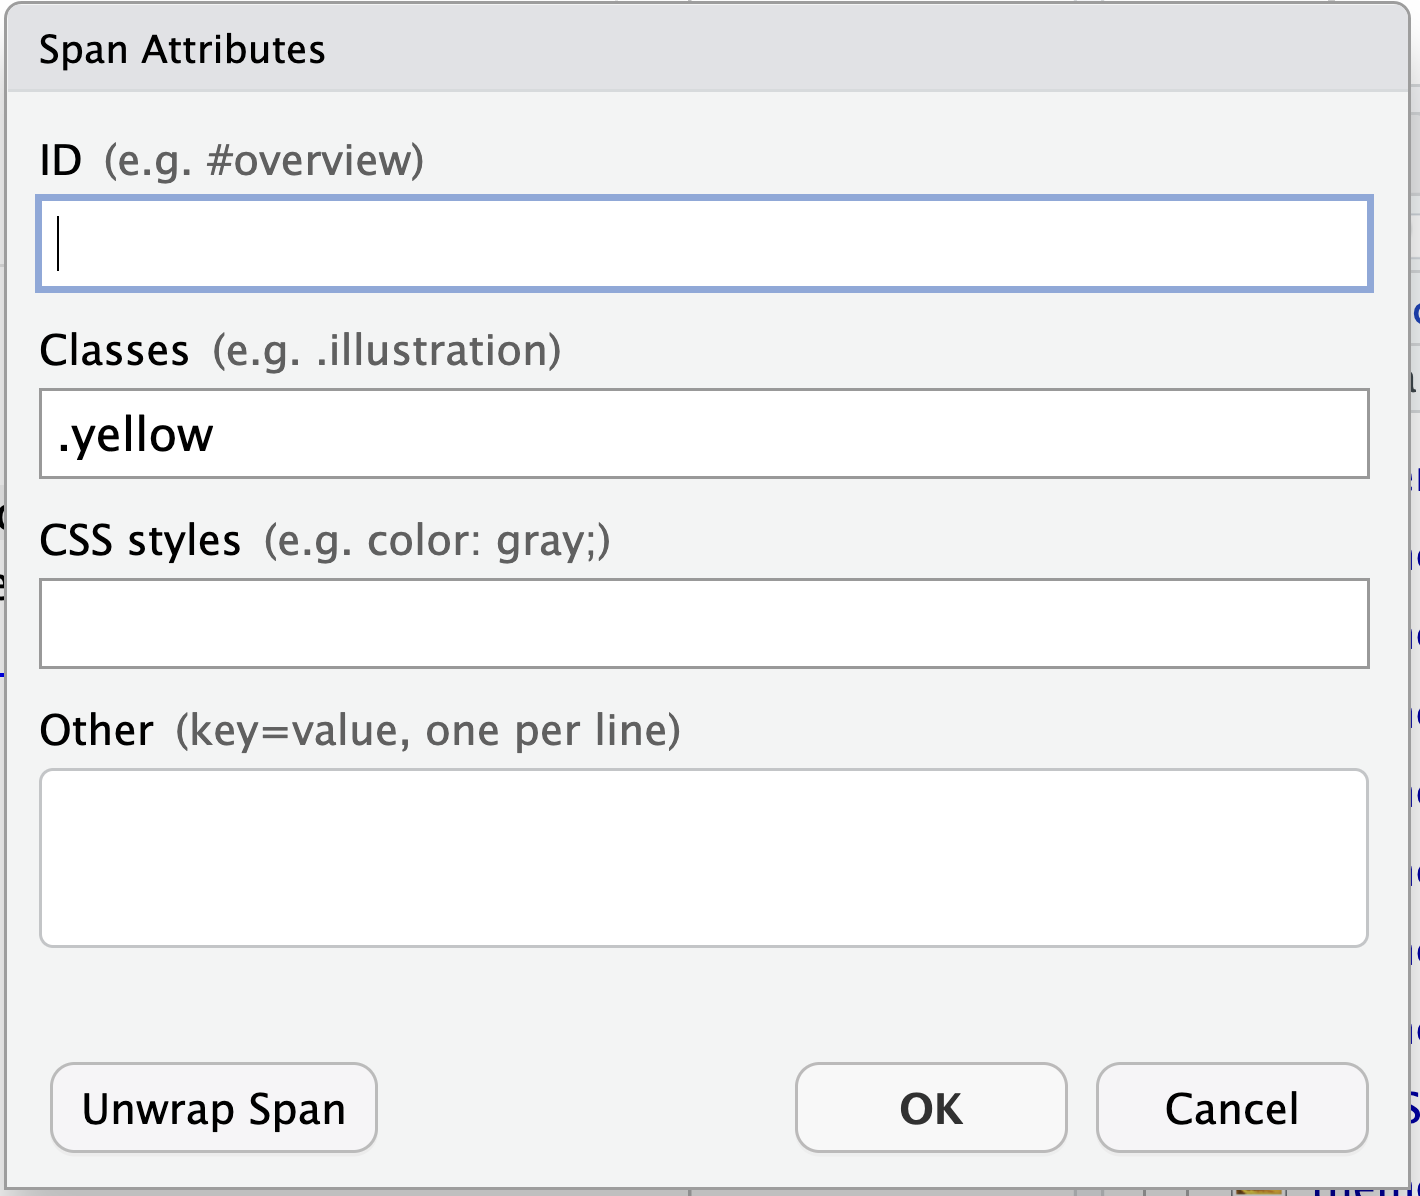
\includegraphics[keepaspectratio]{media/apply-class-3.png}}

We can also apply these changes in the source editor by using the
\texttt{{[}text{]}\{.class\}} syntax. I added (slightly excessive)
highlighting to a couple of words. See below

\begin{Shaded}
\begin{Highlighting}[]
\CommentTok{[}\OtherTok{Quarto}\CommentTok{]}\NormalTok{\{.blue\} enables you to weave together }\CommentTok{[}\OtherTok{content}\CommentTok{]}\NormalTok{\{.yellow\} and }\CommentTok{[}\OtherTok{executable code}\CommentTok{]}\NormalTok{\{.yellow\} into a **finished presentation**. To learn more about }\CommentTok{[}\OtherTok{Quarto}\CommentTok{]}\NormalTok{\{.blue\} presentations see }\OtherTok{\textless{}https://quarto.org/docs/presentations/\textgreater{}}\NormalTok{.}
\end{Highlighting}
\end{Shaded}

And we get the following slide

\pandocbounded{
\includegraphics[keepaspectratio]{media/theme-example-highlight.png}}

CSS classes were a game changer for my slide-making. It is a little bit
more manual, but if you can write the CSS you can apply it to your
slides which IMO is a super powerful tool.

There are also changes where you just want to modify the CSS directly,
these changes should also be applied in the \texttt{scss:rules} section.
For example, in our example so far, we have used the blue color both to
color the links, and as a highlighting color. This is very confusing, so
let us make sure that all links are underlined. We can make this happen
by adding.

Note that CSS rules that target Reveal content generally need to use the
\texttt{.reveal\ .slide} prefix to successfully override the theme's
default styles.

\begin{Shaded}
\begin{Highlighting}[]
\FunctionTok{.reveal} \FunctionTok{.slide}\NormalTok{ a \{}
  \KeywordTok{text{-}decoration}\NormalTok{: }\DecValTok{underline}\OperatorTok{;}
\NormalTok{\}}
\end{Highlighting}
\end{Shaded}

And the changes have been applied.

\pandocbounded{
\includegraphics[keepaspectratio]{media/example-theme-links.png}}

\section{Style Code}\label{style-code}

to start with we need some code that produces some output, I'll use the
following dplyr example, but any code and language will work the same.
Notice how we are setting \texttt{echo:\ true} to include the source
code in the output.

\begin{Shaded}
\begin{Highlighting}[]
\StringTok{\textasciigrave{}\textasciigrave{}\textasciigrave{}}\AttributeTok{r}
\AttributeTok{\#| echo: true}
\AttributeTok{library(dplyr)}

\AttributeTok{starwars \%\textgreater{}\% }
\AttributeTok{  mutate(name, bmi = mass / ((height / 100)  \^{} 2)) \%\textgreater{}\%}
\AttributeTok{  select(name:mass, bmi)}
\StringTok{\textasciigrave{}\textasciigrave{}\textasciigrave{}}
\end{Highlighting}
\end{Shaded}

without any styling, this gives us the following slide

\pandocbounded{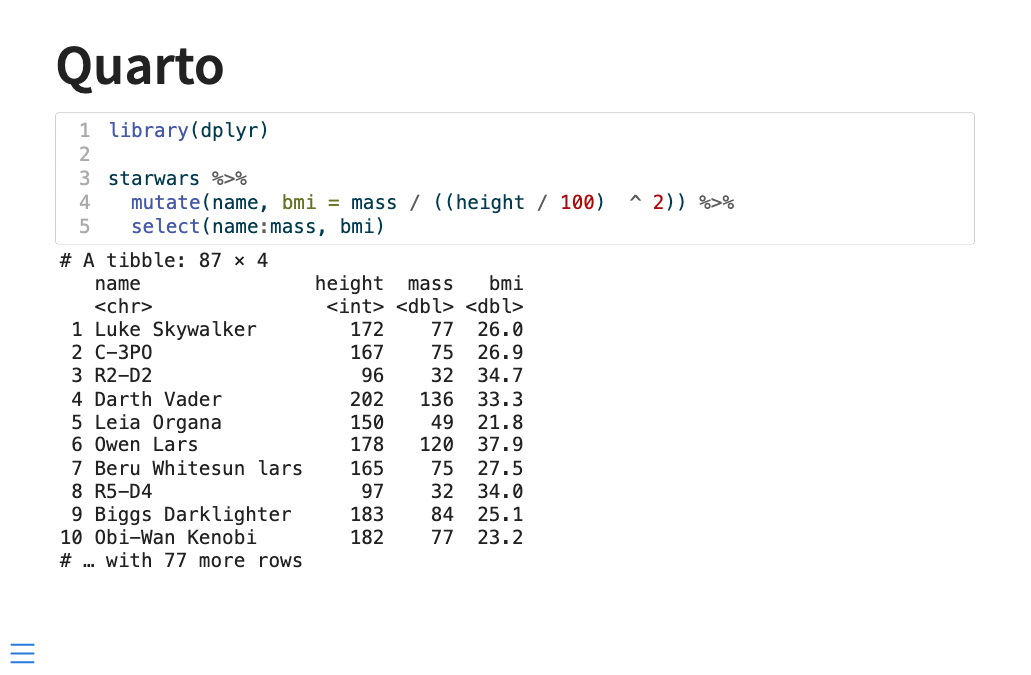
\includegraphics[keepaspectratio]{media/code-no-style.png}}

Now we have a couple of my favorite quarto arguments and then some CSS.

First, we have \texttt{code-copy} and \texttt{code-link} which both can
be found in
\href{https://quarto.org/docs/reference/formats/presentations/revealjs.html\#code}{quarto
revealjs reference}. \texttt{code-copy} adds a little icon that when
clicked copies the entire code block (super useful for
teaching/reference slides) and \texttt{code-link} allows you to have
\href{https://downlit.r-lib.org/}{downlit} add clickable links to
function in the code.

Lastly, I will point out \texttt{code-line-numbers}. This argument can
either turn off or on the line numbers in the code block. This is nice
and has a lot of benefits. Firstly you can turn off the numbering if you
don't find that it is a good use of slide real estate. Secondly, you can
specify line numbers to be put into focus. So setting
\texttt{code-line-numbers:\ "1,3"} in the above example yields us the
following output

\pandocbounded{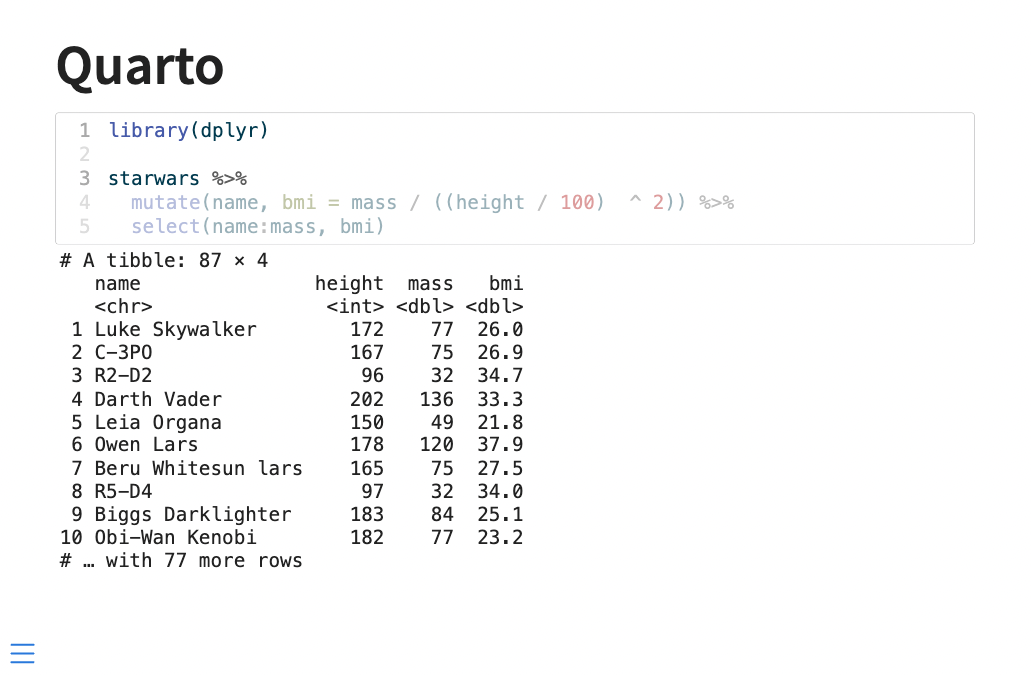
\includegraphics[keepaspectratio]{media/example-code-line-numbers.png}}

Which is a quick and easy way for you to direct the viewer's attention.

Next, let us talk about some styling. Before we do anything custom
ourselves I should note that the 10 different built-in themes also
affect the styling of the code and output, and these might give you what
you need.

If you want to do a little bit more you need to get your hands dirty
with some CSS and SCSS. Much like we did in the
\href{https://www.emilhvitfeldt.com/post/slidecraft-colors-fonts/\#applying-colors}{first
blog post} we are setting up a theme and applying it. I'm going with
this new sandy background color I found.

\pandocbounded{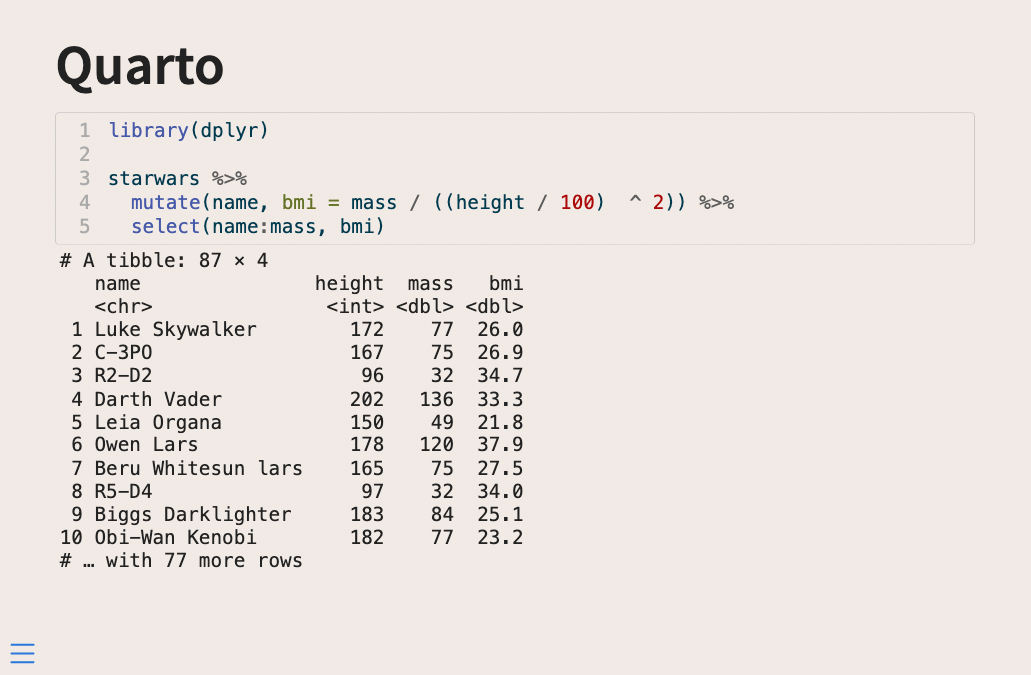
\includegraphics[keepaspectratio]{media/example-sand.png}}

what I don't like about this slide right now is that the code block
doesn't stand out that much. We have 3 major sass variables I want to
introduce today; \texttt{\$code-block-bg},
\texttt{\$code-block-border-color}, and \texttt{\$code-block-font-size}.
\texttt{\$code-block-bg} as the name suggests modifies the background of
the code block, setting this color to white makes the code pop a little
bit more

\pandocbounded{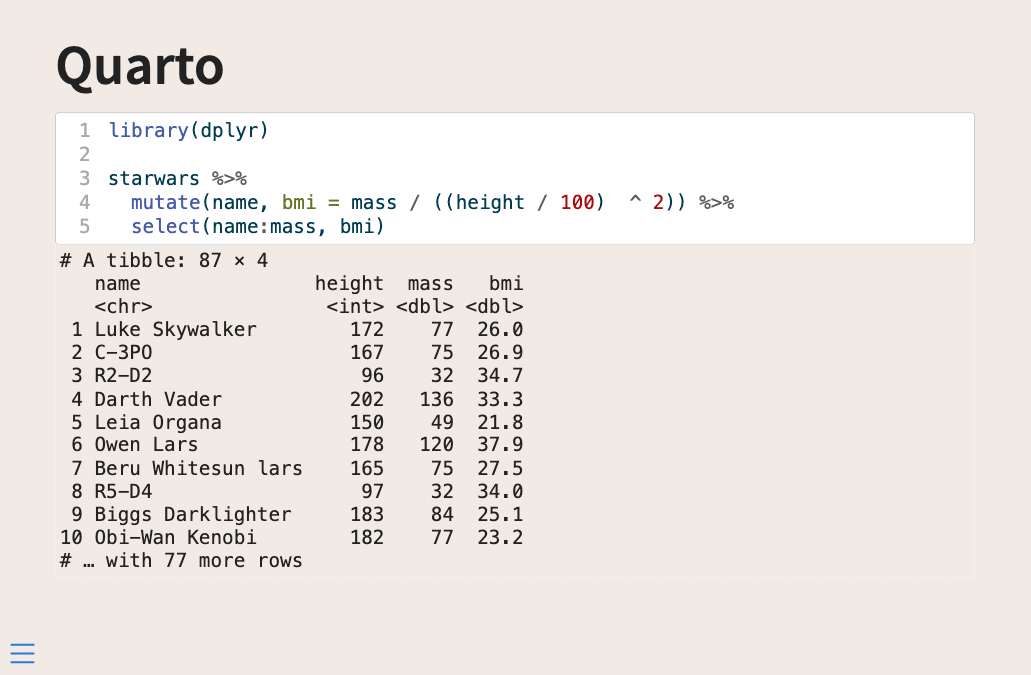
\includegraphics[keepaspectratio]{media/example-sand-white.png}}

We can also change the border color with
\texttt{\$code-block-border-color}. This quantity defaults to being a
lightened version of the main text color. We can instead set it to be a
slightly darker version of the background color by setting
\texttt{\$code-block-border-color:\ darken(\$body-bg,\ 20\%);} and
getting this

\pandocbounded{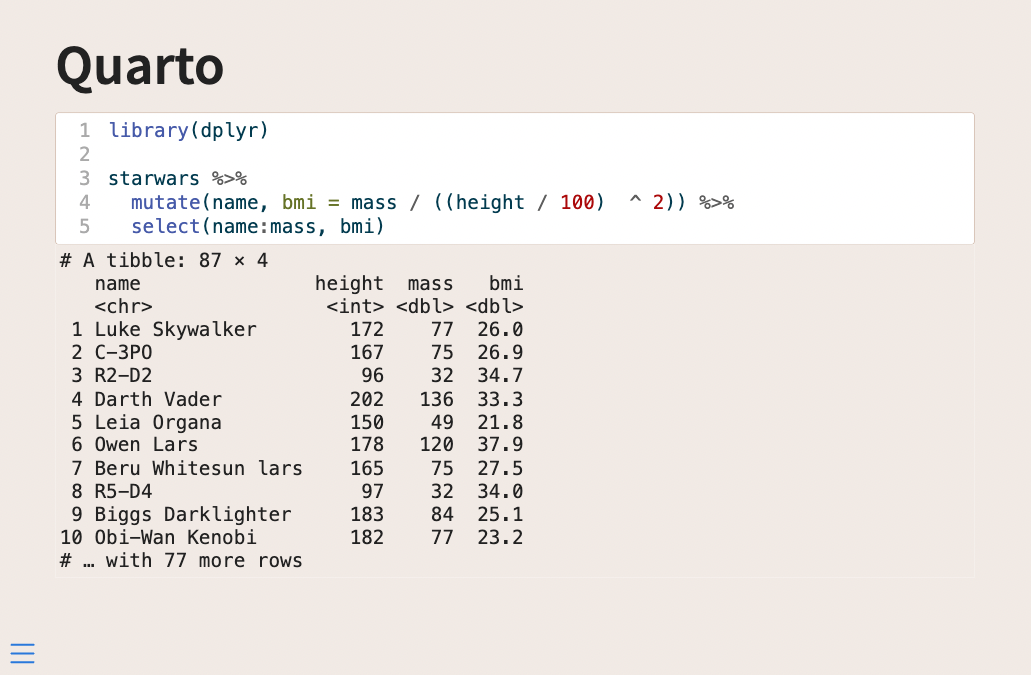
\includegraphics[keepaspectratio]{media/example-sand-border-dark.png}}

Or remove it entirely by setting it to be transparent with
\texttt{\$code-block-border-color:\ \#00000000;}, for this look:

\pandocbounded{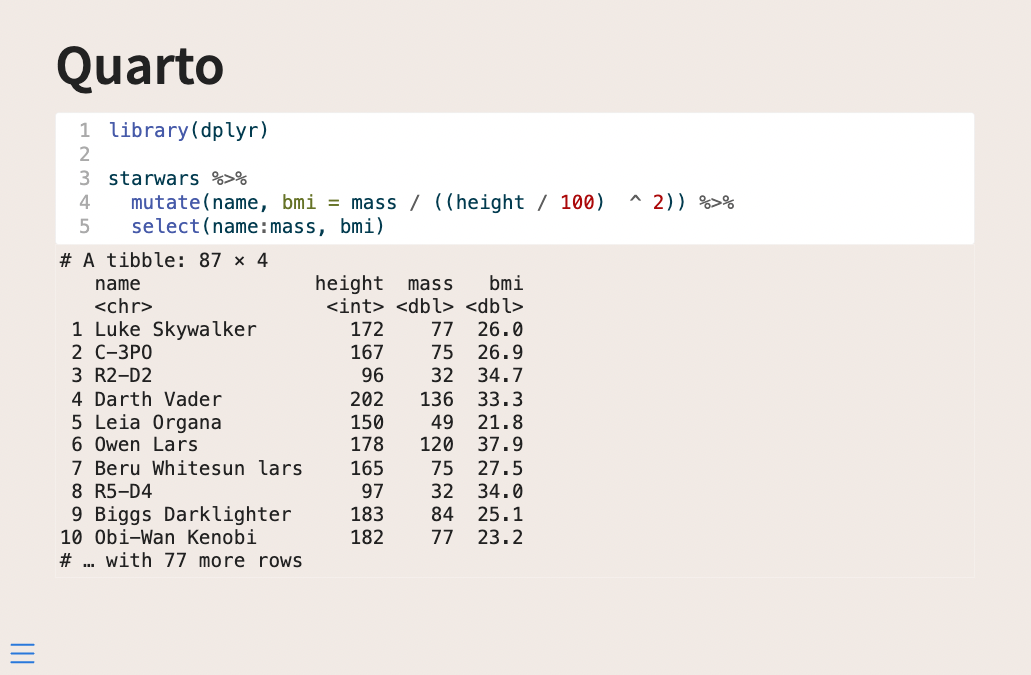
\includegraphics[keepaspectratio]{media/example-sand-no-border.png}}

Lastly, we can change the font size with
\texttt{\$code-block-font-size}. While the size is pretty good right
now, it is important that we know how to change it as it will depend on
the fonts we use throughout the theme.

Below is an example where I turned up the size every so slightly

\pandocbounded{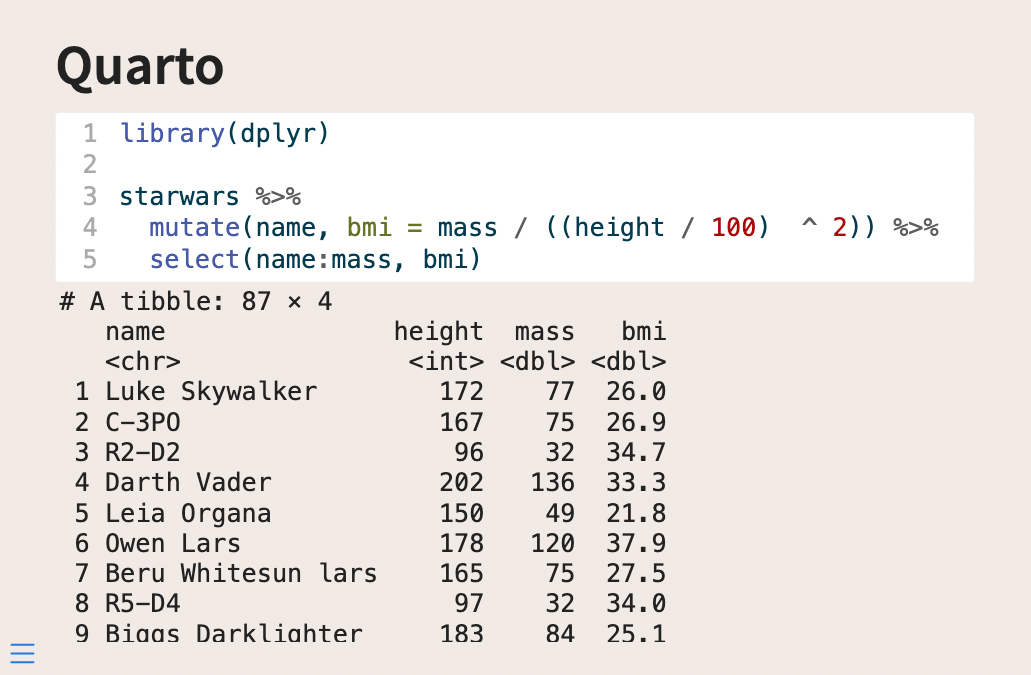
\includegraphics[keepaspectratio]{media/sand-large-text.png}}

\section{Style Output}\label{style-output}

The next thing we want to look at is how to style the output. I found
that adding styles to \texttt{.reveal\ pre\ code} did the trick in only
changing the output, not the source.

Using the following code in our \texttt{.scss} file

\begin{Shaded}
\begin{Highlighting}[]
\CommentTok{/*{-}{-} scss:rules {-}{-}*/}

\FunctionTok{.reveal}\NormalTok{ pre code \{}
  \KeywordTok{background{-}color}\NormalTok{: }\ConstantTok{\#FFFFFF}\OperatorTok{;}
\NormalTok{\}}
\end{Highlighting}
\end{Shaded}

Will give us the following output

\pandocbounded{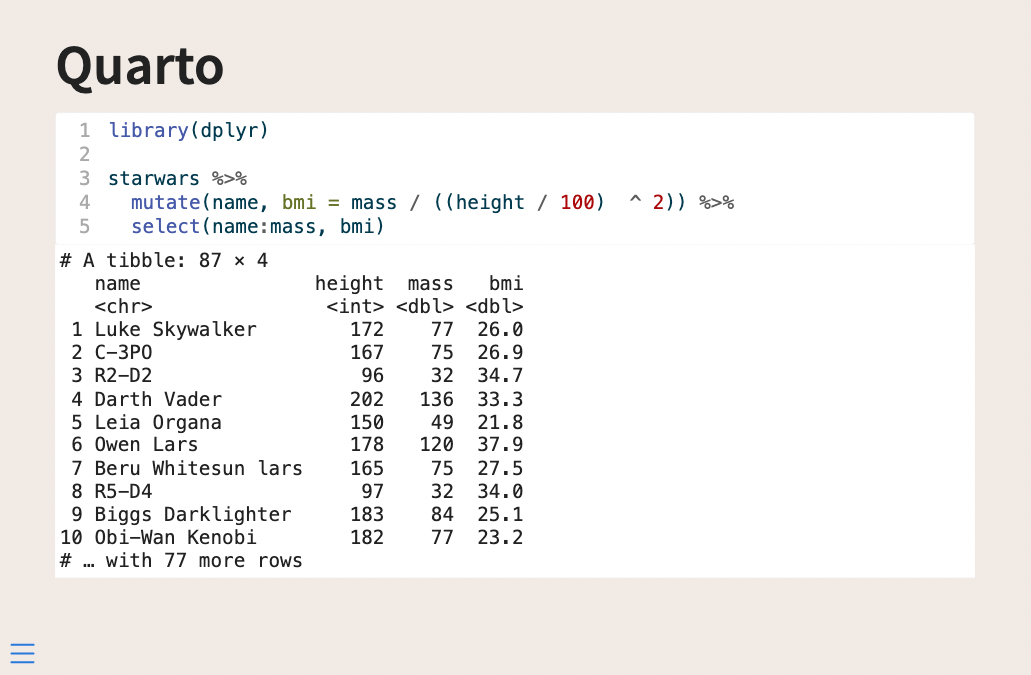
\includegraphics[keepaspectratio]{media/example-output-white.png}}

Which is already Quite a bit better. For this, I would do either one of
two things.

\begin{itemize}
\tightlist
\item
  Make the source and output appear to be one large box
\item
  Separate the source and output more clearly
\end{itemize}

Let us see how we can do both of these things.

To make the source and output appear as one, we need to modify the
source box, since it has a little bit of a border that is making them
unequal. Setting \texttt{.reveal\ div.sourceCode\ \{border:\ none\}}
should remove the existing border, and we can remove the slight rounded
border as well by also adding \texttt{border-radius:\ 0px;}. This gives
a full \texttt{.scss} as follows

\begin{Shaded}
\begin{Highlighting}[]
\CommentTok{/*{-}{-} scss:defaults {-}{-}*/}
\VariableTok{$theme{-}sand}\NormalTok{: }\ConstantTok{\#F1EAE5}\OperatorTok{;}
\VariableTok{$theme{-}white}\NormalTok{: }\ConstantTok{\#FFFFFF}\OperatorTok{;}

\VariableTok{$body{-}bg}\NormalTok{: }\VariableTok{$theme{-}sand}\OperatorTok{;}
\VariableTok{$code{-}block{-}bg}\NormalTok{: }\VariableTok{$theme{-}white}\OperatorTok{;}

\CommentTok{/*{-}{-} scss:rules {-}{-}*/}
\FunctionTok{.reveal}\NormalTok{ pre code \{}
  \KeywordTok{background{-}color}\NormalTok{: }\VariableTok{$theme{-}white}\OperatorTok{;}
\NormalTok{\}}

\FunctionTok{.reveal}\NormalTok{ div}\FunctionTok{.sourceCode}\NormalTok{ \{}
  \KeywordTok{border}\NormalTok{: }\DecValTok{none}\OperatorTok{;}
  \KeywordTok{border{-}radius}\NormalTok{: }\DecValTok{0}\DataTypeTok{px}\OperatorTok{;}
\NormalTok{\}}
\end{Highlighting}
\end{Shaded}

This gives us the following slides

\pandocbounded{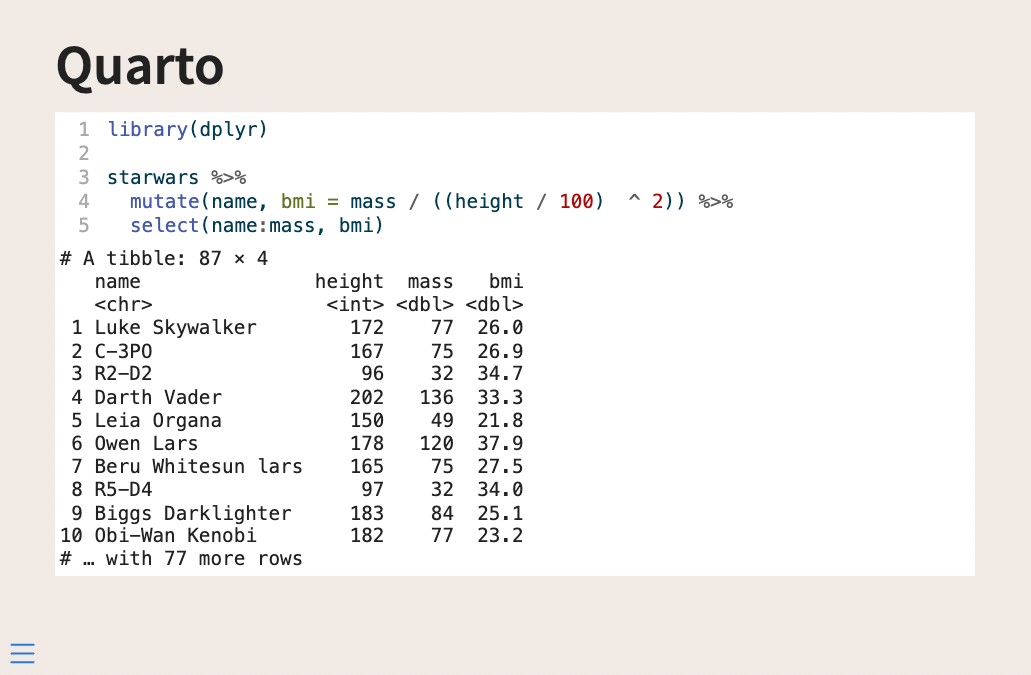
\includegraphics[keepaspectratio]{media/example-white-no-border.png}}

If we want some space, we can add
\texttt{margin-bottom:\ 10px\ !important;} to the
\texttt{.reveal\ div.sourceCode} specification, making it so there will
be 10 pixels worth of space below the source, which gives some spacing
between the two boxes. You need the \texttt{!important} to overwrite a
more general style specification.

Making it so that part of the \texttt{.scss} file now looks like this

\begin{Shaded}
\begin{Highlighting}[]
\FunctionTok{.reveal}\NormalTok{ div}\FunctionTok{.sourceCode}\NormalTok{ \{}
  \KeywordTok{border}\NormalTok{: }\DecValTok{none}\OperatorTok{;}
  \KeywordTok{border{-}radius}\NormalTok{: }\DecValTok{0}\DataTypeTok{px}\OperatorTok{;}
  \KeywordTok{margin{-}bottom}\NormalTok{: }\DecValTok{10}\DataTypeTok{px} \AttributeTok{!important}\OperatorTok{;}
\NormalTok{\}}
\end{Highlighting}
\end{Shaded}

And you now have a little bit of air between the boxes

\pandocbounded{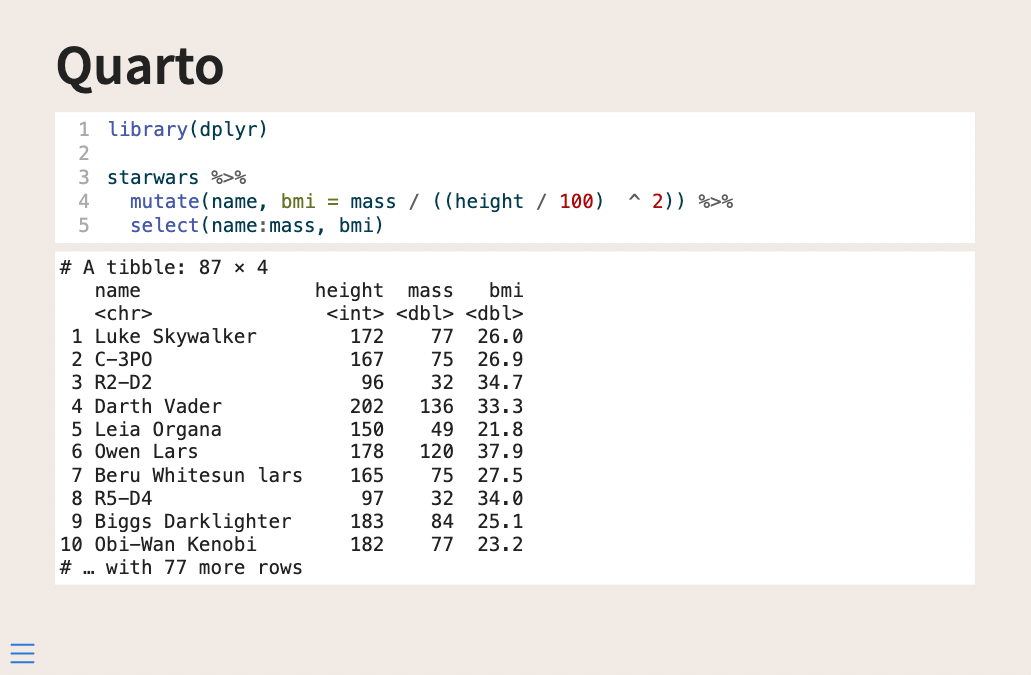
\includegraphics[keepaspectratio]{media/example-little-bit-of-air.png}}

\section{Change highlighting theme}\label{change-highlighting-theme}

One thing we haven't looked at yet is how to change the highlighting
theme. We will see how we can do that here. This is an often overlooked
part of a presentation, that if you spend some time can tie your
presentation together.

This is being controlled in the \texttt{highlight-style} argument. I
would generally recommend that you set this option globally in your
document by including it in your YAML file like so

\begin{Shaded}
\begin{Highlighting}[]
\PreprocessorTok{{-}{-}{-}}
\FunctionTok{format}\KeywordTok{:}
\AttributeTok{  }\FunctionTok{revealjs}\KeywordTok{:}\AttributeTok{ }
\AttributeTok{    }\FunctionTok{theme}\KeywordTok{:}\AttributeTok{ }\KeywordTok{[}\AttributeTok{default}\KeywordTok{,}\AttributeTok{ custom.scss}\KeywordTok{]}
\FunctionTok{highlight{-}style}\KeywordTok{:}\AttributeTok{ }\StringTok{"dracula"}
\PreprocessorTok{{-}{-}{-}}
\end{Highlighting}
\end{Shaded}

Which would result in the following output

\pandocbounded{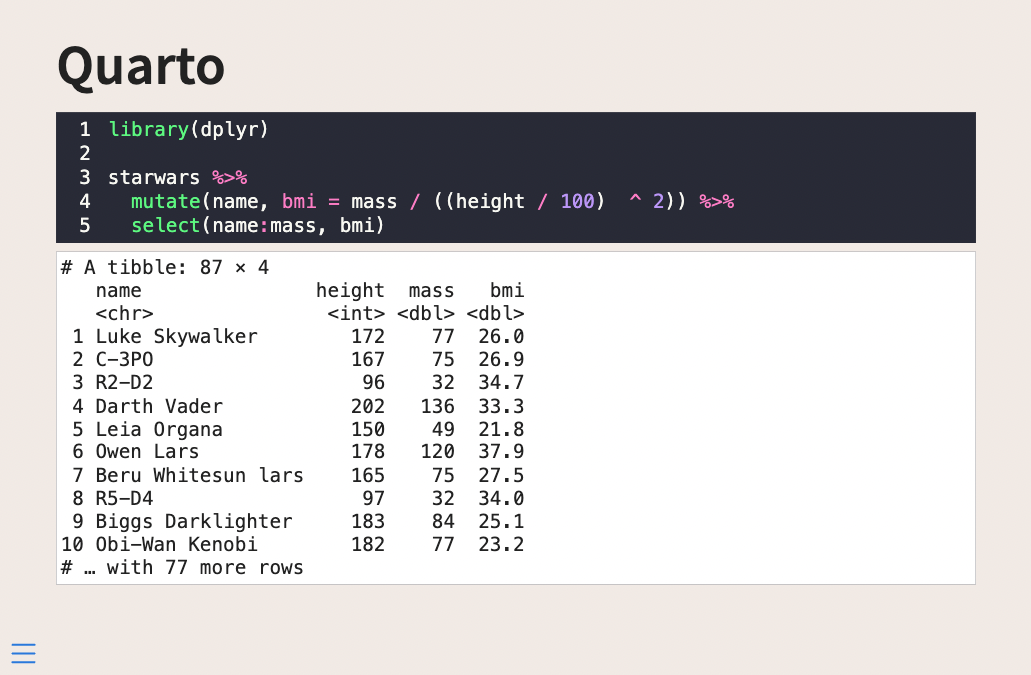
\includegraphics[keepaspectratio]{media/example-dracula.png}}

\begin{tcolorbox}[enhanced jigsaw, titlerule=0mm, bottomrule=.15mm, opacityback=0, colbacktitle=quarto-callout-warning-color!10!white, colframe=quarto-callout-warning-color-frame, coltitle=black, breakable, toprule=.15mm, colback=white, bottomtitle=1mm, title=\textcolor{quarto-callout-warning-color}{\faExclamationTriangle}\hspace{0.5em}{Warning}, toptitle=1mm, arc=.35mm, left=2mm, leftrule=.75mm, rightrule=.15mm, opacitybacktitle=0.6]

Some of the themes such as the \texttt{"dracula"} theme come with a
built-in background color. If you set \texttt{\$code-block-bg} in your
\texttt{.scss} file it will be overwritten.

\end{tcolorbox}

\begin{Shaded}
\begin{Highlighting}[]
\FunctionTok{\{}
    \DataTypeTok{"text{-}color"}\FunctionTok{:} \KeywordTok{null}\FunctionTok{,}
    \DataTypeTok{"background{-}color"}\FunctionTok{:} \StringTok{"\#f8f8f8"}\FunctionTok{,}
    \DataTypeTok{"line{-}number{-}color"}\FunctionTok{:} \StringTok{"\#aaaaaa"}\FunctionTok{,}
    \DataTypeTok{"line{-}number{-}background{-}color"}\FunctionTok{:} \KeywordTok{null}\FunctionTok{,}
    \DataTypeTok{"text{-}styles"}\FunctionTok{:} \FunctionTok{\{}
        \DataTypeTok{"Other"}\FunctionTok{:} \FunctionTok{\{}
            \DataTypeTok{"text{-}color"}\FunctionTok{:} \StringTok{"\#8f5902"}\FunctionTok{,}
            \DataTypeTok{"background{-}color"}\FunctionTok{:} \KeywordTok{null}\FunctionTok{,}
            \DataTypeTok{"bold"}\FunctionTok{:} \KeywordTok{false}\FunctionTok{,}
            \DataTypeTok{"italic"}\FunctionTok{:} \KeywordTok{false}\FunctionTok{,}
            \DataTypeTok{"underline"}\FunctionTok{:} \KeywordTok{false}
        \FunctionTok{\},}
        \DataTypeTok{"Attribute"}\FunctionTok{:} \FunctionTok{\{}
            \DataTypeTok{"text{-}color"}\FunctionTok{:} \StringTok{"\#c4a000"}\FunctionTok{,}
            \DataTypeTok{"background{-}color"}\FunctionTok{:} \KeywordTok{null}\FunctionTok{,}
            \DataTypeTok{"bold"}\FunctionTok{:} \KeywordTok{false}\FunctionTok{,}
            \DataTypeTok{"italic"}\FunctionTok{:} \KeywordTok{false}\FunctionTok{,}
            \DataTypeTok{"underline"}\FunctionTok{:} \KeywordTok{false}
        \FunctionTok{\},}
\end{Highlighting}
\end{Shaded}

There are
\href{https://github.com/quarto-dev/quarto-cli/tree/main/src/resources/pandoc/highlight-styles}{many
different highlighting themes} that come shipped with Quarto. The ones
with \texttt{-dark} and \texttt{-light} postfixes are themes that will
adjust depending on whether your slides are dark or light.

If none of these are what you want, you can create your own. I would
suggest taking one of the themes you like from the list linked above and
modifying it to your liking. Copy that file into the same directory as
your slides, and point to the file name instead. Like so:

\begin{Shaded}
\begin{Highlighting}[]
\PreprocessorTok{{-}{-}{-}}
\FunctionTok{format}\KeywordTok{:}
\AttributeTok{  }\FunctionTok{revealjs}\KeywordTok{:}\AttributeTok{ }
\AttributeTok{    }\FunctionTok{theme}\KeywordTok{:}\AttributeTok{ }\KeywordTok{[}\AttributeTok{default}\KeywordTok{,}\AttributeTok{ custom.scss}\KeywordTok{]}
\FunctionTok{highlight{-}style}\KeywordTok{:}\AttributeTok{ }\StringTok{"darkula.theme"}
\PreprocessorTok{{-}{-}{-}}
\end{Highlighting}
\end{Shaded}

If your slides use both dark and light backgrounds you will likely need
two sets of highlighting theme files, which you can set with:

\begin{Shaded}
\begin{Highlighting}[]
\PreprocessorTok{{-}{-}{-}}
\FunctionTok{format}\KeywordTok{:}
\AttributeTok{  }\FunctionTok{revealjs}\KeywordTok{:}\AttributeTok{ }
\AttributeTok{    }\FunctionTok{theme}\KeywordTok{:}\AttributeTok{ }\KeywordTok{[}\AttributeTok{default}\KeywordTok{,}\AttributeTok{ custom.scss}\KeywordTok{]}
\FunctionTok{highlight{-}style}\KeywordTok{:}
\AttributeTok{  }\FunctionTok{light}\KeywordTok{:}\AttributeTok{ light.theme}
\AttributeTok{  }\FunctionTok{dark}\KeywordTok{:}\AttributeTok{ dark.theme}
\PreprocessorTok{{-}{-}{-}}
\end{Highlighting}
\end{Shaded}

I slowly modified the base theme, using the
\href{https://docs.kde.org/trunk5/en/kate/katepart/color-themes.html}{Working
with Color Themes documentation} to help me figure out what the
different names mean.

Another thing that can aid, is opening the developer tools in your
browser and hovering over the kind of elements you care about. Below I
am doing just that, and I see that the pipe is of class \texttt{sc}

\pandocbounded{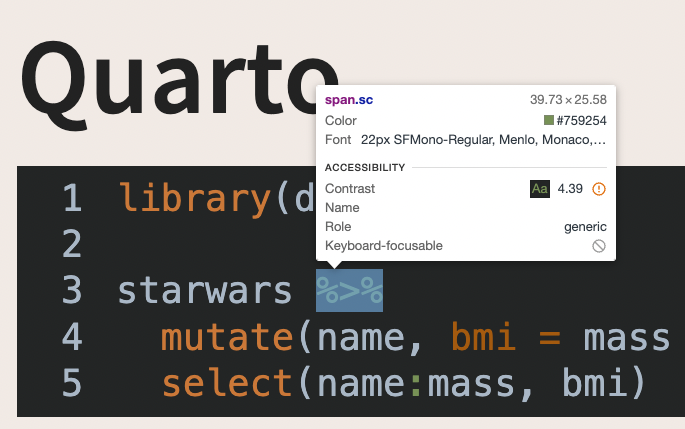
\includegraphics[keepaspectratio]{media/developer-tools.png}}

From that, you can look at this list and see that it is a
\texttt{SpecialChar} and you can modify your theme accordingly.

\begin{itemize}
\tightlist
\item
  ot: \textbf{Other}
\item
  at: \textbf{Attribute}
\item
  ss: \textbf{SpecialString}
\item
  an: \textbf{Annotation}
\item
  fu: \textbf{Function}
\item
  st: \textbf{String}
\item
  cf: \textbf{ControlFlow}
\item
  op: \textbf{Operator}
\item
  er: \textbf{Error}
\item
  bn: \textbf{BaseN}
\item
  al: \textbf{Alert}
\item
  va: \textbf{Variable}
\item
  pp: \textbf{Preprocessor}
\item
  in: \textbf{Information}
\item
  vs: \textbf{VerbatimString}
\item
  wa: \textbf{Warning}
\item
  do: \textbf{Documentation}
\item
  ch: \textbf{Char}
\item
  dt: \textbf{DataType}
\item
  fl: \textbf{Float}
\item
  co: \textbf{Comment}
\item
  cv: \textbf{CommentVar}
\item
  cn: \textbf{Constant}
\item
  sc: \textbf{SpecialChar}
\item
  dv: \textbf{DecVal}
\item
  kw: \textbf{Keyword}
\end{itemize}

With these changes in place, I get to the following slides

\pandocbounded{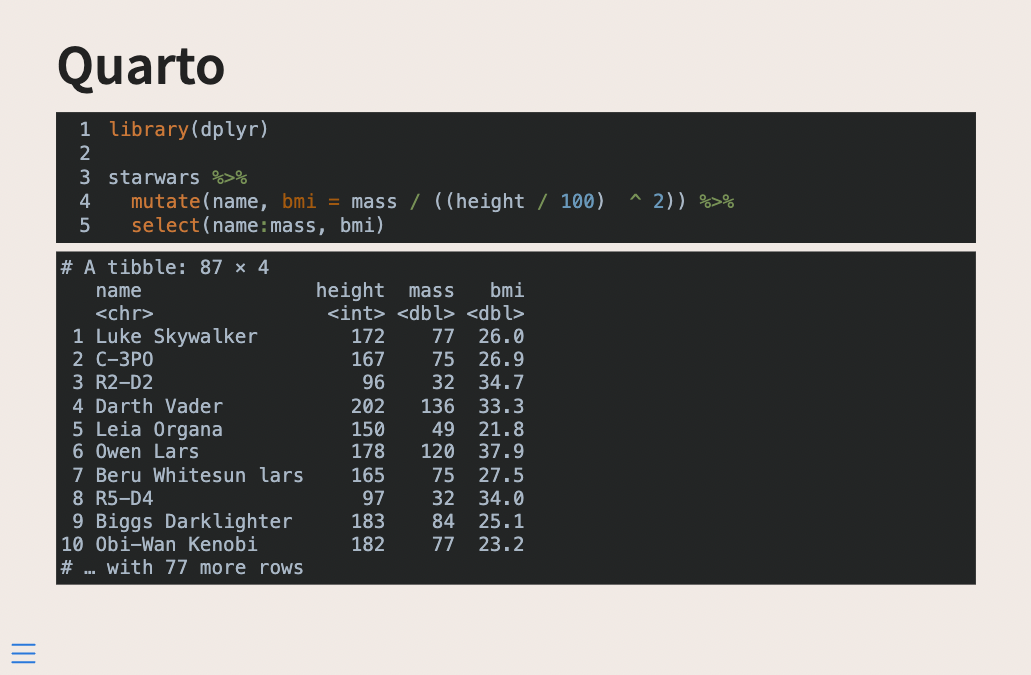
\includegraphics[keepaspectratio]{media/example-darkula.png}}

For this theme, I also updated \texttt{.reveal\ pre\ code} to change the
background color and the text color of the output to match the rest of
the theme.

You generally don't need to update all the items in the theme as you are
unlikely to use all of them. I tend to update as I go, only updating the
classes that I use.

\section{Use fonts with ligatures}\label{use-fonts-with-ligatures}

I just added some new code to a slide

\pandocbounded{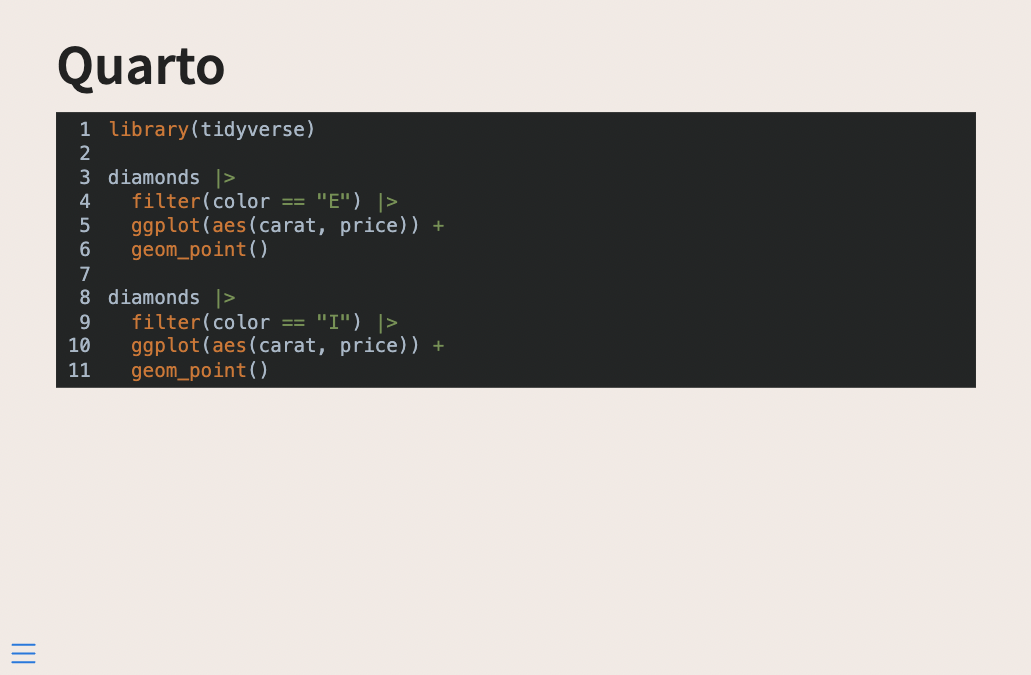
\includegraphics[keepaspectratio]{media/no-ligatures.png}}

and this code uses some multi-character symbols like \texttt{!=} and
\texttt{\textbar{}\textgreater{}}. These and many like them are common
all over the different programming languages, so much so that people
have created special fonts with ligatures to make them prettier.

One such font is \href{https://github.com/tonsky/FiraCode}{FiraCode}.

\pandocbounded{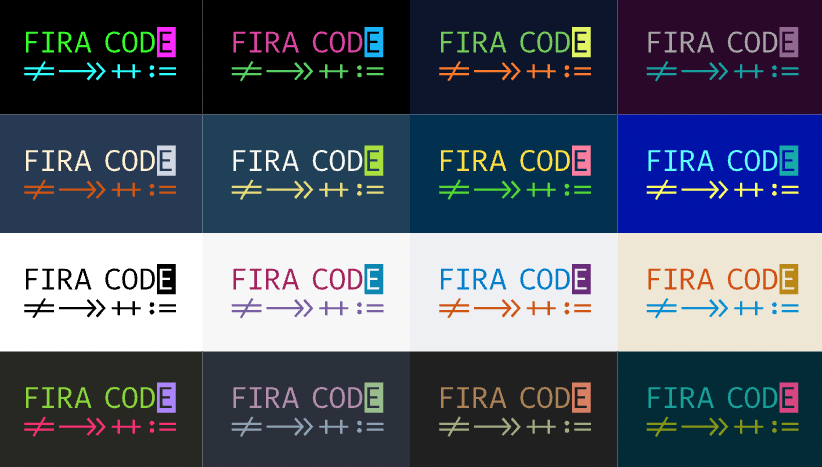
\includegraphics[keepaspectratio]{media/firacode.png}}

And we can add these types of fonts to our slides as well! Start by
downloading the font from the site, and copy over a \texttt{.woff} and
\texttt{.woff2} file to your slide directory. I selected
\texttt{FiraCode-Regular.woff} and \texttt{FiraCode-Regular.woff2}.

In the \texttt{/*-\/-\ scss:defaults\ -\/-*/} part of our \texttt{.scss}
file, we are going to add the following code. This is done to register
the font family from the files we have included and to have it selected
for use for monospace fonts.

\begin{Shaded}
\begin{Highlighting}[]
\ImportTok{@font{-}face}\NormalTok{ \{}
\NormalTok{    font{-}family: }\StringTok{\textquotesingle{}FiraCode\textquotesingle{}}\OperatorTok{;}
\NormalTok{    src: }\FunctionTok{url(}\StringTok{\textquotesingle{}../../../../../FiraCode{-}Regular.woff2\textquotesingle{}}\FunctionTok{)} \FunctionTok{format(}\StringTok{\textquotesingle{}woff2\textquotesingle{}}\FunctionTok{)}\OperatorTok{,}
         \FunctionTok{url(}\StringTok{\textquotesingle{}../../../../../FiraCode{-}Regular.woff\textquotesingle{}}\FunctionTok{)} \FunctionTok{format(}\StringTok{\textquotesingle{}woff\textquotesingle{}}\FunctionTok{)}\OperatorTok{;}
\NormalTok{\}}

\VariableTok{$font{-}family{-}monospace}\NormalTok{: }\StringTok{\textquotesingle{}FiraCode\textquotesingle{}}\OperatorTok{;}
\end{Highlighting}
\end{Shaded}

You might have noticed some ugliness with the \texttt{../../../../../}s.
To my knowledge, this is the best way of using a local font-face from a
file.

With all of that, we now have beautiful ligatures

\pandocbounded{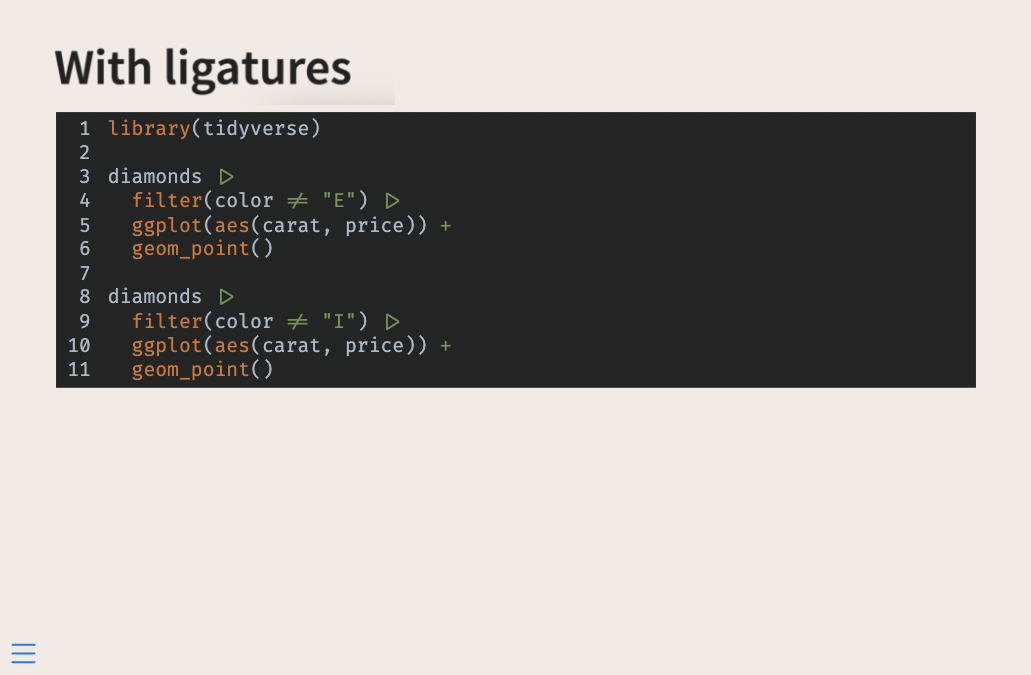
\includegraphics[keepaspectratio]{media/with-ligatures.png}}

\section{Step up your style}\label{step-up-your-style}

Every time I have shared some code with
\href{https://carbon.now.sh/}{carbon.now.sh} people go crazy because it
always looks so good. And I agree, the defaults are really really nice.

So we are going to replicate this. This is going to be a little more
involved, but if you don't have that much code on your slides it will be
a nice touch!

What I do in this case is use
\href{https://reprex.tidyverse.org/}{reprex} to generate the code and
output as one, I paste that into my chunk and turn off evaluation with
\texttt{\#\textbar{}\ eval:\ false}. I do this because then I don't have
to worry about styling the output to match.

I switch over to using the \texttt{"nord"} highlight palette. It has
this weird mistake because it thinks that the opening bracket is an
error.

\pandocbounded{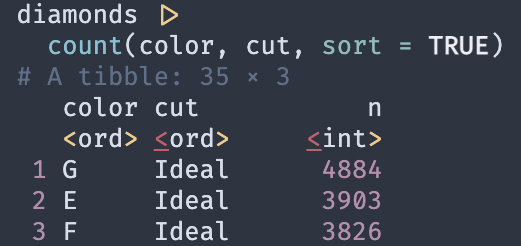
\includegraphics[keepaspectratio]{media/nord-mistake.png}}

I could copy over the \texttt{.theme} file and modify it in the right
place, but I'm lazy and modify it directly in the \texttt{.scss} file
instead by adding which will fix the color and remove the underline

\begin{Shaded}
\begin{Highlighting}[]
\NormalTok{code span}\FunctionTok{.er}\NormalTok{ \{}
  \KeywordTok{color}\NormalTok{: }\ConstantTok{\#ebcb8b}\OperatorTok{;}
  \KeywordTok{text{-}decoration}\NormalTok{: }\DecValTok{none}\OperatorTok{;}
\NormalTok{\}}
\end{Highlighting}
\end{Shaded}

The line numbers are not too important this code chunk so I set
\texttt{\#\textbar{}\ code-line-numbers:\ false}. Then I start working
on styling the source div.

\begin{Shaded}
\begin{Highlighting}[]
\FunctionTok{.reveal}\NormalTok{ div}\FunctionTok{.sourceCode}\NormalTok{ \{}
  \KeywordTok{border}\NormalTok{: }\DecValTok{none}\OperatorTok{;}
  \KeywordTok{border{-}radius}\NormalTok{: }\DecValTok{5}\DataTypeTok{px}\OperatorTok{;}
  \KeywordTok{margin{-}bottom}\NormalTok{: }\DecValTok{10}\DataTypeTok{px} \AttributeTok{!important}\OperatorTok{;}
  \KeywordTok{box{-}shadow}\NormalTok{: }\DecValTok{0} \DecValTok{20}\DataTypeTok{px} \DecValTok{47}\DataTypeTok{px} \FunctionTok{rgb(}\DecValTok{0} \DecValTok{0} \DecValTok{0} \OperatorTok{/} \DecValTok{55}\DataTypeTok{\%}\FunctionTok{)}\OperatorTok{;}
  \KeywordTok{width}\NormalTok{: }\DecValTok{fit{-}content}\OperatorTok{;}
  \KeywordTok{margin}\NormalTok{: }\BuiltInTok{auto} \AttributeTok{!important}\OperatorTok{;}
\NormalTok{\}}
\end{Highlighting}
\end{Shaded}

The main thing that changes is that I brought back the
\texttt{border-radius}. I added some \texttt{box-shadow}s. These things
alone make a huge difference in appearance.

Next, I changed \texttt{width:\ fit-content;}, this makes it so the
width of the div changes with the width of the code, the code I have
right now isn't that wide and it looked a little lopsided. Lastly, I set
\texttt{margin:\ auto\ !important;}, which centers the div so it doesn't
cling to the left side.

The very final thing I changed is adding some padding to the code, this
is the space between the code itself and the inside border of the div, I
did this by adding

\begin{Shaded}
\begin{Highlighting}[]
\FunctionTok{.reveal}\NormalTok{ div}\FunctionTok{.sourceCode}\NormalTok{ pre code \{}
  \KeywordTok{padding}\NormalTok{: }\DecValTok{25}\DataTypeTok{px}\OperatorTok{;}
\NormalTok{\}}
\end{Highlighting}
\end{Shaded}

All of this results in the following slide:

\pandocbounded{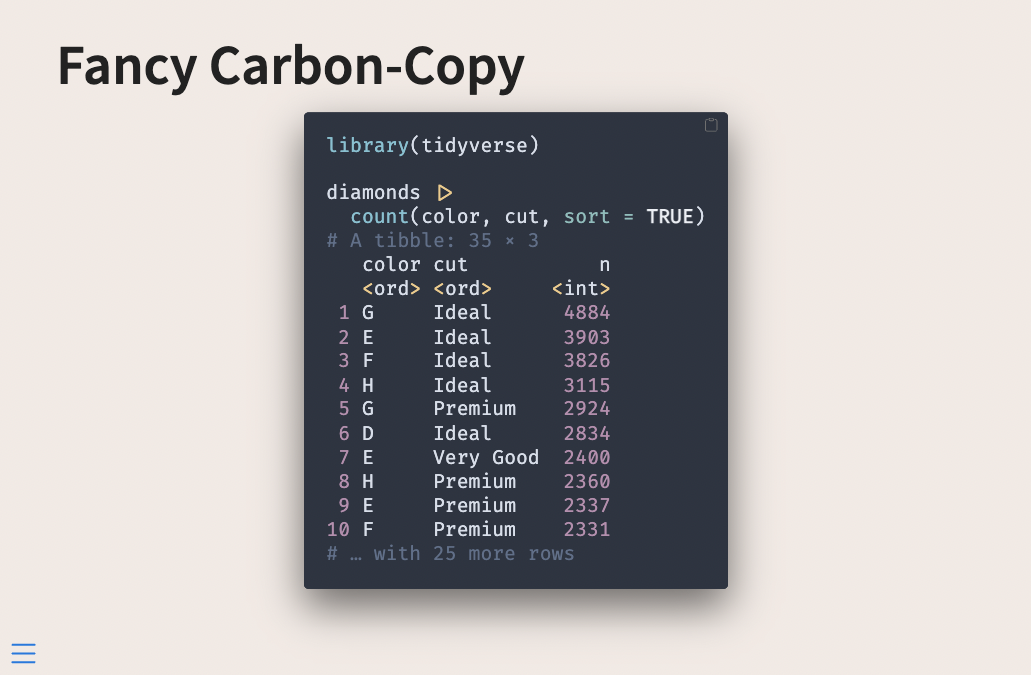
\includegraphics[keepaspectratio]{media/carbon-copy.png}}

\section{Style menu button}\label{style-menu-button}

The menu button you see in the lower left-hand side of the slide.
Styling it can be done by setting the \texttt{\$link-color} sass
variable. If you want a different icon, or have it colored differently
than \texttt{\$link-color} you need to specify it directly as the color
\href{https://github.com/quarto-dev/quarto-cli/blob/13c916d041b2f83c20855fd24c7bd68d07720981/src/resources/formats/revealjs/quarto.scss\#L505}{is
hardcoded into the svg}. The icon is specified as the background image
of \texttt{.reveal\ .slide-menu-button\ .fa-bars::before}.

\begin{Shaded}
\begin{Highlighting}[]
\FunctionTok{.reveal} \FunctionTok{.slide{-}menu{-}button} \FunctionTok{.fa{-}bars}\InformationTok{::before}\NormalTok{ \{}
\KeywordTok{background{-}image}\NormalTok{: }\FunctionTok{url(}\StringTok{\textquotesingle{}data:image/svg+xml,\textless{}svg xmlns="http://www.w3.org/2000/svg" width="16" height="16" fill="rgb(42, 118, 221)" class="bi bi{-}list" viewBox="0 0 16 16"\textgreater{}\textless{}path fill{-}rule="evenodd" d="M2.5 12a.5.5 0 0 1 .5{-}.5h10a.5.5 0 0 1 0 1H3a.5.5 0 0 1{-}.5{-}.5zm0{-}4a.5.5 0 0 1 .5{-}.5h10a.5.5 0 0 1 0 1H3a.5.5 0 0 1{-}.5{-}.5zm0{-}4a.5.5 0 0 1 .5{-}.5h10a.5.5 0 0 1 0 1H3a.5.5 0 0 1{-}.5{-}.5z"/\textgreater{}\textless{}/svg\textgreater{}\textquotesingle{}}\FunctionTok{)} \AttributeTok{!important}\OperatorTok{;}
\NormalTok{\}}
\end{Highlighting}
\end{Shaded}

Tthe color is specified by the \texttt{fill="rgb(42,\ 118,\ 221)"} part
of the svg. But since this is an image, we can use whatever image we
want.

\begin{Shaded}
\begin{Highlighting}[]
\FunctionTok{.reveal} \FunctionTok{.slide{-}menu{-}button} \FunctionTok{.fa{-}bars}\InformationTok{::before}\NormalTok{ \{}
\KeywordTok{background{-}image}\NormalTok{: }\FunctionTok{url(}\StringTok{\textquotesingle{}https://cdn{-}icons{-}png.flaticon.com/512/2163/2163350.png\textquotesingle{}}\FunctionTok{)} \AttributeTok{!important}\OperatorTok{;}
\NormalTok{\}}
\end{Highlighting}
\end{Shaded}

\faIcon{file}qmd \faIcon{sass}scss

\chapter{SCSS}\label{scss}

\section{\texorpdfstring{Using \texttt{Maps} to store theme
colors}{Using Maps to store theme colors}}\label{using-maps-to-store-theme-colors}

Before I would have specified a color palette theme as

\begin{Shaded}
\begin{Highlighting}[]
\VariableTok{$theme{-}red}\NormalTok{: }\ConstantTok{\#FA5F5C}\OperatorTok{;}
\VariableTok{$theme{-}blue}\NormalTok{: }\ConstantTok{\#394D85}\OperatorTok{;}
\VariableTok{$theme{-}darkblue}\NormalTok{: }\ConstantTok{\#13234B}\OperatorTok{;}
\VariableTok{$theme{-}yellow}\NormalTok{: }\ConstantTok{\#FFF7C7}\OperatorTok{;}
\VariableTok{$theme{-}white}\NormalTok{: }\ConstantTok{\#FEFEFE}\OperatorTok{;}
\end{Highlighting}
\end{Shaded}

But using a map it turns into the following

\begin{Shaded}
\begin{Highlighting}[]
\VariableTok{$colors}\NormalTok{: (}
  \StringTok{"red"}\NormalTok{: }\ConstantTok{\#FA5F5C}\OperatorTok{,}
  \StringTok{"blue"}\NormalTok{: }\ConstantTok{\#394D85}\OperatorTok{,}
  \StringTok{"darkblue"}\NormalTok{: }\ConstantTok{\#13234B}\OperatorTok{,}
  \StringTok{"yellow"}\NormalTok{: }\ConstantTok{\#FFF7C7}\OperatorTok{,}
  \StringTok{"white"}\NormalTok{: }\ConstantTok{\#FEFEFE}
\NormalTok{)}\OperatorTok{;}
\end{Highlighting}
\end{Shaded}

\begin{tcolorbox}[enhanced jigsaw, titlerule=0mm, bottomrule=.15mm, opacityback=0, colbacktitle=quarto-callout-note-color!10!white, colframe=quarto-callout-note-color-frame, coltitle=black, breakable, toprule=.15mm, colback=white, bottomtitle=1mm, title=\textcolor{quarto-callout-note-color}{\faInfo}\hspace{0.5em}{Note}, toptitle=1mm, arc=.35mm, left=2mm, leftrule=.75mm, rightrule=.15mm, opacitybacktitle=0.6]

There is a difference between \texttt{(key:\ value)} and
\texttt{("key":\ value)} in SASS. For consistency, I also use quoted
strings as the keys in a map.

\end{tcolorbox}

Instead of having multiple values representing our colors we now just
have one \texttt{\$colors}. By themselves, maps aren't valid CSS and
don't do anything once the SASS compiles. The next sections will show
how we can use these maps more efficiently than my previous approach.

\section{\texorpdfstring{Using \texttt{Functions} to pull out theme
colors}{Using Functions to pull out theme colors}}\label{using-functions-to-pull-out-theme-colors}

We where using these colors to change a lot of things, including the
major
\href{https://quarto.org/docs/presentations/revealjs/themes.html\#sass-variables}{Sass
Variables} revealjs sass variables. Before we used a map, it would look
something like this:

\begin{Shaded}
\begin{Highlighting}[]
\VariableTok{$body{-}bg}\NormalTok{: }\VariableTok{$theme{-}yellow}\OperatorTok{;}
\VariableTok{$link{-}color}\NormalTok{: }\VariableTok{$theme{-}blue}\OperatorTok{;}
\VariableTok{$code{-}color}\NormalTok{: }\VariableTok{$theme{-}blue}\OperatorTok{;}
\VariableTok{$body{-}color}\NormalTok{: }\VariableTok{$theme{-}darkblue}\OperatorTok{;}
\end{Highlighting}
\end{Shaded}

but we can't do that directly with a map. There are built-in functions
to extract values from a map, namely the function
\href{https://sass-lang.com/documentation/values/maps/\#look-up-a-value}{map-get()}.
Using that we can rewrite the above as

\begin{Shaded}
\begin{Highlighting}[]
\VariableTok{$body{-}bg}\NormalTok{: }\FunctionTok{map{-}get(}\VariableTok{$colors}\OperatorTok{,} \StringTok{"yellow"}\FunctionTok{)}\OperatorTok{;}
\VariableTok{$link{-}color}\NormalTok{: }\FunctionTok{map{-}get(}\VariableTok{$colors}\OperatorTok{,} \StringTok{"blue"}\FunctionTok{)}\OperatorTok{;}
\VariableTok{$code{-}color}\NormalTok{: }\FunctionTok{map{-}get(}\VariableTok{$colors}\OperatorTok{,} \StringTok{"blue"}\FunctionTok{)}\OperatorTok{;}
\VariableTok{$body{-}color}\NormalTok{: }\FunctionTok{map{-}get(}\VariableTok{$colors}\OperatorTok{,} \StringTok{"darkblue"}\FunctionTok{)}\OperatorTok{;}
\end{Highlighting}
\end{Shaded}

And while that is all good, I find it a little nicer to have a helper
\href{https://sass-lang.com/documentation/at-rules/function/}{function}
to do this.

Functions in SASS are written as below. You can use as many arguments as
you want.

\begin{Shaded}
\begin{Highlighting}[]
\ImportTok{@function} \FunctionTok{name}\NormalTok{(}\VariableTok{$arg1}\OperatorTok{,} \VariableTok{$arg2}\NormalTok{) \{}
  \ImportTok{@return} \VariableTok{$arg1} \OperatorTok{+} \VariableTok{$arg2}\OperatorTok{;}
\NormalTok{\}}
\end{Highlighting}
\end{Shaded}

The helper function I wrote is a light wrapper around \texttt{map-get()}
to avoid having to write \texttt{\$colors}.

\begin{Shaded}
\begin{Highlighting}[]
\ImportTok{@function} \FunctionTok{theme{-}color}\NormalTok{(}\VariableTok{$color}\NormalTok{) \{}
  \ImportTok{@return} \FunctionTok{map{-}get(}\VariableTok{$colors}\OperatorTok{,} \VariableTok{$color}\FunctionTok{)}\OperatorTok{;}
\NormalTok{\}}
\end{Highlighting}
\end{Shaded}

And we now have the final rewrite.

\begin{Shaded}
\begin{Highlighting}[]
\VariableTok{$body{-}bg}\NormalTok{: }\FunctionTok{theme{-}color(}\StringTok{"yellow"}\FunctionTok{)}\OperatorTok{;}
\VariableTok{$link{-}color}\NormalTok{: }\FunctionTok{theme{-}color(}\StringTok{"blue"}\FunctionTok{)}\OperatorTok{;}
\VariableTok{$code{-}color}\NormalTok{: }\FunctionTok{theme{-}color(}\StringTok{"blue"}\FunctionTok{)}\OperatorTok{;}
\VariableTok{$body{-}color}\NormalTok{: }\FunctionTok{theme{-}color(}\StringTok{"darkblue"}\FunctionTok{)}\OperatorTok{;}
\end{Highlighting}
\end{Shaded}

\begin{tcolorbox}[enhanced jigsaw, titlerule=0mm, bottomrule=.15mm, opacityback=0, colbacktitle=quarto-callout-note-color!10!white, colframe=quarto-callout-note-color-frame, coltitle=black, breakable, toprule=.15mm, colback=white, bottomtitle=1mm, title=\textcolor{quarto-callout-note-color}{\faInfo}\hspace{0.5em}{Note}, toptitle=1mm, arc=.35mm, left=2mm, leftrule=.75mm, rightrule=.15mm, opacitybacktitle=0.6]

Note that we are using \texttt{theme-color("yellow")} instead of
\texttt{theme-color(yellow)} because we used quoted strings in the map.
Using unquoted strings all around gave me false positives in my IDE as
it interpreted \texttt{yellow} inside \texttt{theme-color()} as
\texttt{\#FFFF00} instead of my theme value.

\end{tcolorbox}

\section{\texorpdfstring{Using \texttt{@each} to automatically create
classes}{Using @each to automatically create classes}}\label{using-each-to-automatically-create-classes}

To add a splash of color, or as used in highlighting, I would create a
lot of CSS classes like so:

\begin{Shaded}
\begin{Highlighting}[]
\FunctionTok{.text{-}red}\NormalTok{ \{}
  \KeywordTok{color}\NormalTok{: }\VariableTok{$theme{-}red}\OperatorTok{;}
\NormalTok{\}}
\FunctionTok{.text{-}yellow}\NormalTok{ \{}
  \KeywordTok{color}\NormalTok{: }\VariableTok{$theme{-}yellow}\OperatorTok{;}
\NormalTok{\}}
\FunctionTok{.text{-}blue}\NormalTok{ \{}
  \KeywordTok{color}\NormalTok{: }\VariableTok{$theme{-}blue}\OperatorTok{;}
\NormalTok{\}}

\FunctionTok{.bg{-}red}\NormalTok{ \{}
  \KeywordTok{background{-}color}\NormalTok{: }\VariableTok{$theme{-}red}\OperatorTok{;}
\NormalTok{\}}
\FunctionTok{.bg{-}yellow}\NormalTok{ \{}
  \KeywordTok{background{-}color}\NormalTok{: }\VariableTok{$theme{-}yellow}\OperatorTok{;}
\NormalTok{\}}
\FunctionTok{.bg{-}blue}\NormalTok{ \{}
  \KeywordTok{background{-}color}\NormalTok{: }\VariableTok{$theme{-}blue}\OperatorTok{;}
\NormalTok{\}}
\end{Highlighting}
\end{Shaded}

Which is all fine and dandy until you also want a class for underlining.
It becomes a lot of copy-pasting and changing a couple of names. And
that is not to mention the trouble you run into when you decide to add a
new color into the mix halfway through your slides.

This is when I discovered
\href{https://sass-lang.com/documentation/interpolation/}{interpolation}
and the moment I realized maps were worth it. Interpolation is done by
using \texttt{\#\{\}} in some code, meaning that if
\texttt{\$favorite-color:\ "blue"} then
\texttt{.text-\#\{\$favorite-color\}\ \{\}} turns into
\texttt{.text-blue\ \{\}}. SASS provides the action
\href{https://sass-lang.com/documentation/at-rules/control/each/}{\texttt{@each}}
to loop over all the key and value pairs of our map. So we can rewrite
the creation of the above classes as this:

\begin{Shaded}
\begin{Highlighting}[]
\ImportTok{@each} \VariableTok{$name}\NormalTok{, }\VariableTok{$color}\NormalTok{ in }\VariableTok{$colors}\NormalTok{ \{}
  \FunctionTok{.text{-}}\OperatorTok{\#\{}\VariableTok{$name}\OperatorTok{\}}\NormalTok{ \{}
    \KeywordTok{color}\NormalTok{: }\VariableTok{$color}\OperatorTok{;}
\NormalTok{  \}}

  \FunctionTok{.bg{-}}\OperatorTok{\#\{}\VariableTok{$name}\OperatorTok{\}}\NormalTok{ \{}
    \KeywordTok{background{-}color}\NormalTok{: }\VariableTok{$color}\OperatorTok{;}
\NormalTok{  \}}
\NormalTok{\}}
\end{Highlighting}
\end{Shaded}

And this is the beauty of maps. If I want to add a new color to my
slides, I just have to add it to the \texttt{\$colors} map. If I want to
add a new set of classes, I just have to write it once inside the
\texttt{@each} statement.

\section{\texorpdfstring{Using \texttt{@mixin} to avoid repeating
code}{Using @mixin to avoid repeating code}}\label{using-mixin-to-avoid-repeating-code}

With the following code

\begin{Shaded}
\begin{Highlighting}[]
\ImportTok{@mixin} \FunctionTok{background{-}full}\NormalTok{ \{}
  \KeywordTok{background{-}size}\NormalTok{: }\DecValTok{cover}\OperatorTok{;}
  \KeywordTok{background{-}position}\NormalTok{: }\DecValTok{center}\OperatorTok{;}
  \KeywordTok{background{-}repeat}\NormalTok{: }\DecValTok{no{-}repeat}\OperatorTok{;}
\NormalTok{\}}

\FunctionTok{.theme{-}slide1}\NormalTok{ \{}
  \OperatorTok{\&}\InformationTok{:is(.slide{-}background)}\NormalTok{ \{}
    \KeywordTok{background{-}image}\NormalTok{: }\FunctionTok{url(}\StringTok{\textquotesingle{}../../../../../assets/slide1.svg\textquotesingle{}}\FunctionTok{)}\OperatorTok{;}
    \ImportTok{@include}\NormalTok{ background{-}full}\OperatorTok{;}
\NormalTok{  \}}
\NormalTok{\}}
\FunctionTok{.theme{-}slide2}\NormalTok{ \{}
  \OperatorTok{\&}\InformationTok{:is(.slide{-}background)}\NormalTok{ \{}
    \KeywordTok{background{-}image}\NormalTok{: }\FunctionTok{url(}\StringTok{\textquotesingle{}../../../../../assets/slide2.svg\textquotesingle{}}\FunctionTok{)}\OperatorTok{;}
    \ImportTok{@include}\NormalTok{ background{-}full}\OperatorTok{;}
\NormalTok{  \}}
\NormalTok{\}}
\FunctionTok{.theme{-}slide3}\NormalTok{ \{}
  \OperatorTok{\&}\InformationTok{:is(.slide{-}background)}\NormalTok{ \{}
    \KeywordTok{background{-}image}\NormalTok{: }\FunctionTok{url(}\StringTok{\textquotesingle{}../../../../../assets/slide3.svg\textquotesingle{}}\FunctionTok{)}\OperatorTok{;}
    \ImportTok{@include}\NormalTok{ background{-}full}\OperatorTok{;}
\NormalTok{  \}}
\NormalTok{\}}
\end{Highlighting}
\end{Shaded}

Copy-pasting this around when you have 10-15 images is such a pain. But
as you properly have noticed, interpolation would be a perfect solution
to this problem, and you would be correct! We use a
\href{https://sass-lang.com/documentation/at-rules/mixin/}{\texttt{@mixin}}
to create to create a way to create many classes:

\begin{Shaded}
\begin{Highlighting}[]
\ImportTok{@mixin} \FunctionTok{theme{-}slide}\NormalTok{(}\VariableTok{$number}\NormalTok{) \{}
  \FunctionTok{.theme{-}slide}\OperatorTok{\#\{}\VariableTok{$number}\OperatorTok{\}}\NormalTok{ \{}
    \OperatorTok{\&}\InformationTok{:is(.slide{-}background)}\NormalTok{ \{}
      \KeywordTok{background{-}image}\NormalTok{: }\FunctionTok{url(}\StringTok{\textquotesingle{}../../../../../assets/slide}\OperatorTok{\#\{}\VariableTok{$number}\OperatorTok{\}}\StringTok{.svg\textquotesingle{}}\FunctionTok{)}\OperatorTok{;}
      \ImportTok{@include}\NormalTok{ background{-}full}\OperatorTok{;}
\NormalTok{    \}}
\NormalTok{  \}}
\NormalTok{\}}

\ImportTok{@include} \FunctionTok{theme{-}slide(}\DecValTok{1}\FunctionTok{)}\OperatorTok{;}
\ImportTok{@include} \FunctionTok{theme{-}slide(}\DecValTok{2}\FunctionTok{)}\OperatorTok{;}
\ImportTok{@include} \FunctionTok{theme{-}slide(}\DecValTok{3}\FunctionTok{)}\OperatorTok{;}
\end{Highlighting}
\end{Shaded}

It becomes quite a bit tighter! But we can do better because SASS also
has
\href{https://sass-lang.com/documentation/at-rules/control/for/}{\texttt{@for}}
loops.

\begin{Shaded}
\begin{Highlighting}[]
\ImportTok{@mixin} \FunctionTok{theme{-}slide}\NormalTok{(}\VariableTok{$number}\NormalTok{) \{}
  \FunctionTok{.theme{-}slide}\OperatorTok{\#\{}\VariableTok{$number}\OperatorTok{\}}\NormalTok{ \{}
    \OperatorTok{\&}\InformationTok{:is(.slide{-}background)}\NormalTok{ \{}
      \KeywordTok{background{-}image}\NormalTok{: }\FunctionTok{url(}\StringTok{\textquotesingle{}../../../../../assets/slide}\OperatorTok{\#\{}\VariableTok{$number}\OperatorTok{\}}\StringTok{.svg\textquotesingle{}}\FunctionTok{)}\OperatorTok{;}
      \ImportTok{@include}\NormalTok{ background{-}full}\OperatorTok{;}
\NormalTok{    \}}
\NormalTok{  \}}
\NormalTok{\}}

\ImportTok{@for} \VariableTok{$i}\NormalTok{ from }\DecValTok{1}\NormalTok{ through }\DecValTok{3}\NormalTok{ \{}
  \ImportTok{@include} \FunctionTok{theme{-}slide(}\VariableTok{$i}\FunctionTok{)}\OperatorTok{;}
\NormalTok{\}}
\end{Highlighting}
\end{Shaded}

you can now add more background images with ease as long as you are
careful when naming them.

\section{Using nested loops to create
classes}\label{using-nested-loops-to-create-classes}

In our first example, I want a fun gradient shadow/highlight effect for
text. We can get that effect using something like following

\begin{Shaded}
\begin{Highlighting}[]
\NormalTok{background{-}image}\InformationTok{:}\NormalTok{ linear{-}gradient}\InformationTok{(}\NormalTok{90deg}\OperatorTok{,}\NormalTok{ yellow}\OperatorTok{,}\NormalTok{ blue}\InformationTok{)}\NormalTok{;}
\NormalTok{background{-}size}\InformationTok{:}\NormalTok{ 100\% 42\%;}
\NormalTok{background{-}repeat}\InformationTok{:}\NormalTok{ no{-}repeat;}
\NormalTok{background{-}position}\InformationTok{:}\NormalTok{ 0 85\%;}
\NormalTok{width}\InformationTok{:}\NormalTok{ fit{-}content;}
\end{Highlighting}
\end{Shaded}

I want it to work on both inline text and as a way to handle the header,
the selectors for that would be \texttt{span.my-class} and
\texttt{.my-class\ \textgreater{}\ h2} respectively.

\begin{Shaded}
\begin{Highlighting}[]
\NormalTok{span}\FunctionTok{.my{-}class}\OperatorTok{,} \FunctionTok{.my{-}class} \OperatorTok{\textgreater{}}\NormalTok{ h2 \{}
  \KeywordTok{background{-}image}\CharTok{:} \FunctionTok{linear{-}gradient(}\DecValTok{90}\DataTypeTok{deg}\OperatorTok{,} \ConstantTok{yellow}\OperatorTok{,} \ConstantTok{blue}\FunctionTok{)}\OperatorTok{;}
  \KeywordTok{background{-}size}\CharTok{:} \DecValTok{100}\DataTypeTok{\%} \DecValTok{42}\DataTypeTok{\%}\OperatorTok{;}
  \KeywordTok{background{-}repeat}\CharTok{:} \DecValTok{no{-}repeat}\OperatorTok{;}
  \KeywordTok{background{-}position}\CharTok{:} \DecValTok{0} \DecValTok{85}\DataTypeTok{\%}\OperatorTok{;}
  \KeywordTok{width}\CharTok{:} \DecValTok{fit{-}content}\OperatorTok{;}
\NormalTok{\}}
\end{Highlighting}
\end{Shaded}

And them we fill in the rest, using the
\href{https://sass-lang.com/documentation/at-rules/control/each/\#with-maps}{\texttt{@each}}
command twice nestedly over a map of colors.

\begin{Shaded}
\begin{Highlighting}[]
\CommentTok{/*{-}{-} scss:defaults {-}{-}*/}

\VariableTok{$colors}\NormalTok{: (}
  \StringTok{"red"}\NormalTok{: }\ConstantTok{\#FFADAD}\OperatorTok{,} 
\StringTok{"orange"}\NormalTok{: }\ConstantTok{\#FFD6A5}\OperatorTok{,} 
  \StringTok{"yellow"}\NormalTok{: }\ConstantTok{\#FDFFB6}\OperatorTok{,} 
  \StringTok{"blue"}\NormalTok{: }\ConstantTok{\#aad2e7}\OperatorTok{,} 
  \StringTok{"purple"}\NormalTok{:}\ConstantTok{\#b4addd}
\NormalTok{)}\OperatorTok{;}

\CommentTok{/*{-}{-} scss:rules {-}{-}*/}

\ImportTok{@each} \VariableTok{$name1}\NormalTok{, }\VariableTok{$col1}\NormalTok{ in }\VariableTok{$colors}\NormalTok{ \{}
  \ImportTok{@each} \VariableTok{$name2}\NormalTok{, }\VariableTok{$col2}\NormalTok{ in }\VariableTok{$colors}\NormalTok{ \{}
\NormalTok{    span}\FunctionTok{.hl{-}}\OperatorTok{\#\{}\VariableTok{$name1}\OperatorTok{\}}\NormalTok{{-}}\OperatorTok{\#\{}\VariableTok{$name2}\OperatorTok{\},} \FunctionTok{.hl{-}}\OperatorTok{\#\{}\VariableTok{$name1}\OperatorTok{\}}\NormalTok{{-}}\OperatorTok{\#\{}\VariableTok{$name2}\OperatorTok{\}} \OperatorTok{\textgreater{}}\NormalTok{ h2 \{}
      \KeywordTok{background{-}image}\NormalTok{: }\FunctionTok{linear{-}gradient(}\DecValTok{90}\DataTypeTok{deg}\OperatorTok{,} \VariableTok{$col1}\OperatorTok{,} \VariableTok{$col2}\FunctionTok{)}\OperatorTok{;}
      \KeywordTok{background{-}size}\NormalTok{: }\DecValTok{100}\DataTypeTok{\%} \DecValTok{42}\DataTypeTok{\%}\OperatorTok{;}
      \KeywordTok{background{-}repeat}\NormalTok{: }\DecValTok{no{-}repeat}\OperatorTok{;}
      \KeywordTok{background{-}position}\NormalTok{: }\DecValTok{0} \DecValTok{85}\DataTypeTok{\%}\OperatorTok{;}
      \KeywordTok{width}\NormalTok{: }\DecValTok{fit{-}content}\OperatorTok{;}
\NormalTok{    \}}
\NormalTok{  \}}
\NormalTok{\}}
\end{Highlighting}
\end{Shaded}

I know we are creating some non-interesting classes such as
\texttt{.hl-yellow-yellow} but for what we are doing, the tradeoff
between avoiding them and how little it impacts us to have them. I think
it is a worthwhile tradeoff.

\begin{tcolorbox}[enhanced jigsaw, titlerule=0mm, bottomrule=.15mm, opacityback=0, colbacktitle=quarto-callout-important-color!10!white, colframe=quarto-callout-important-color-frame, coltitle=black, breakable, toprule=.15mm, colback=white, bottomtitle=1mm, title=\textcolor{quarto-callout-important-color}{\faExclamation}\hspace{0.5em}{Important}, toptitle=1mm, arc=.35mm, left=2mm, leftrule=.75mm, rightrule=.15mm, opacitybacktitle=0.6]

The slides in this post are interactive, advance them to see the other
classes.

\end{tcolorbox}

\faIcon{file}qmd \faIcon{sass}scss

\begin{tcolorbox}[enhanced jigsaw, titlerule=0mm, bottomrule=.15mm, opacityback=0, colbacktitle=quarto-callout-note-color!10!white, colframe=quarto-callout-note-color-frame, coltitle=black, breakable, toprule=.15mm, colback=white, bottomtitle=1mm, title=\textcolor{quarto-callout-note-color}{\faInfo}\hspace{0.5em}{Note}, toptitle=1mm, arc=.35mm, left=2mm, leftrule=.75mm, rightrule=.15mm, opacitybacktitle=0.6]

You don't need these compound classes for everything. For example, the
class \texttt{.hl-green-bold} isn't going to be useful as you could just
as easily create \texttt{.hl-green} and \texttt{.bold} separately. This
trick works best when two elements are used together in a tightly
coupled way, such as in gradients.

\end{tcolorbox}

For our second example, we are continuing with the gradients, but
instead trying to apply them to the background. My goal was to add a
gradient line to the right side of the slide.

I was able to create that effect, by layering 2 gradients on top of each
other. The first gradient contained the two colors I was interested in,
and the names of the class. The second layer, which I placed on top,
goes from white to transparent. I set up the transition between those
two colors to be super sharp, resulting in the effect you see below

\faIcon{file}qmd \faIcon{sass}scss

since we are doing something interesting, we could also have used a
separate \texttt{\$colors} map just for this effect to not interfere
with what else we are doing.

\part{Content}

\chapter{Elements}\label{elements}

\section{Showing quarto code}\label{showing-quarto-code}

This one isn't as much a slidecrafting tip, as it is a quarto tip! If
you are showing how to do something in Quarto using Quarto you need this
tip. In essence what we are working with are
\href{https://quarto.org/docs/computations/execution-options.html\#unexecuted-blocks}{unexcuted
blocks}.

Adding a \texttt{markdown} cell around what you want to show. Important
to use more ticks than any of the inside cells inside

using double curly brackets to indicate that the code block should not
be executed. The following code when used in a quarto document will
render as shown in the example

\begin{Shaded}
\begin{Highlighting}[]
\InformationTok{\textasciigrave{}\textasciigrave{}\textasciigrave{}\textasciigrave{} markdown}
\NormalTok{This is **Quarto** code}

\InformationTok{\textasciigrave{}\textasciigrave{}\textasciigrave{}\{\{python\}\}}
\InformationTok{1 + 1}
\InformationTok{\textasciigrave{}\textasciigrave{}\textasciigrave{}}
\InformationTok{\textasciigrave{}\textasciigrave{}\textasciigrave{}\textasciigrave{}}
\end{Highlighting}
\end{Shaded}

\faIcon{file}qmd

\section{Changing plot backgrounds}\label{changing-plot-backgrounds}

Plots and charts are useful in slides. Changing the background makes
them fit in. This post will go over how to change the background of your
plots to better match the slide background, in a handful of different
libraries.

\subsection{Why are we doing this?}\label{why-are-we-doing-this}

If you are styling your slides to change the background color, you will
find that most plotting libraries default to using a white background
color. If your background is non-white it will stick out like a sore
thumb. I find that changing the background color to something
transparent \texttt{\#FFFFFF00} is the easiest course of action.

\begin{quote}
Why make the background transparent instead of making it match the
background?
\end{quote}

It is simply easier that way. There is only one color we need to set and
it is \texttt{\#FFFFFF00}. This works even if the slide background color
is different from slide to slide, or if the background is a non-solid
color.

\subsection{base R}\label{base-r}

we don't have to make any changes to the R code, we can supply the chunk
options \texttt{dev} and \texttt{dev.args} for the chunk to
\texttt{"png"} and \texttt{list(bg="transparent")} respectively and you
are good. The chunk will look like this.

\begin{Shaded}
\begin{Highlighting}[]
\InformationTok{\textasciigrave{}\textasciigrave{}\textasciigrave{}\{r, dev = "png", dev.args=list(bg="transparent")\}}
\InformationTok{plot(mpg \textasciitilde{} disp, data = mtcars, col = factor(am), pch = 16, bty = "n")}
\InformationTok{\textasciigrave{}\textasciigrave{}\textasciigrave{}}
\end{Highlighting}
\end{Shaded}

You can also change the options globally using the following options in
the yaml.

\begin{Shaded}
\begin{Highlighting}[]
\FunctionTok{knitr}\KeywordTok{:}
\AttributeTok{  }\FunctionTok{opts\_chunk}\KeywordTok{:}
\AttributeTok{    }\FunctionTok{dev}\KeywordTok{:}\AttributeTok{ png}
\AttributeTok{    }\FunctionTok{dev.args}\KeywordTok{:}\AttributeTok{ }\KeywordTok{\{}\AttributeTok{ }\FunctionTok{bg}\KeywordTok{:}\AttributeTok{ }\StringTok{"transparent"}\AttributeTok{ }\KeywordTok{\}}
\end{Highlighting}
\end{Shaded}

\begin{figure}

\begin{minipage}{0.50\linewidth}
\pandocbounded{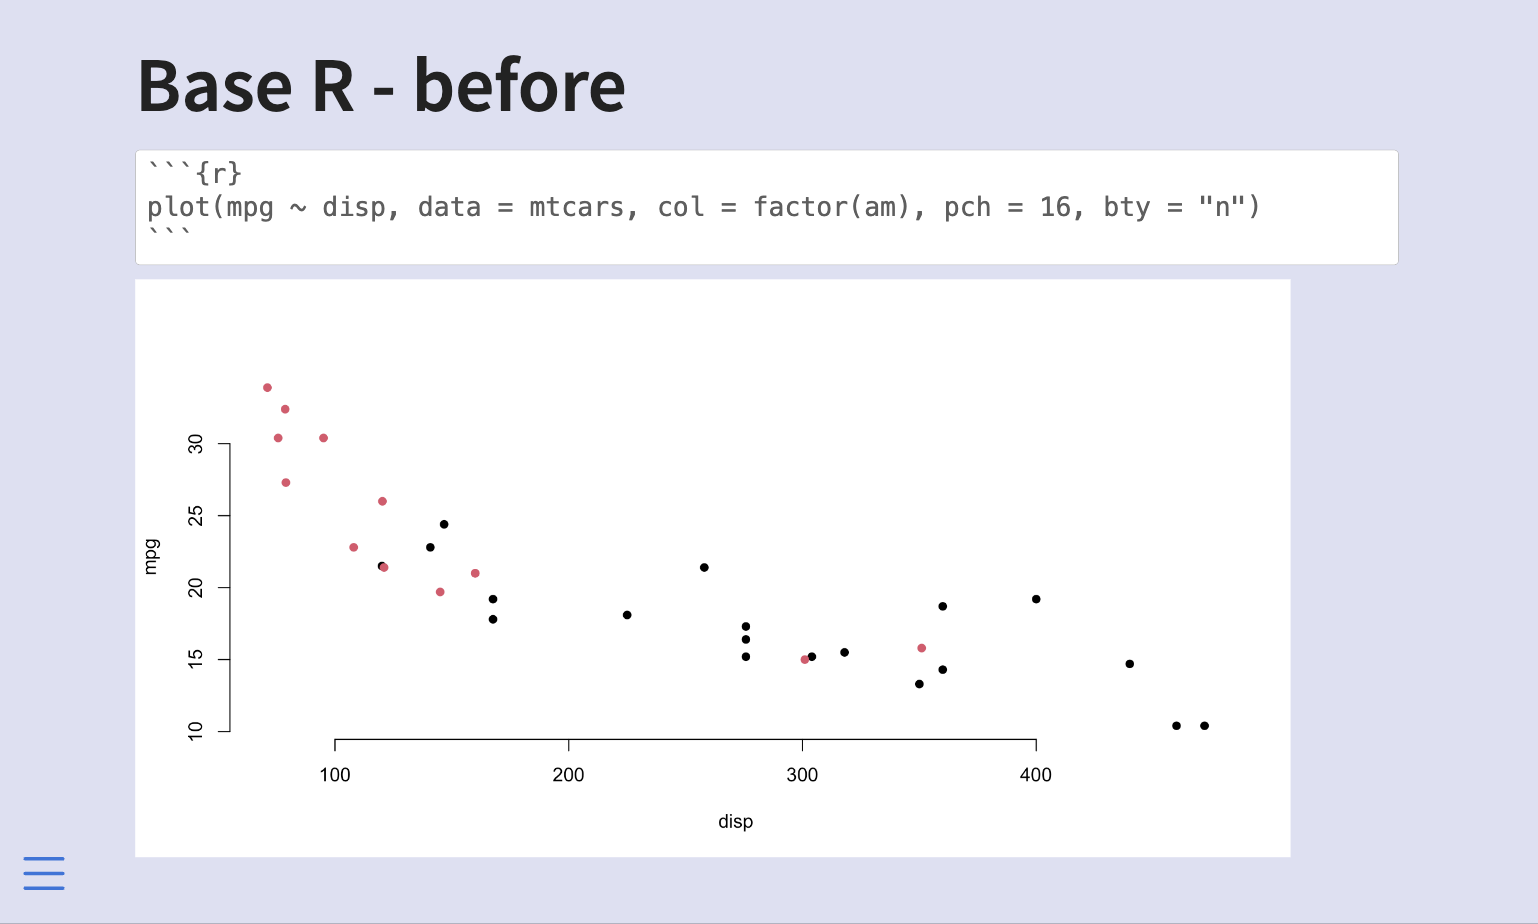
\includegraphics[keepaspectratio]{media/base-before.png}}\end{minipage}%
%
\begin{minipage}{0.50\linewidth}
\pandocbounded{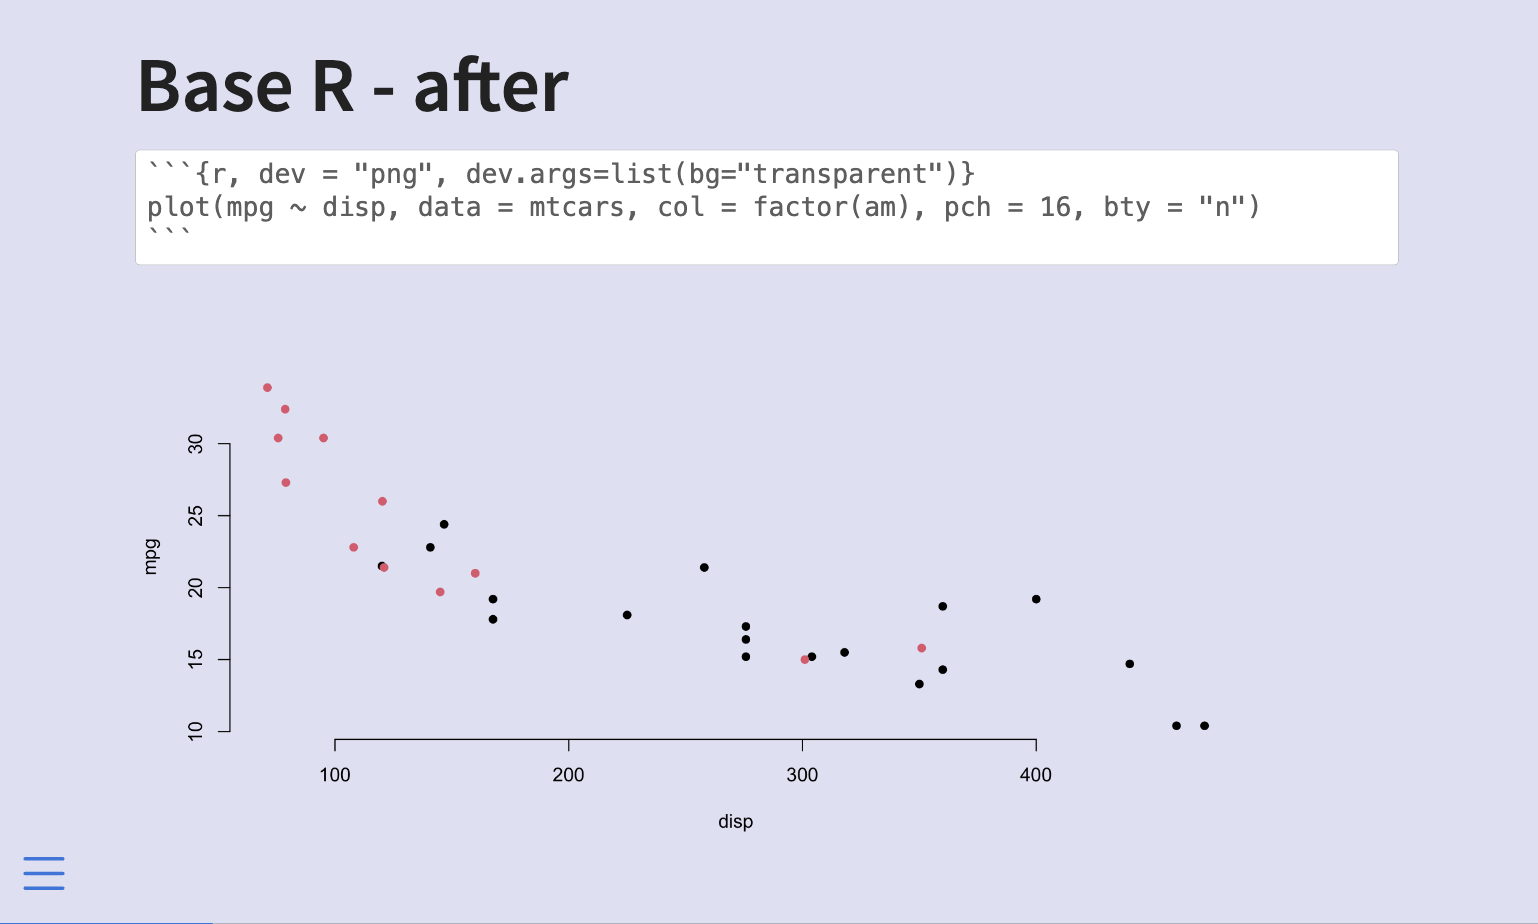
\includegraphics[keepaspectratio]{media/base-after.png}}\end{minipage}%

\end{figure}%

\subsection{ggplot2}\label{ggplot2}

ggplot2 are handled the same way as base R plotting, so we don't have to
make any changes to the R code, we can supply the chunk options
\texttt{dev} and \texttt{dev.args} for the chunk to \texttt{"png"} and
\texttt{list(bg="transparent")} respectively and you are good. The chunk
will look like this.

\begin{Shaded}
\begin{Highlighting}[]
\InformationTok{\textasciigrave{}\textasciigrave{}\textasciigrave{}\{r, dev = "png", dev.args=list(bg="transparent")\}}
\InformationTok{library(ggplot2)}
\InformationTok{mtcars |\textgreater{}}
\InformationTok{  ggplot(aes(disp, mpg, color = factor(am))) +}
\InformationTok{  geom\_point() +}
\InformationTok{  theme\_minimal()}
\InformationTok{\textasciigrave{}\textasciigrave{}\textasciigrave{}}
\end{Highlighting}
\end{Shaded}

You can also change the options globally using the following options in
the yaml.

\begin{Shaded}
\begin{Highlighting}[]
\FunctionTok{knitr}\KeywordTok{:}
\AttributeTok{  }\FunctionTok{opts\_chunk}\KeywordTok{:}
\AttributeTok{    }\FunctionTok{dev}\KeywordTok{:}\AttributeTok{ png}
\AttributeTok{    }\FunctionTok{dev.args}\KeywordTok{:}\AttributeTok{ }\KeywordTok{\{}\AttributeTok{ }\FunctionTok{bg}\KeywordTok{:}\AttributeTok{ }\StringTok{"transparent"}\AttributeTok{ }\KeywordTok{\}}
\end{Highlighting}
\end{Shaded}

\begin{figure}

\begin{minipage}{0.50\linewidth}
\pandocbounded{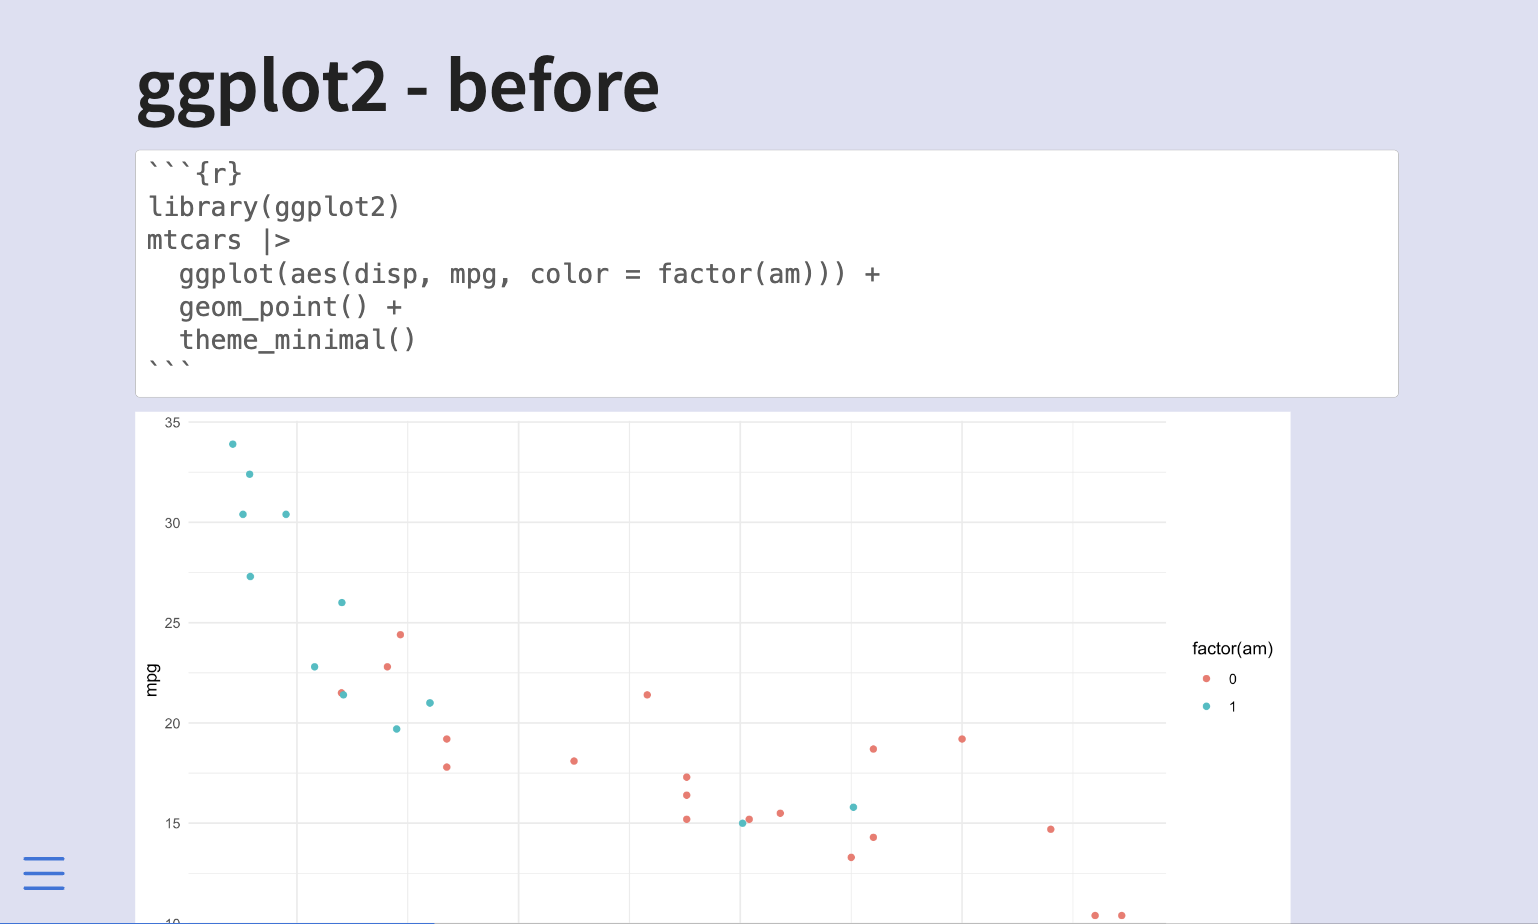
\includegraphics[keepaspectratio]{media/ggplot2-before.png}}\end{minipage}%
%
\begin{minipage}{0.50\linewidth}
\pandocbounded{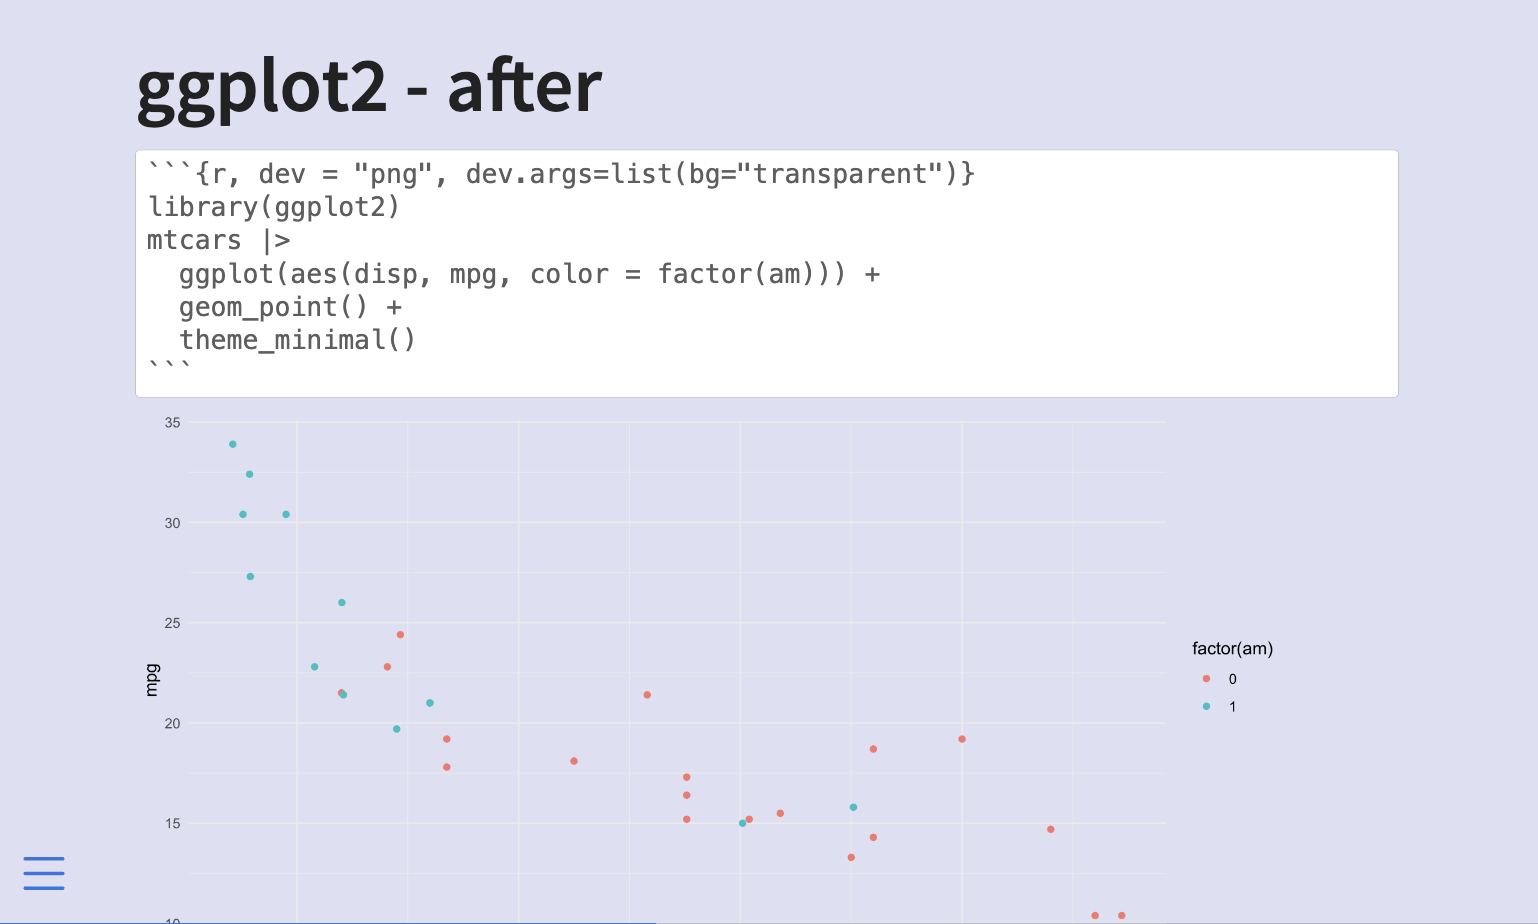
\includegraphics[keepaspectratio]{media/ggplot2-after.png}}\end{minipage}%

\end{figure}%

\subsection{matplotlib}\label{matplotlib}

With matplotlib, we need to set the background color twice, once for the
plotting area, and once for the area outside the plotting area.

\begin{Shaded}
\begin{Highlighting}[]
\NormalTok{fig }\OperatorTok{=}\NormalTok{ plt.figure()}
\CommentTok{\# outside plotting area}
\NormalTok{plt.axes().set\_facecolor(}\StringTok{"\#FFFFFF00"}\NormalTok{)}

\CommentTok{\# your plot}
\NormalTok{plt.scatter(x, y, c}\OperatorTok{=}\NormalTok{colors)}

\CommentTok{\# sinde plotting area}
\NormalTok{fig.patch.set\_facecolor(}\StringTok{"\#FFFFFF00"}\NormalTok{)}
\end{Highlighting}
\end{Shaded}

\begin{figure}

\begin{minipage}{0.50\linewidth}
\pandocbounded{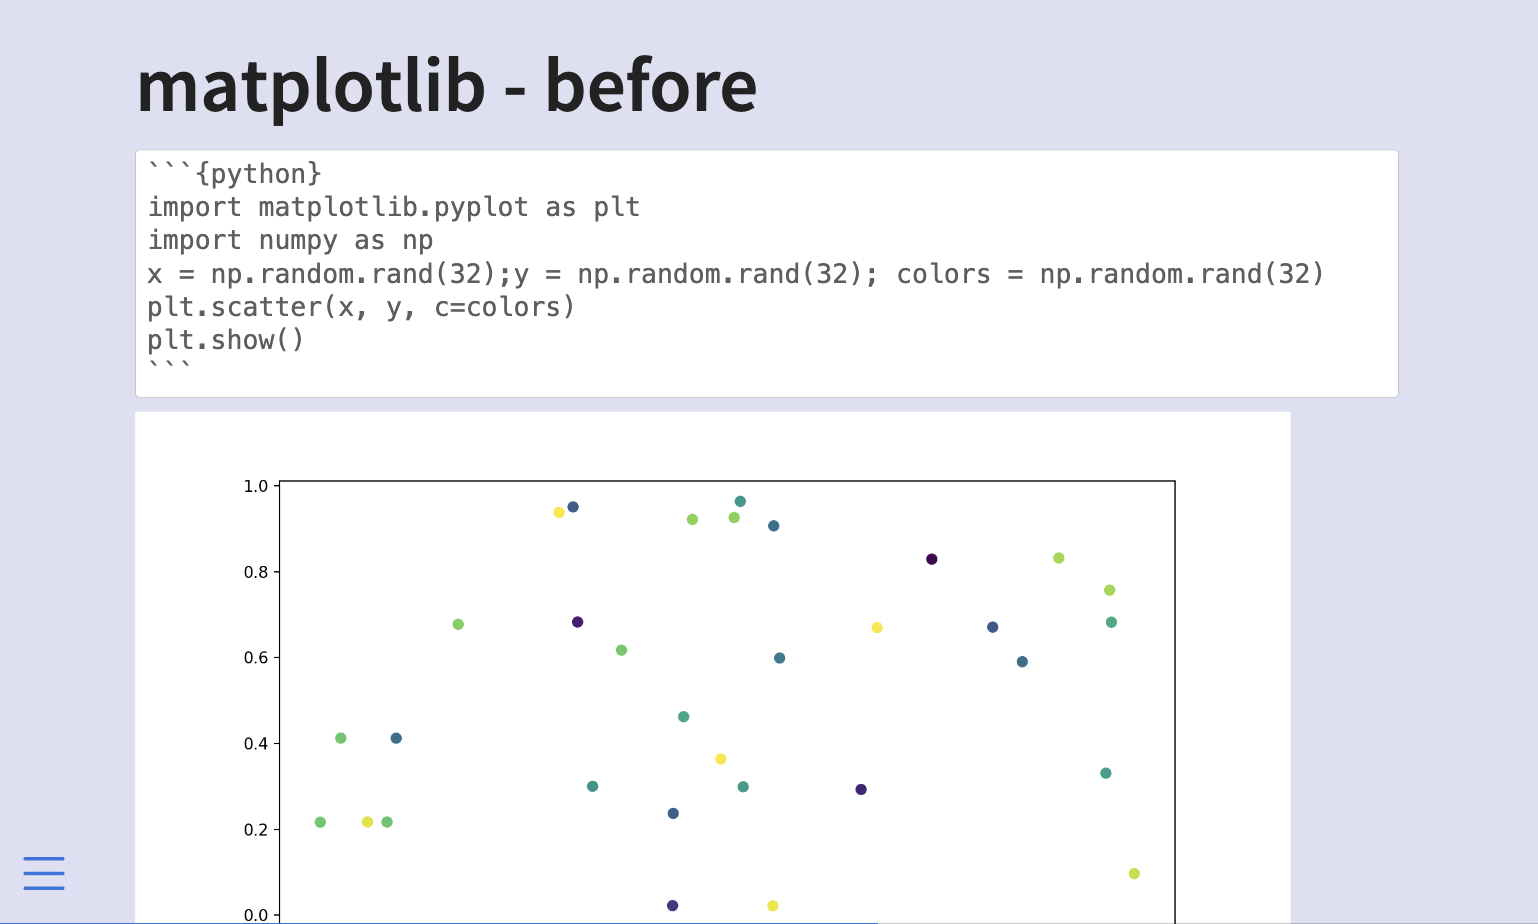
\includegraphics[keepaspectratio]{media/matplotlib-before.png}}\end{minipage}%
%
\begin{minipage}{0.50\linewidth}
\pandocbounded{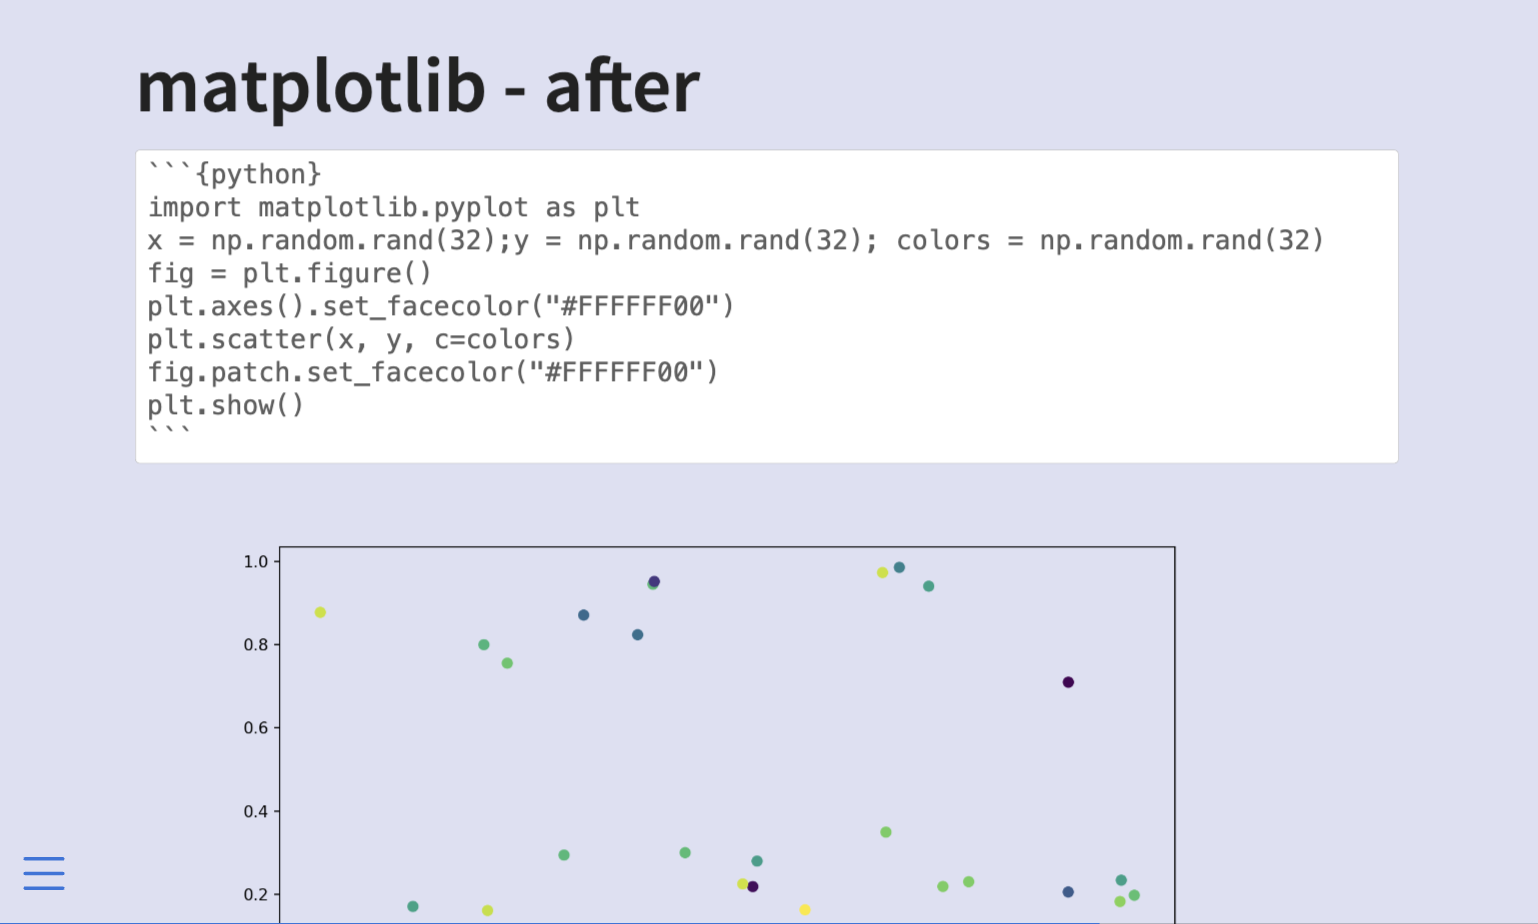
\includegraphics[keepaspectratio]{media/matplotlib-after.png}}\end{minipage}%

\end{figure}%

\subsection{seaborn}\label{seaborn}

For seaborn, we also set it twice, both of them in \texttt{set\_style()}

\begin{Shaded}
\begin{Highlighting}[]
\NormalTok{sns.set\_style(rc}\OperatorTok{=}\NormalTok{\{}\StringTok{\textquotesingle{}axes.facecolor\textquotesingle{}}\NormalTok{:}\StringTok{\textquotesingle{}\#FFFFFF00\textquotesingle{}}\NormalTok{, }
                  \StringTok{\textquotesingle{}figure.facecolor\textquotesingle{}}\NormalTok{:}\StringTok{\textquotesingle{}\#FFFFFF00\textquotesingle{}}\NormalTok{\})}
\end{Highlighting}
\end{Shaded}

\begin{figure}

\begin{minipage}{0.50\linewidth}
\pandocbounded{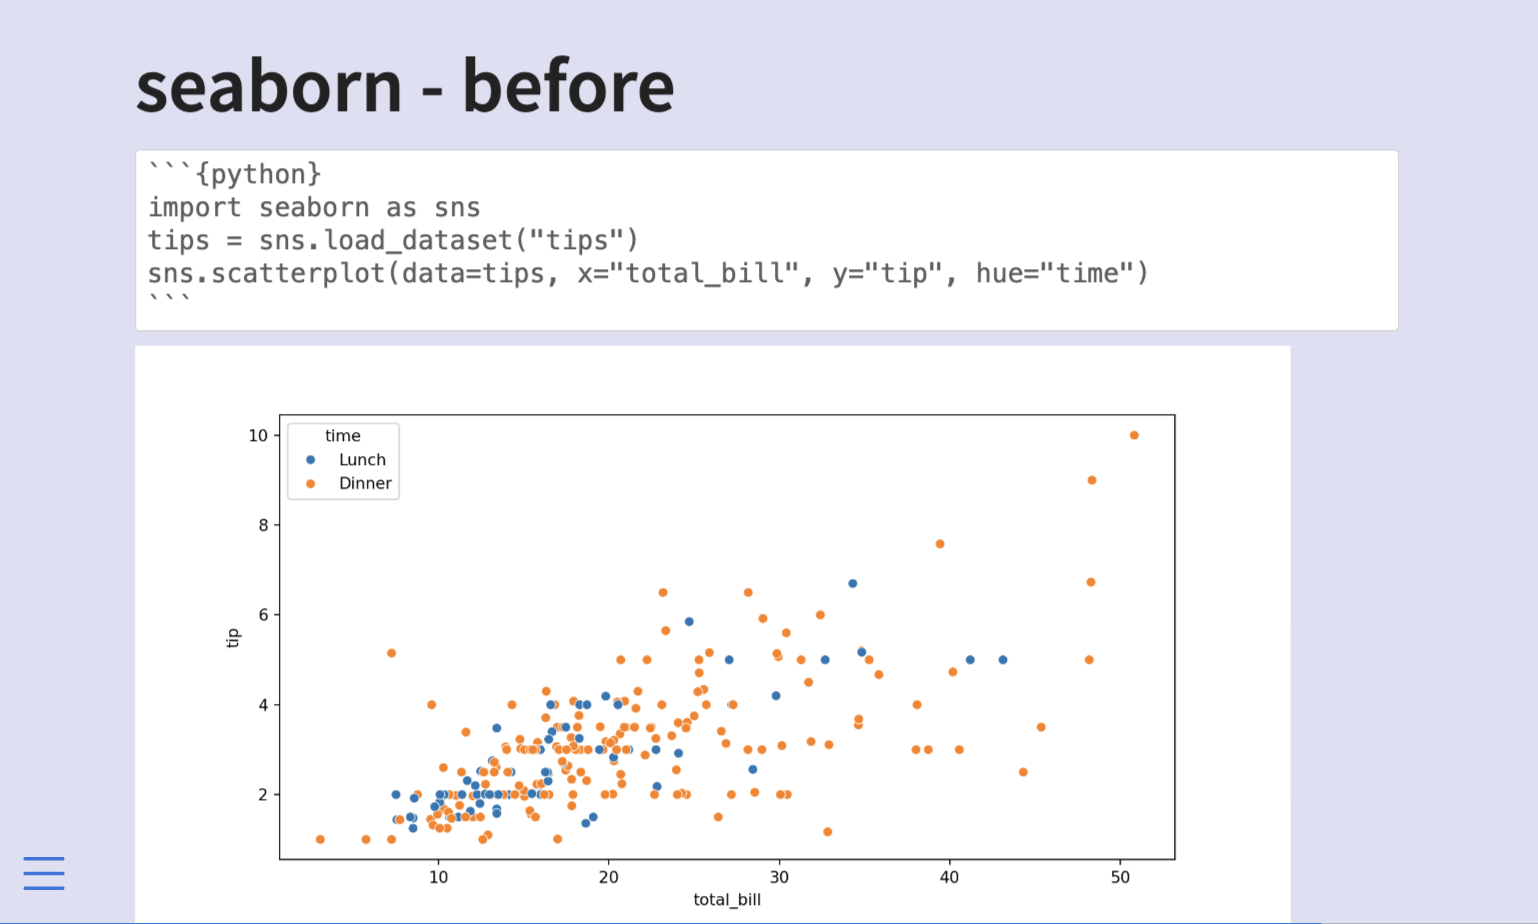
\includegraphics[keepaspectratio]{media/seaborn-before.png}}\end{minipage}%
%
\begin{minipage}{0.50\linewidth}
\pandocbounded{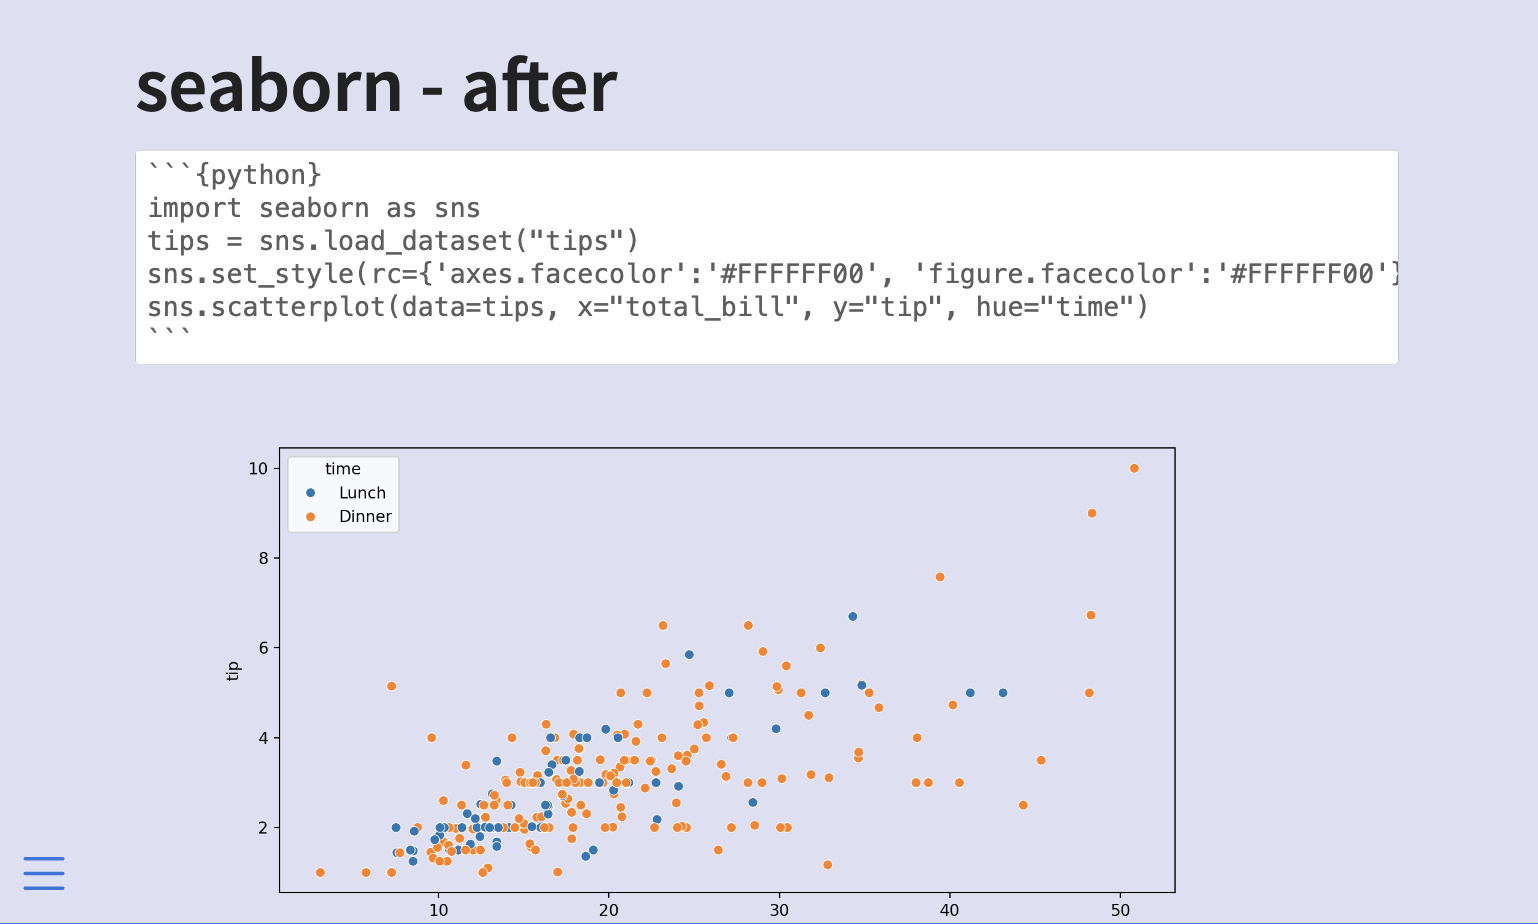
\includegraphics[keepaspectratio]{media/seaborn-after.png}}\end{minipage}%

\end{figure}%

\subsection{Source Document}\label{source-document}

The above was generated with this document.

\faIcon{file}source document

\section{Plot sizing}\label{plot-sizing}

Plots and charts are useful in slides. But we need to make sure they are
sized correctly to be as effective as possible.

\subsection{auto-stretch option}\label{auto-stretch-option}

Revealjs slides default to having the option
\href{https://quarto.org/docs/presentations/revealjs/advanced.html\#stretch}{auto-stretch:
true}, this ensures that figures always fit inside the slide. You can
turn it off globally like this.

\begin{Shaded}
\begin{Highlighting}[]
\FunctionTok{format}\KeywordTok{:}
\AttributeTok{  }\FunctionTok{revealjs}\KeywordTok{:}
\AttributeTok{    }\FunctionTok{auto{-}stretch}\KeywordTok{:}\AttributeTok{ }\CharTok{false}
\end{Highlighting}
\end{Shaded}

or on a slide-by-slide basis by adding the \texttt{.nostretch} class to
the slide.

\begin{Shaded}
\begin{Highlighting}[]
\FunctionTok{\#\# Slide Title \{.nostretch\}}
\end{Highlighting}
\end{Shaded}

We see how they affect sizing in the following slides first with the
default, and second with \texttt{.nostretch}.

\pandocbounded{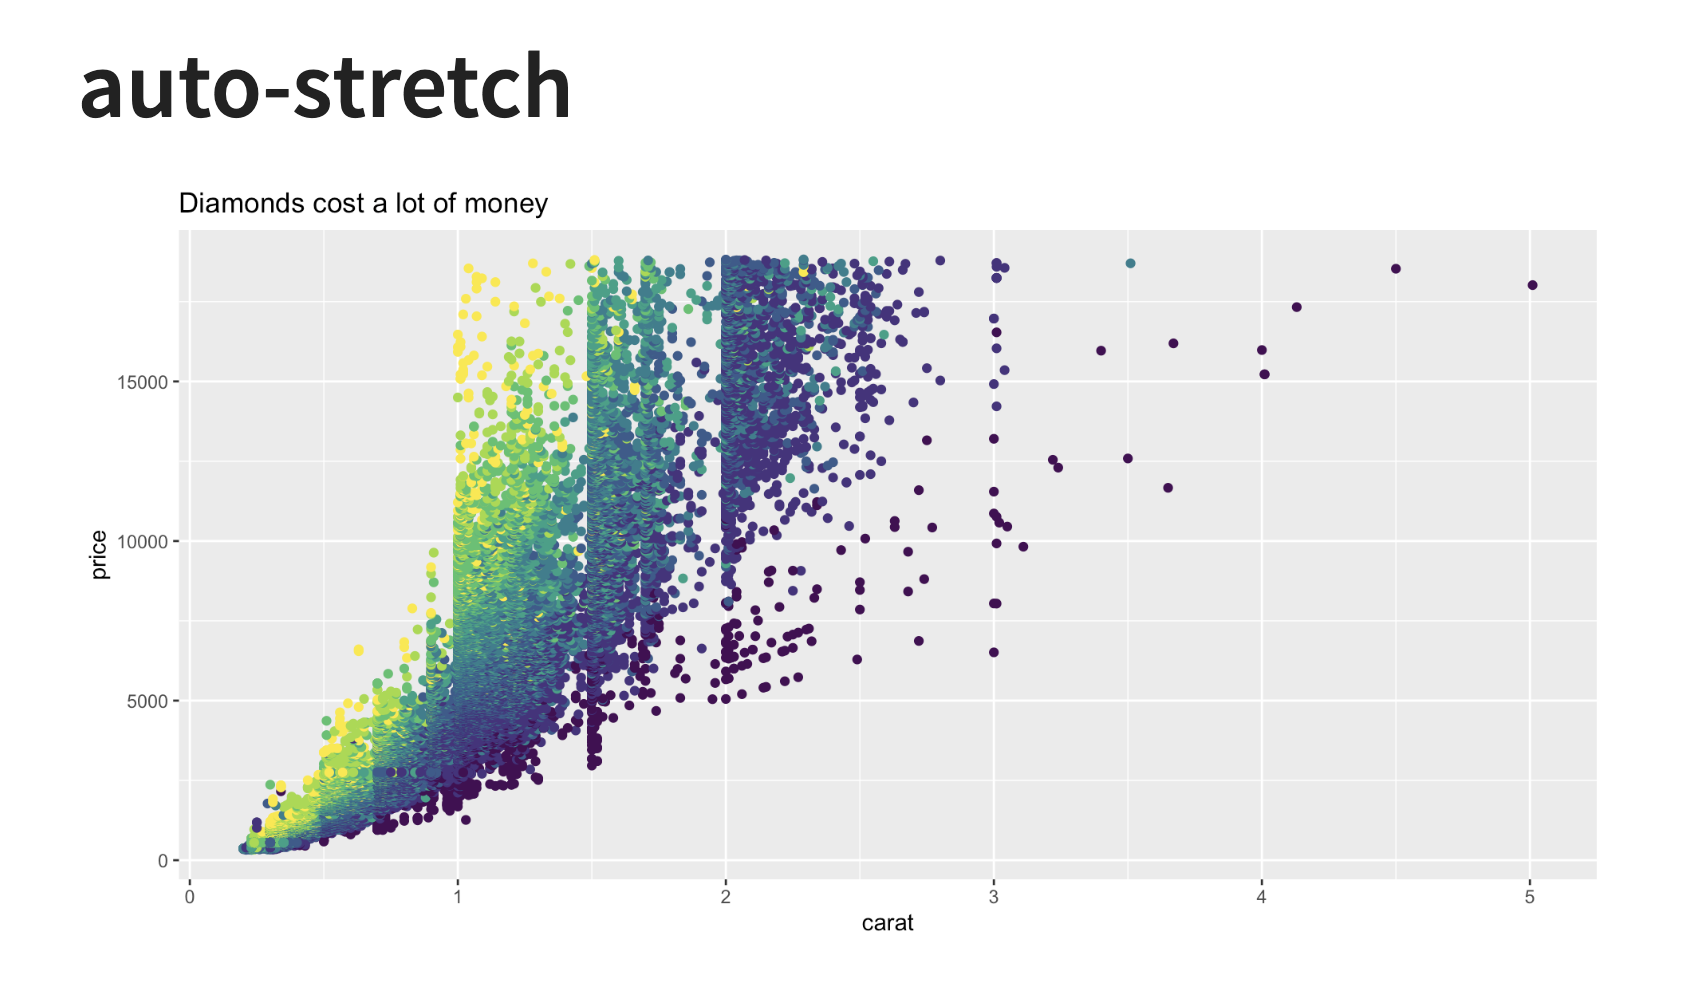
\includegraphics[keepaspectratio]{media/figures/1.png}}

\pandocbounded{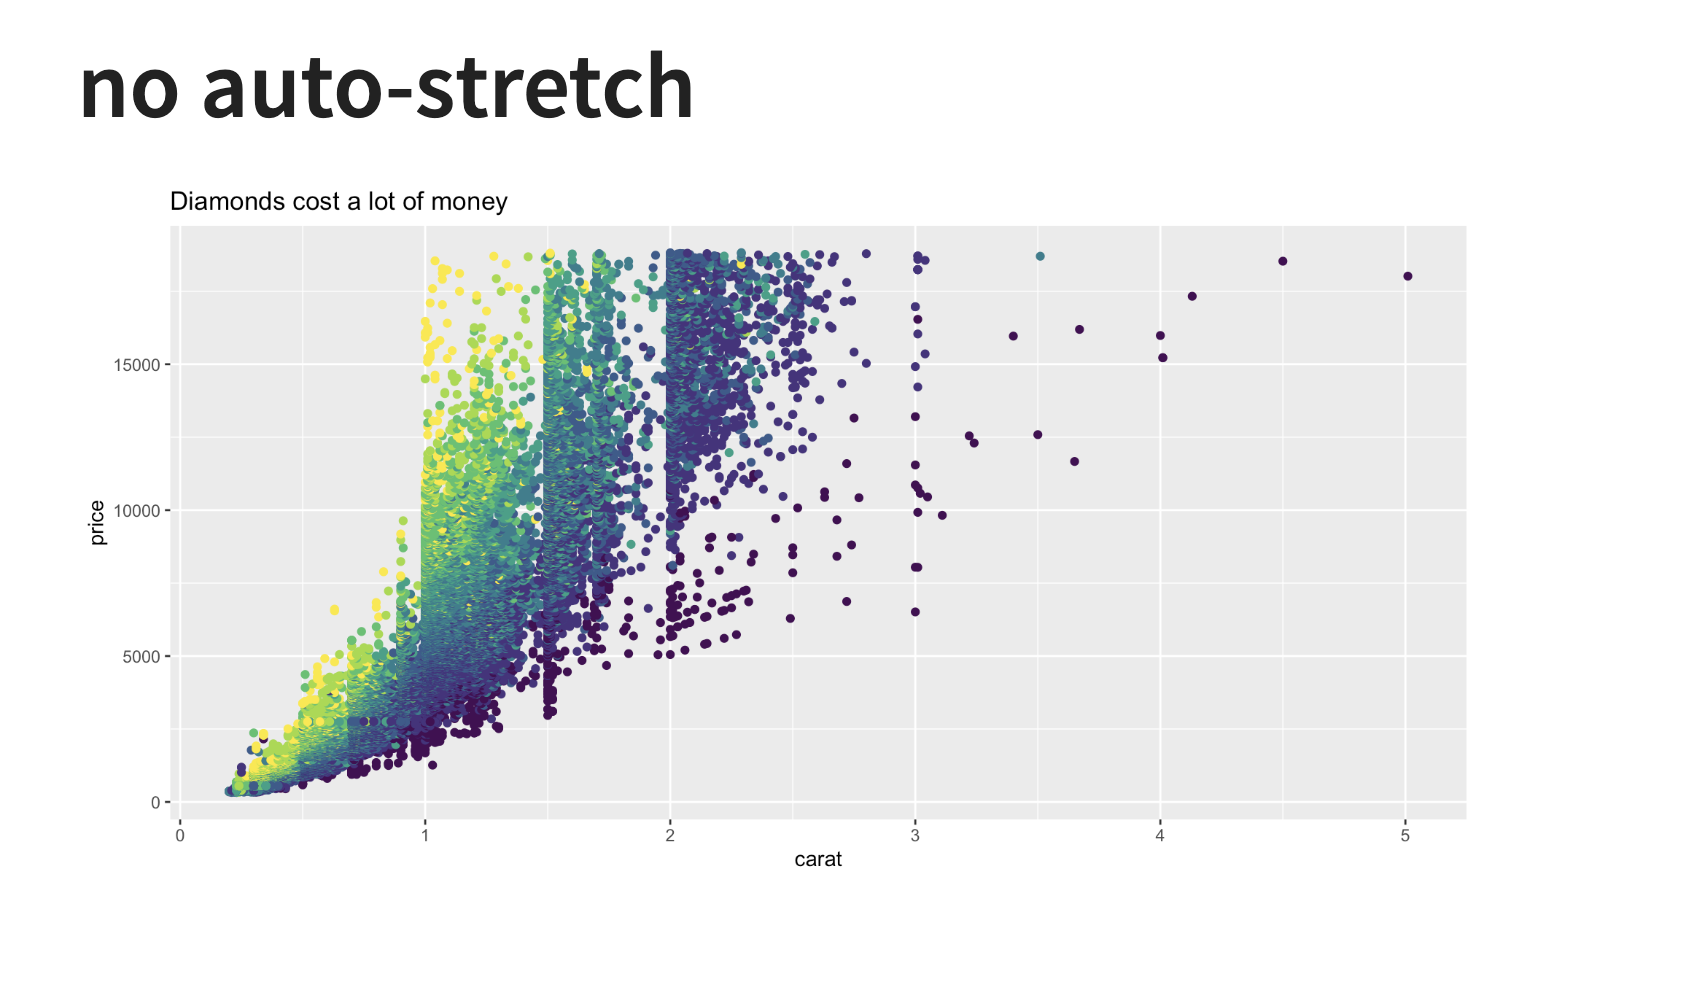
\includegraphics[keepaspectratio]{media/figures/2.png}}

By themselves, they look pretty similar. One occasion where you really
notice the difference is when there are other elements on the slide.
\texttt{auto-stretch} makes sure the image fits by making the image
smaller as seen below.

\pandocbounded{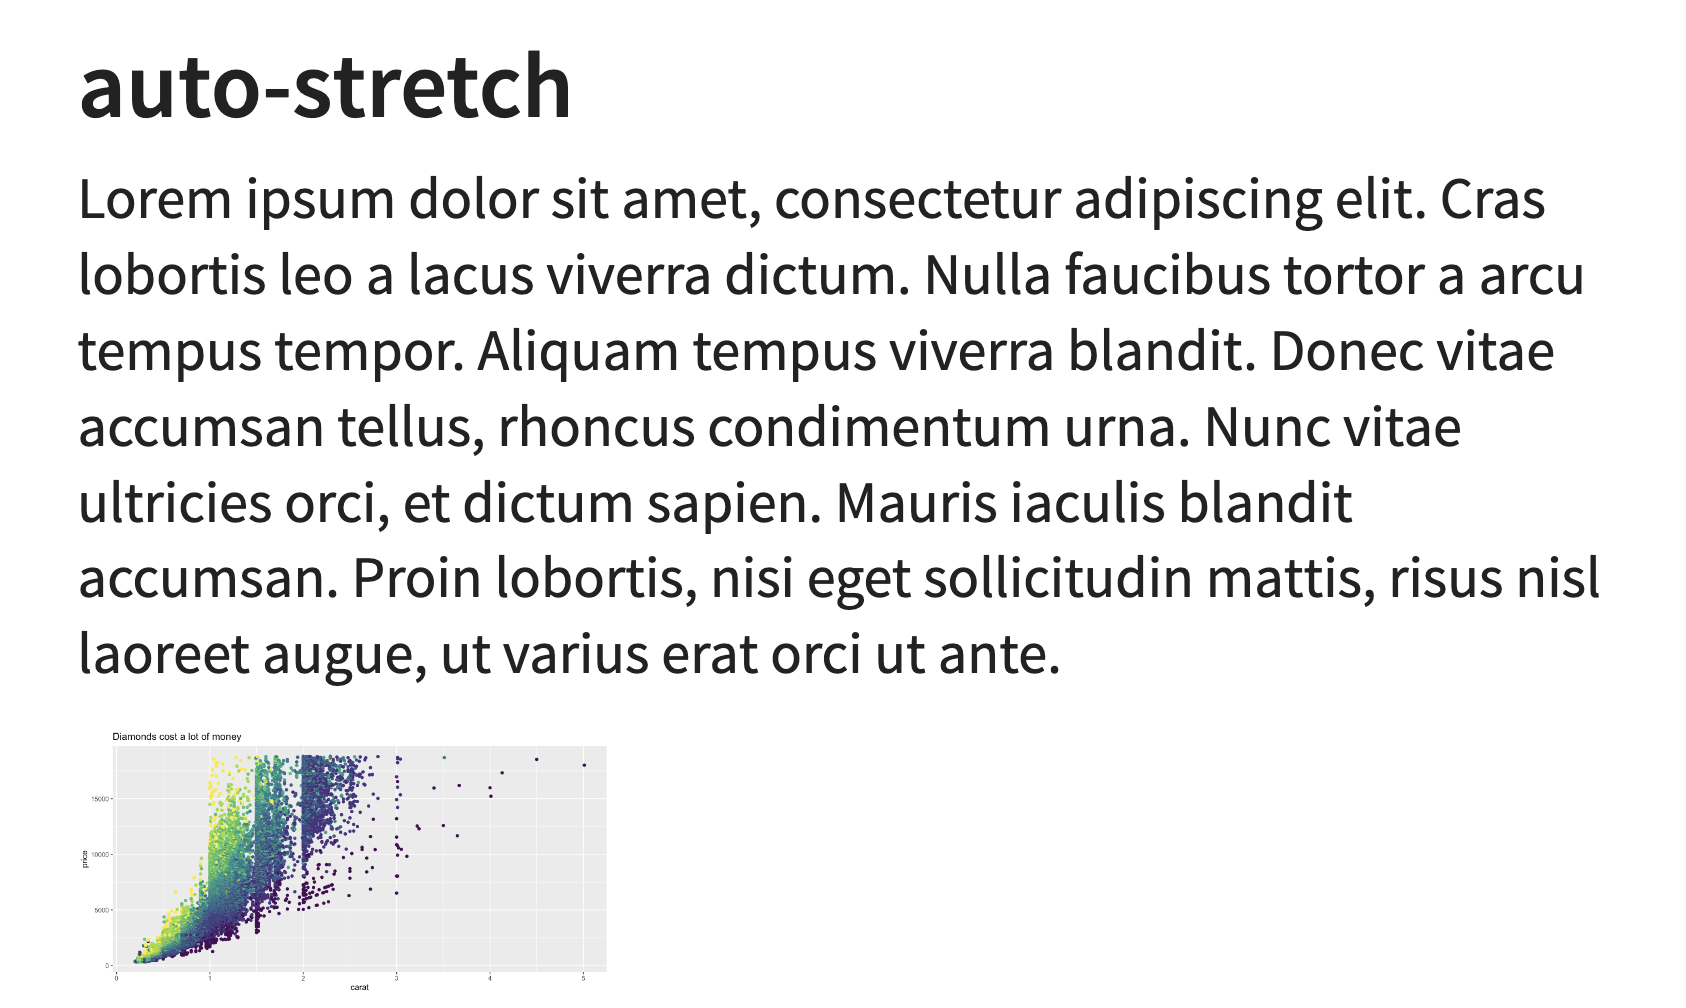
\includegraphics[keepaspectratio]{media/figures/3.png}}

\pandocbounded{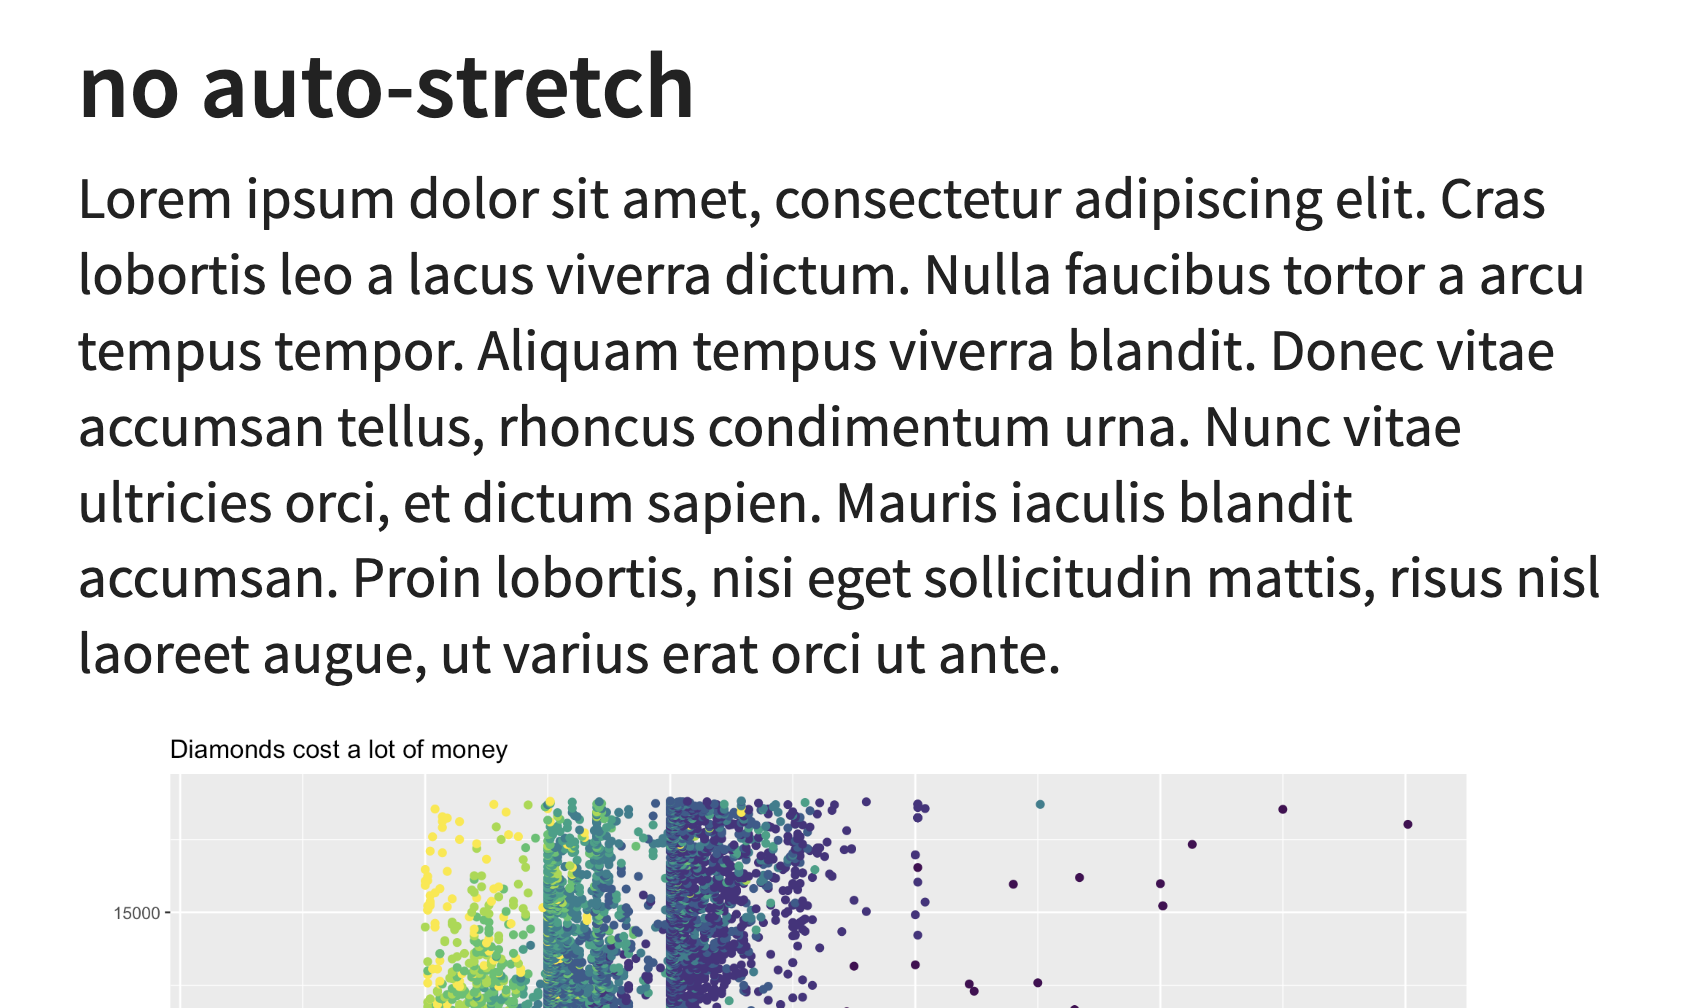
\includegraphics[keepaspectratio]{media/figures/4.png}}

\subsection{Sizing Options}\label{sizing-options}

When sizing plots we need to remember that we have to deal with two
kinds of sizes. First is the size of the actual file on disk, this is
controlled using \texttt{out-width} and \texttt{out-height}. Next is how
big the image is supposed to be in the document, which is controlled
using \texttt{fig-width}, \texttt{fig-height}, and/or \texttt{fig-asp}.
Lastly, you can control the location using \texttt{fig-align} and the
resolution using \texttt{fig-dpi}.

All of these numbers will change depending on whether you have a title
or other elements on your slides, what fonts you use, and the aspect
ratio of the slides themselves.

\subsubsection{out-width, out-height}\label{out-width-out-height}

Setting these options affects the size of the resulting image on disk.
If they are set smaller than usual, we get an image that doesn't take up
the whole screen.

\begin{Shaded}
\begin{Highlighting}[]
\InformationTok{\textasciigrave{}\textasciigrave{}\textasciigrave{}\{r\}}
\InformationTok{\#| out{-}width: 6in}
\InformationTok{\#| out{-}height: 3.5in}
\InformationTok{\textasciigrave{}\textasciigrave{}\textasciigrave{}}
\end{Highlighting}
\end{Shaded}

\pandocbounded{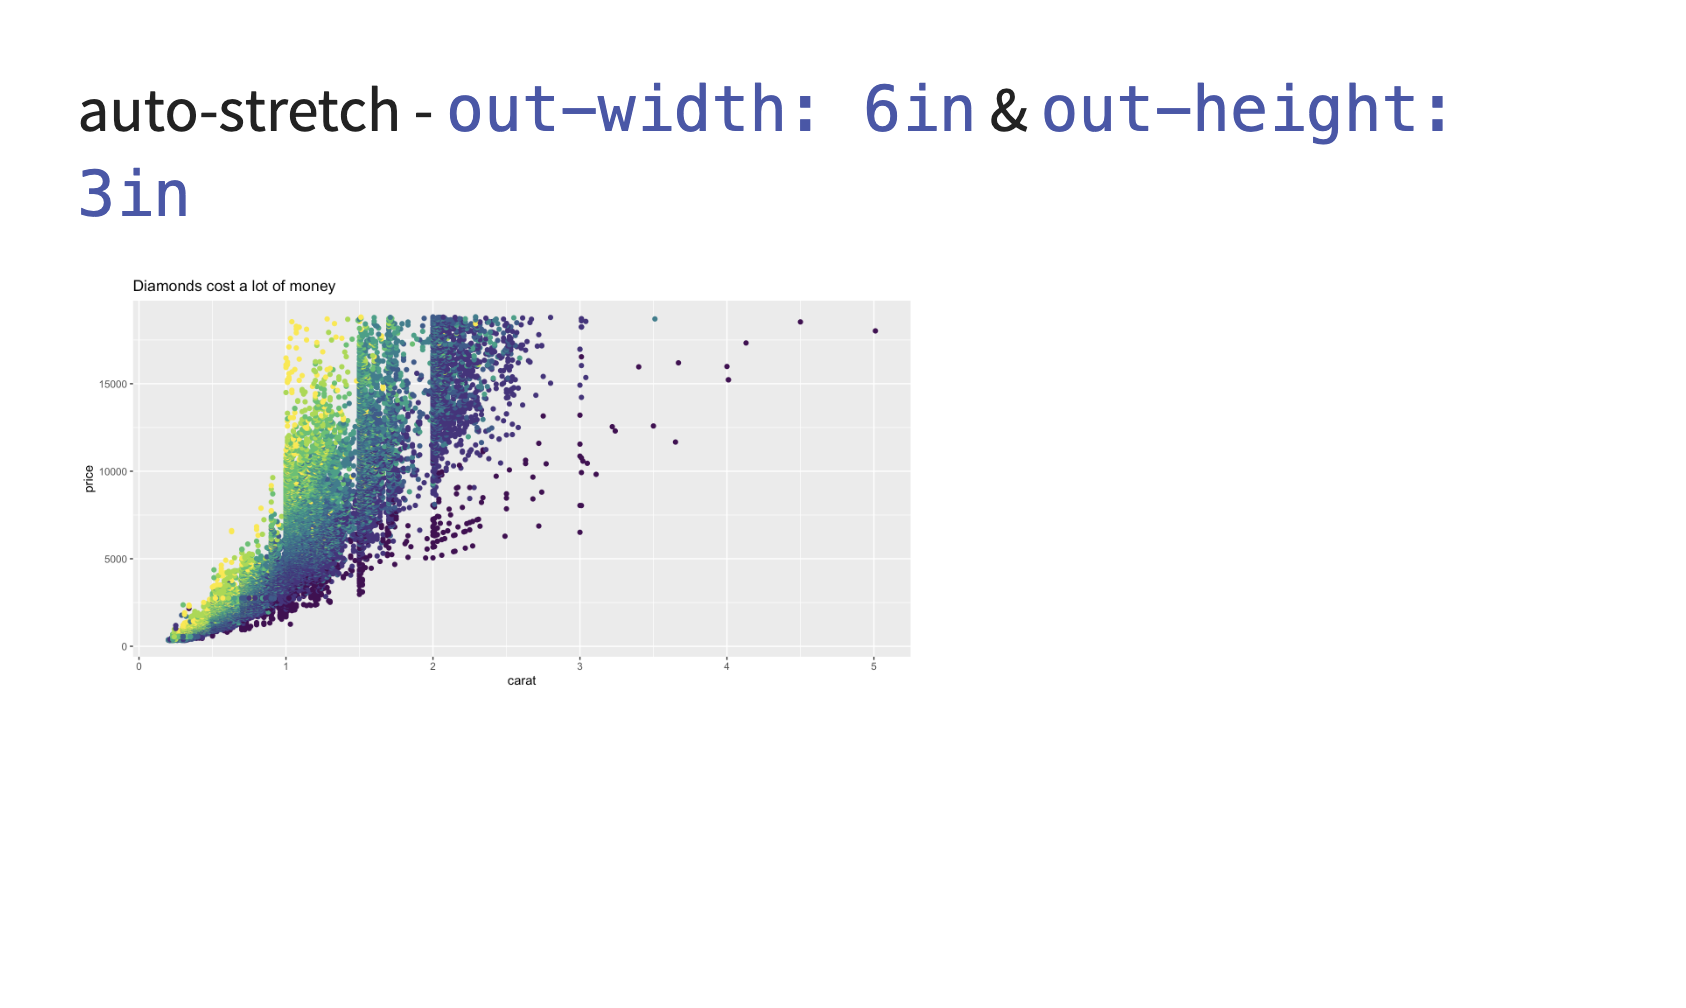
\includegraphics[keepaspectratio]{media/figures/5.png}}

\pandocbounded{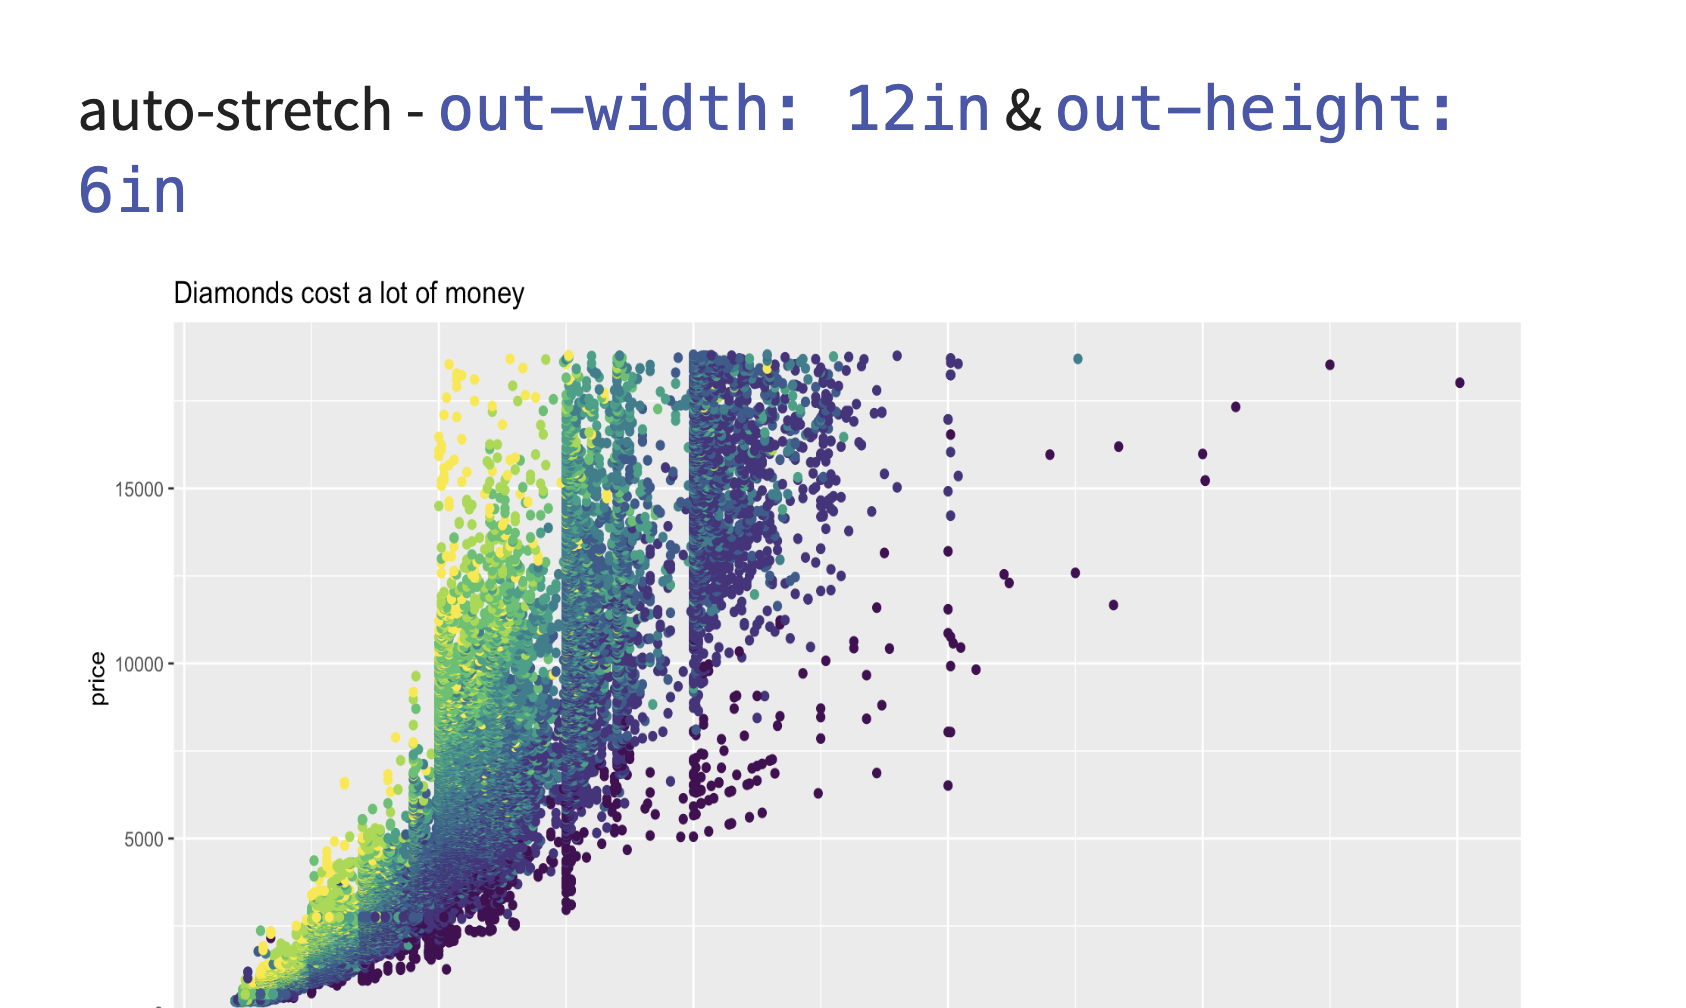
\includegraphics[keepaspectratio]{media/figures/6.png}}

I don't find myself using these options much as I tend to want images
that take up most of the space, but they are useful to know.

\subsection{fig-width, fig-height}\label{fig-width-fig-height}

I end up using \texttt{fig-width} and \texttt{fig-height} the most out
of the options shown in this blog post. I find that the default values
are too high, making the text on the plot too small for the viewer to
see. Especially for an in-person audience.

Below is the same chart 4 times with different value pairs for
\texttt{fig-width} and \texttt{fig-height}. notice how the default
values appear to be around \texttt{fig-width:\ 9} and
\texttt{fig-height:\ 5}.

\pandocbounded{\includegraphics[keepaspectratio]{media/figures/7.png}}

\pandocbounded{\includegraphics[keepaspectratio]{media/figures/8.png}}

\pandocbounded{\includegraphics[keepaspectratio]{media/figures/9.png}}

\pandocbounded{\includegraphics[keepaspectratio]{media/figures/10.png}}

All of the above figures have roughly the same aspect ratios, but if you
want others you just specify different values. Like this square chart
below.

\pandocbounded{\includegraphics[keepaspectratio]{media/figures/11.png}}

\subsection{fig-asp}\label{fig-asp}

You might have noticed that the ratios shown in the last section weren't
identical. Because unless you deal with 1-2 or 1-1 ratios you are going
to get decimals very fast. And you have to recalculate small things over
and over again. This is why \texttt{fig-asp} is amazing. Simply
determine the aspect ratio between the height and width, set that as the
\texttt{fig-asp} and then you just have to set one of
\texttt{fig-height} or \texttt{fig-width}. Is it too small? increase
\texttt{fig-height} and keep \texttt{fig-asp} the same. is it too big?
decrease \texttt{fig-height} and keep \texttt{fig-asp} the same.

\pandocbounded{\includegraphics[keepaspectratio]{media/figures/12.png}}

\pandocbounded{\includegraphics[keepaspectratio]{media/figures/13.png}}

\subsection{fig-align}\label{fig-align}

Unless your chart fits fully inside the slide then it tends to be left
aligned, you can change that with \texttt{fig-align}, setting it to
\texttt{left}, \texttt{center} or \texttt{right}.

\pandocbounded{\includegraphics[keepaspectratio]{media/figures/14.png}}

\pandocbounded{\includegraphics[keepaspectratio]{media/figures/15.png}}

\pandocbounded{\includegraphics[keepaspectratio]{media/figures/16.png}}

\subsection{fig-dpi}\label{fig-dpi}

Lastly, something you might need to worry about is the \textbf{D}ots
\textbf{P}er \textbf{I}nch (DPI) specified by \texttt{fig-dpi}. This is
a measure of resolution in your chart. If you see your chart becoming a
little blurry, increase the dpi until it isn't anymore. Note that dpi
will result in larger file sizes, so only change if you have to.

\pandocbounded{\includegraphics[keepaspectratio]{media/figures/17.png}}

\pandocbounded{\includegraphics[keepaspectratio]{media/figures/18.png}}

\subsection{Make work with columns}\label{make-work-with-columns}

even if you set the option globally, you will have to make
slide-by-slide adjustments, such as with charts in \texttt{.columns}.
Below is one example of how we can modify the \texttt{fig-asp} to make
it look decent in a column layout.

\pandocbounded{\includegraphics[keepaspectratio]{media/figures/19.png}}

\subsection{Source Document}\label{source-document-1}

The above was generated with this document.

\faIcon{file}source document

\chapter{Layout}\label{layout}

\section{Pulling things left and
right}\label{pulling-things-left-and-right}

Using
\href{https://quarto.org/docs/presentations/revealjs/\#multiple-columns}{multiple
columns} is a nice way to split up the content of your slides. I use it
so much that I have a
\href{https://rstudio.github.io/rstudio-extensions/rstudio_snippets.html}{snippet}
to save time since I use it so much. It works great for side-by-side
comparisons as well. This is done using the following syntax. We use the
\texttt{width} attribute to determine the width of each of the columns.

\begin{Shaded}
\begin{Highlighting}[]
\NormalTok{:::: \{.columns\}}

\NormalTok{::: \{.column width="40\%"\}}
\NormalTok{Left column}
\NormalTok{:::}

\NormalTok{::: \{.column width="60\%"\}}
\NormalTok{Right column}
\NormalTok{:::}

\NormalTok{::::}
\end{Highlighting}
\end{Shaded}

but you can use it in quite a few ways beyond this! Firstly, each column
is by itself a div, so you can style it directly. Such as making the
right column have the right aligned text.

\begin{Shaded}
\begin{Highlighting}[]
\NormalTok{:::: \{.columns\}}

\NormalTok{::: \{.column width="50\%"\}}
\NormalTok{Left column}
\NormalTok{:::}

\NormalTok{::: \{.column width="50\%" style="text{-}align: right;"\}}
\NormalTok{Right column}
\NormalTok{:::}

\NormalTok{::::}
\end{Highlighting}
\end{Shaded}

The structure of columns doesn't require that we just use 2 columns. You
can do as many columns as you want, but generally, you will have a hard
time using more than 4.

\begin{Shaded}
\begin{Highlighting}[]
\NormalTok{:::: \{.columns\}}

\NormalTok{::: \{.column width="25\%"\}}
\NormalTok{1st column}
\NormalTok{:::}

\NormalTok{::: \{.column width="25\%"\}}
\NormalTok{2nd column}
\NormalTok{:::}

\NormalTok{::: \{.column width="25\%"\}}
\NormalTok{3rd column}
\NormalTok{:::}

\NormalTok{::: \{.column width="25\%"\}}
\NormalTok{4th column}
\NormalTok{:::}

\NormalTok{::::}
\end{Highlighting}
\end{Shaded}

Another way I like to use columns is by keeping one of them empty. This
way provides a fast and easy way to add space or put text in specific
locations.

\begin{Shaded}
\begin{Highlighting}[]
\NormalTok{:::: \{.columns\}}

\NormalTok{::: \{.column width="30\%"\}}
\NormalTok{:::}

\NormalTok{::: \{.column width="70\%"\}}
\NormalTok{Only right side}
\NormalTok{:::}

\NormalTok{::::}
\end{Highlighting}
\end{Shaded}

\faIcon{file}qmd

\section{r-fit-text}\label{r-fit-text}

Another quick way to change the layout of your slide is to let the text
take up the entire slide real estate. We can do this using the
\href{https://quarto.org/docs/presentations/revealjs/advanced.html\#fit-text}{r-fit-text}
class using the following syntax. This will make the text so big that it
takes up all the horizontal space on the slide.

\begin{Shaded}
\begin{Highlighting}[]
\NormalTok{::: r{-}fit{-}text}
\NormalTok{Big Text}
\NormalTok{:::}
\end{Highlighting}
\end{Shaded}

This works well combined with the
\href{https://quarto.org/docs/presentations/revealjs/advanced.html\#center}{center}
class, which makes sure the text appears in the center vertically on the
slide.

\begin{Shaded}
\begin{Highlighting}[]
\FunctionTok{\#\# \{.center\}}

\NormalTok{::: r{-}fit{-}text}
\NormalTok{This fits perfectly!}
\NormalTok{:::}
\end{Highlighting}
\end{Shaded}

One thing about using \texttt{r-fit-text} is that it applies the same
text size to all the text inside it, so when you use it across multiple
lines, you won't get the same effect.

\begin{Shaded}
\begin{Highlighting}[]
\NormalTok{::: r{-}fit{-}text}
\NormalTok{This fits perfectly!}

\NormalTok{On two lines}
\NormalTok{:::}
\end{Highlighting}
\end{Shaded}

This can however be fixed, by using a \texttt{r-fit-text} for each line
of text.

\begin{Shaded}
\begin{Highlighting}[]
\NormalTok{::: r{-}fit{-}text}
\NormalTok{This fits perfectly!}
\NormalTok{:::}

\NormalTok{::: r{-}fit{-}text}
\NormalTok{On two lines}
\NormalTok{:::}
\end{Highlighting}
\end{Shaded}

\faIcon{file}qmd

\section{Using images}\label{using-images}

Using images for style is another thing you can do to change the layout.
If you don't have much content on your slides. e.i. just a sentence or
two. You could pair that with an image that relays some of the same
information. These images will typically not contain content themselves
but rather reinforce the content on the slides.

There are 3 main ways to include images. Using the
\href{https://quarto.org/docs/authoring/figures.html}{basics}, using
\href{https://quarto.org/docs/presentations/revealjs/advanced.html\#absolute-position}{absolute
position} or as
\href{https://quarto.org/docs/presentations/revealjs/\#image-backgrounds}{background
images}.

\subsection{Basic figures}\label{basic-figures}

The basic way of adding figures is using the following syntax

\begin{Shaded}
\begin{Highlighting}[]
\AlertTok{![](holly{-}mandarich.jpg)}
\end{Highlighting}
\end{Shaded}

where \texttt{holly-mandarich.jpg} is the path to the image. We can
change some options such as adding \texttt{\{fig-align="right"\}} to the
end to change the alignment. But I end up not using this style that much
because it is added as content, so it will push other content around,
and it adheres to margins which I rarely want for tasks like this.

Photo by Holly Mandarich on Unsplash

\faIcon{file}qmd

\subsection{Absolute position}\label{absolute-position}

Absolute is my favorite way of adding images. It gives me much more
control over where the image is located and its size.

You use the following syntax:

\begin{Shaded}
\begin{Highlighting}[]
\AlertTok{![](noelle{-}rebekah.jpg)}\NormalTok{\{.absolute top=0 right=0 height="100\%"\}}
\end{Highlighting}
\end{Shaded}

Where you can use the following attributes:

\begin{longtable}[]{@{}ll@{}}
\toprule\noalign{}
Attribute & Description \\
\midrule\noalign{}
\endhead
\bottomrule\noalign{}
\endlastfoot
\texttt{width} & Width of element \\
\texttt{height} & Height of element \\
\texttt{top} & Distance from top of slide \\
\texttt{left} & Distance from left of slide \\
\texttt{bottom} & Distance from bottom of slide \\
\texttt{right} & Distance from right of slide \\
\end{longtable}

you need one of \texttt{left} and \texttt{right} and one of
\texttt{bottom} and \texttt{top} to give the correct location. I find
that just using one of \texttt{width} or \texttt{height} is easier as it
doesn't distort the image. All of these attributes accept all known CSS
values, such as pixels, inches, and percentages.
\href{https://developer.mozilla.org/en-US/docs/Web/CSS/length}{All about
CSS length} for more information.

All images in revealjs default to the following maximum sizes:

\begin{Shaded}
\begin{Highlighting}[]
\NormalTok{max{-}width}\InformationTok{:}\NormalTok{ 95\%;}
\NormalTok{max{-}height}\InformationTok{:}\NormalTok{ 95\%;}
\end{Highlighting}
\end{Shaded}

No matter how large we set \texttt{width} or \texttt{height} we are
overruled by \texttt{max-width} and \texttt{max-height}. We can make the
image any size by overruling those. Specifically, we can unset them with
\texttt{style="max-height:\ unset;\ max-width:\ unset;"}.

With some experimentation, we can size the image such that it is where
we want it. Notice that we are using negative locations to make this
happen as \texttt{0} is inside the slide.

\begin{Shaded}
\begin{Highlighting}[]
\AlertTok{![](noelle{-}rebekah.jpg)}\NormalTok{\{.absolute top="{-}10\%" right="{-}10\%" height="120\%" style="max{-}height: unset;"\}}
\end{Highlighting}
\end{Shaded}

Photo by Noelle Rebekah on Unsplash

\faIcon{file}qmd

\begin{tcolorbox}[enhanced jigsaw, titlerule=0mm, bottomrule=.15mm, opacityback=0, colbacktitle=quarto-callout-warning-color!10!white, colframe=quarto-callout-warning-color-frame, coltitle=black, breakable, toprule=.15mm, colback=white, bottomtitle=1mm, title=\textcolor{quarto-callout-warning-color}{\faExclamationTriangle}\hspace{0.5em}{Warning}, toptitle=1mm, arc=.35mm, left=2mm, leftrule=.75mm, rightrule=.15mm, opacitybacktitle=0.6]

Since the way that positions are done in revealjs, it can be almost
impossible to have the above effect for all aspect ratios. Make it work
for the aspect ratio you use, and have peace.

\end{tcolorbox}

\section{Absolute position
everything}\label{absolute-position-everything}

It took me too long to realize, but the
\href{https://quarto.org/docs/presentations/revealjs/advanced.html\#absolute-position}{absolute}
class can be used on anything!

You might have seen the following syntax to place an image anywhere

\begin{Shaded}
\begin{Highlighting}[]
\AlertTok{![](image1.png)}\NormalTok{\{.absolute top=200 left=0 width="350" height="300"\}}
\end{Highlighting}
\end{Shaded}

But you are not restricted in using it with images. The following
results in the image you see attached:

I like to use it with text in the following way:

\begin{Shaded}
\begin{Highlighting}[]
\CommentTok{[}\OtherTok{python is great}\CommentTok{]}\NormalTok{\{.absolute bottom="45\%" left="20\%"\}}

\CommentTok{[}\OtherTok{and so is R}\CommentTok{]}\NormalTok{\{.absolute bottom="0\%" right="0\%"\}}
\end{Highlighting}
\end{Shaded}

\faIcon{file}qmd

\subsection{Background image}\label{background-image}

The last way to add images, which I highly recommend is the use of
background images. And in many ways, it is the simplest one.

you specify it on the slide level in the following way:

\begin{Shaded}
\begin{Highlighting}[]
\FunctionTok{\#\# Slide Title \{background{-}image="galen{-}crout.jpg"\}}
\end{Highlighting}
\end{Shaded}

you can set other options such as
\href{https://developer.mozilla.org/docs/Web/CSS/background-position}{background-position}
and
\href{https://developer.mozilla.org/docs/Web/CSS/background-repeat}{background-repeat}
but I rarely end up using them.

I end up not setting a default title and use \texttt{.absolute} to place
any content I want where I want it.

\begin{Shaded}
\begin{Highlighting}[]
\FunctionTok{\#\# \{background{-}image="galen{-}crout.jpg"\}}

\CommentTok{[}\OtherTok{always explore}\CommentTok{]}\NormalTok{\{.absolute left="50\%" top="20\%" style="rotate: {-}10deg;"\}}
\end{Highlighting}
\end{Shaded}

Photo by Galen Crout on Unsplash

\faIcon{file}qmd

As we see here, the text positioning can change how the slides are
perceived. Both in style and emotion, try to think about how you can
incorporate text positioning to maximize engagement.

\section{Overlayed Text Boxes}\label{overlayed-text-boxes}

When using background images, it can be hard to place text on top of it,
in a way that that keeps the text readable. This is often an issue with
images that are more busy or have colors that match. A simple fix is to
overlay a box, and we then add text on you. If we take the first slide
here as an example.

\begin{Shaded}
\begin{Highlighting}[]
\FunctionTok{\#\# \{background{-}image="tim{-}marshall.jpg"\}}
\end{Highlighting}
\end{Shaded}

First, we try to use \texttt{.absolute} to add some inspiring text. It
adds text, but it is not easy to read at all!!

\begin{Shaded}
\begin{Highlighting}[]
\FunctionTok{\#\# \{background{-}image="tim{-}marshall.jpg"\}}

\NormalTok{::: \{.absolute left="55\%" top="55\%" style="font{-}size:1.8em;"\}}
\NormalTok{Be Brave}

\NormalTok{Take Risks}
\NormalTok{:::}
\end{Highlighting}
\end{Shaded}

But we can expand on this idea, adding a \texttt{background-color} to
make it stand out. We also added some \texttt{padding}, otherwise the
background would just be slightly bigger than the text itself.

\section{}\label{section}

\begin{Shaded}
\begin{Highlighting}[]
\NormalTok{::: \{.absolute left="55\%" top="55\%" style="font{-}size:1.8em; padding: 0.5em 1em; background{-}color: rgba(255, 255, 255, .5);"\}}
\NormalTok{Be Brave}

\NormalTok{Take Risks}
\NormalTok{:::}
\end{Highlighting}
\end{Shaded}

it already looks quite good! We can make it pop just a little bit more,
by adding a \texttt{backdrop-filter} to make it look a little
glass-like, adding a \texttt{box-shadow} to make it look a little
3-dimensional, and adding a small \texttt{border-radius} to stop the
sharp corners.

\begin{Shaded}
\begin{Highlighting}[]
\FunctionTok{\#\# \{background{-}image="tim{-}marshall.jpg"\}}

\NormalTok{::: \{.absolute left="55\%" top="55\%" style="font{-}size:1.8em; padding: 0.5em 1em; background{-}color: rgba(255, 255, 255, .5); backdrop{-}filter: blur(5px); box{-}shadow: 0 0 1rem 0 rgba(0, 0, 0, .5); border{-}radius: 5px;"\}}
\NormalTok{Be Brave}

\NormalTok{Take Risks}
\NormalTok{:::}
\end{Highlighting}
\end{Shaded}

Photo by Tim Marshall on Unsplash

\faIcon{file}qmd

I think this turned out well. There are endless ways to use this. It is
quite CSS-heavy work, but I think it is worth it. Note that you are
always free to copy an example and modify it to your wants.

\section{Vary the type of slides}\label{vary-the-type-of-slides}

This post has shown a number of ways to place content on your slides. My
final advice in this post is to use some of these tips to vary how the
content is laid out. It doesn't have to be over the top, but slight
variations can help a slide deck feel fresh.

\chapter{Manual code}\label{manual-code}

\section{Hand-styled code chunks}\label{hand-styled-code-chunks}

With a little extra effort, you can create highlighted code chunks. This
is different than the code highlighting that comes naturally. In this
instance, we are creating an unstyled code chunk, and styling part of
the code manually with css classes.

First, we write a new css class, I like to call it \texttt{.mono}. The
important thing is that we set \texttt{font-family:\ monospace;}, but we
can do other things, like setting the \texttt{font-size}.

\begin{Shaded}
\begin{Highlighting}[]
\FunctionTok{.mono}\NormalTok{ \{}
  \KeywordTok{font{-}family}\NormalTok{: }\DecValTok{monospace}\OperatorTok{;}
  \KeywordTok{font{-}size}\NormalTok{: }\DecValTok{0.9}\DataTypeTok{em}\OperatorTok{;}
\NormalTok{\}}
\end{Highlighting}
\end{Shaded}

Next, we add our code in a fenced div, with the mono class. you need to
use \texttt{\textbackslash{}} to add leading spaces, and each line ends
with 2 spaces to denote newlines

\begin{Shaded}
\begin{Highlighting}[]
\NormalTok{::: mono}
\NormalTok{library(ggplot2)}
\NormalTok{mtcars |\textgreater{}  }
\NormalTok{\textbackslash{} \textbackslash{} ggplot(aes(mpg, disp)) +  }
\NormalTok{\textbackslash{} \textbackslash{} geom\_point() +  }
\NormalTok{\textbackslash{} \textbackslash{} geom\_smooth(method = "lm", formula = "y \textasciitilde{} x")}
\NormalTok{:::}
\end{Highlighting}
\end{Shaded}

Taking it to the next step, you can manually change the formatting of
functions using css or css classes,
\texttt{library({[}ggplot2{]}\{style="color:purple;"\})} would make
\texttt{ggplot2} purple. This is also a great place to use
\href{https://emilhvitfeldt.com/post/slidecraft-colors-fonts/\#using-css-classes}{css
classes}.

We can take it a step further and use
\href{https://quarto.org/docs/presentations/revealjs/advanced.html\#fragments}{fragments}
to have the code highlighted one bit at a time. Changing the last line
to the following

\begin{Shaded}
\begin{Highlighting}[]
\NormalTok{geom\_smooth(}\CommentTok{[}\OtherTok{method = "lm"}\CommentTok{]}\NormalTok{\{.fragment .highlight{-}red\}, }\CommentTok{[}\OtherTok{formula = "y \textasciitilde{} x"}\CommentTok{]}\NormalTok{\{.fragment .highlight{-}blue\})}
\end{Highlighting}
\end{Shaded}

seperately highlights the code \texttt{method\ =\ "lm"} then
\texttt{formula\ =\ "y\ \textasciitilde{}\ x"} in red and blue.

\faIcon{file}qmd

\chapter{asciicast}\label{asciicast}

This chapter celebrates the
\href{https://github.com/r-lib/asciicast}{asciicast} R package to
showcase rich output.

\section{Without asciicast}\label{without-asciicast}

When R code produces messages with colors or styling, they are typically
lost when we write slides

\faIcon{file}qmd

\section{Default asciicast}\label{default-asciicast}

This is where the amazing
\href{https://github.com/r-lib/asciicast}{asciicast} R package comes
into play. \{asciicast\} takes an R script and turns it into an
\href{https://asciinema.org/}{asciinema} cast. We will use the very
convenient
\href{https://asciicast.r-lib.org/reference/init_knitr_engine.html}{init\_knitr\_engine()}
function to make this as easy as possible.

We can add the \{asciicast\} \{knitr\} engine by placing the following
chunk at the beginning of our document.

\begin{Shaded}
\begin{Highlighting}[]
\InformationTok{\textasciigrave{}\textasciigrave{}\textasciigrave{}\{r\}}
\InformationTok{asciicast::init\_knitr\_engine()}
\InformationTok{\textasciigrave{}\textasciigrave{}\textasciigrave{}}
\end{Highlighting}
\end{Shaded}

And then we toggle asciicast output by replacing

\begin{Shaded}
\begin{Highlighting}[]
\InformationTok{\textasciigrave{}\textasciigrave{}\textasciigrave{}\{r\}}
\InformationTok{library(tidymodels)}
\InformationTok{\textasciigrave{}\textasciigrave{}\textasciigrave{}}
\end{Highlighting}
\end{Shaded}

with

\begin{Shaded}
\begin{Highlighting}[]
\InformationTok{\textasciigrave{}\textasciigrave{}\textasciigrave{}\{asciicast\}}
\InformationTok{library(tidymodels)}
\InformationTok{\textasciigrave{}\textasciigrave{}\textasciigrave{}}
\end{Highlighting}
\end{Shaded}

With this change, we get the following output, nicely styled with colors
and everything.

\faIcon{file}qmd

\begin{tcolorbox}[enhanced jigsaw, titlerule=0mm, bottomrule=.15mm, opacityback=0, colbacktitle=quarto-callout-note-color!10!white, colframe=quarto-callout-note-color-frame, coltitle=black, breakable, toprule=.15mm, colback=white, bottomtitle=1mm, title=\textcolor{quarto-callout-note-color}{\faInfo}\hspace{0.5em}{Note}, toptitle=1mm, arc=.35mm, left=2mm, leftrule=.75mm, rightrule=.15mm, opacitybacktitle=0.6]

The output of asciicast will by default fill the screen horizontally,
but for some reason when setting
\texttt{format:\ revealjs:\ self-contained:\ true} it doesn't. All
examples use this option for a better blogging experience. You just have
to trust me that it looks better without the option.

\end{tcolorbox}

\section{Using startup to seed, load some
packages}\label{using-startup-to-seed-load-some-packages}

The full list of arguments to \texttt{asciicast\_init\_knitr\_engine()}
is as follows

\begin{Shaded}
\begin{Highlighting}[]
\FunctionTok{formals}\NormalTok{(asciicast}\SpecialCharTok{::}\NormalTok{init\_knitr\_engine)}
\end{Highlighting}
\end{Shaded}

\begin{verbatim}
$echo
[1] FALSE

$same_process
[1] TRUE

$timeout
[1] 10

$startup
NULL

$record_env
NULL

$echo_input
[1] TRUE

$interactive
[1] TRUE
\end{verbatim}

I will talk about the 3 I use, which are \texttt{same\_process},
\texttt{echo}, and \texttt{echo\_input}. The two go together.
\texttt{same\_process} which defaults to \texttt{TRUE}, does what it
says. It determines whether all the asciicast chunks should be in the
same process or not. If you want to show things that only happen once a
session, you might want to turn this off which is done this way

\begin{Shaded}
\begin{Highlighting}[]
\InformationTok{\textasciigrave{}\textasciigrave{}\textasciigrave{}\{r\}}
\InformationTok{asciicast::init\_knitr\_engine(}
\InformationTok{  same\_process = FALSE}
\InformationTok{)}
\InformationTok{\textasciigrave{}\textasciigrave{}\textasciigrave{}}
\end{Highlighting}
\end{Shaded}

and gives the following results

\faIcon{file}qmd

You will notice that the code that is being run is included in the
asciicast output. This is happening because the default arguments
\texttt{echo\ =\ FALSE} and \texttt{echo\_input\ =\ TRUE}. By swapping
these options we get the code as normal quarto code, with the output as
asciicast

\begin{Shaded}
\begin{Highlighting}[]
\InformationTok{\textasciigrave{}\textasciigrave{}\textasciigrave{}\{r\}}
\InformationTok{asciicast::init\_knitr\_engine(}
\InformationTok{  echo = TRUE,}
\InformationTok{  echo\_input = FALSE}
\InformationTok{)}
\InformationTok{\textasciigrave{}\textasciigrave{}\textasciigrave{}}
\end{Highlighting}
\end{Shaded}

\faIcon{file}qmd

It wouldn't make much sense to set both of these to \texttt{TRUE} as you
would have duplication, but there are certainly cases where you want
both of these to be \texttt{FALSE} as you just want the output.

\section{Using theme argument}\label{using-theme-argument}

The output is styled a certain way, and we can change it. At the time of
writing, the following 10 premade themes are available.

\begin{itemize}
\tightlist
\item
  asciinema
\item
  tango
\item
  solarized-dark
\item
  solarized-light
\item
  seti
\item
  monokai
\item
  github-light
\item
  github-dark
\item
  pkgdown
\item
  readme
\end{itemize}

We can toggle any of these by setting the option
\texttt{asciicast\_theme}. The below example showcases the
\texttt{"solarized-light"} theme.

\begin{Shaded}
\begin{Highlighting}[]
\InformationTok{\textasciigrave{}\textasciigrave{}\textasciigrave{}\{r\}}
\InformationTok{options(asciicast\_theme = "solarized{-}light")}
\InformationTok{\textasciigrave{}\textasciigrave{}\textasciigrave{}}
\end{Highlighting}
\end{Shaded}

\faIcon{file}qmd

If none of these is what you need, you can use a completely custom
theme. I suggest that you modify one of the
\href{https://github.com/r-lib/asciicast/blob/4e6302182264a0fe7c58c427c9878b9135dac4fd/R/svg.R\#L190}{existing
theme}

For this example, the \texttt{github-light} theme was modified by
changing the \texttt{background} to pure white to match the background
of the slide, thus having it blend into the slide.

\begin{Shaded}
\begin{Highlighting}[]
\InformationTok{\textasciigrave{}\textasciigrave{}\textasciigrave{}\{r\}}
\InformationTok{options(}
\InformationTok{  asciicast\_theme = list(}
\InformationTok{    black         = c(grDevices::col2rgb("\#073642")),}
\InformationTok{    red           = c(grDevices::col2rgb("\#dc322f")),}
\InformationTok{    green         = c(grDevices::col2rgb("\#859900")),}
\InformationTok{    yellow        = c(grDevices::col2rgb("\#b58900")),}
\InformationTok{    blue          = c(grDevices::col2rgb("\#268bd2")),}
\InformationTok{    magenta       = c(grDevices::col2rgb("\#d33682")),}
\InformationTok{    cyan          = c(grDevices::col2rgb("\#2aa198")),}
\InformationTok{    white         = c(grDevices::col2rgb("\#eee8d5")),}
\InformationTok{    light\_black   = c(grDevices::col2rgb("\#002b36")),}
\InformationTok{    light\_red     = c(grDevices::col2rgb("\#cb4b16")),}
\InformationTok{    light\_green   = c(grDevices::col2rgb("\#586e75")),}
\InformationTok{    light\_yellow  = c(grDevices::col2rgb("\#657c83")),}
\InformationTok{    light\_blue    = c(grDevices::col2rgb("\#839496")),}
\InformationTok{    light\_magenta = c(grDevices::col2rgb("\#6c71c4")),}
\InformationTok{    light\_cyan    = c(grDevices::col2rgb("\#93a1a1")),}
\InformationTok{    light\_white   = c(grDevices::col2rgb("\#fdf6e3")),}
\InformationTok{    background    = c(grDevices::col2rgb("\#ffffff")),}
\InformationTok{    cursor        = c(grDevices::col2rgb("\#657b83")),}
\InformationTok{    bold          = c(grDevices::col2rgb("\#657b83")),}
\InformationTok{    text          = c(grDevices::col2rgb("\#657b83"))}
\InformationTok{  )}
\InformationTok{)}
\InformationTok{\textasciigrave{}\textasciigrave{}\textasciigrave{}}
\end{Highlighting}
\end{Shaded}

\faIcon{file}qmd

\section{Roundup}\label{roundup}

I just recently learned about \{asciicast\} and I love it. If you know
of any other cool tools or packages, please reach out and share them
with me!

\part{Interactivity}

\chapter{Fragments}\label{fragments}

\section{Highlight incremental
slides}\label{highlight-incremental-slides}

The use of
\href{https://quarto.org/docs/presentations/revealjs/\#incremental-lists}{incremental
lists} is a great way to add a little something to a set of slides. It
also avoids a wall of text, allowing the presenter to show one bullet at
a time. All in all, this is helpful as it can be used to focus the
viewers' attention.

As a reminder, we create an incremental list using the following syntax:

\begin{Shaded}
\begin{Highlighting}[]
\NormalTok{::: \{.incremental\}}
\SpecialStringTok{{-} }\NormalTok{thing 1}
\SpecialStringTok{{-} }\NormalTok{thing 2}
\NormalTok{:::}
\end{Highlighting}
\end{Shaded}

We can add another class to this div and use it to style it more.

\begin{Shaded}
\begin{Highlighting}[]
\NormalTok{::: \{.incremental .highlight{-}last\}}
\SpecialStringTok{{-} }\NormalTok{thing 1}
\SpecialStringTok{{-} }\NormalTok{thing 2}
\NormalTok{:::}
\end{Highlighting}
\end{Shaded}

then we use this to style our list. Below \texttt{.current-fragment}
refers to the last shown item in the list. Setting the
\texttt{color:\ grey} isn't necessary, but it is a way to downplay the
``not-current'' items

\begin{Shaded}
\begin{Highlighting}[]
\FunctionTok{.highlight{-}last}\NormalTok{  \{}
  \KeywordTok{color}\NormalTok{: }\ConstantTok{grey}\OperatorTok{;}
  \FunctionTok{.current{-}fragment}\NormalTok{ \{}
    \KeywordTok{color}\NormalTok{: }\ConstantTok{\#5500ff}\OperatorTok{;}
\NormalTok{  \}}
\NormalTok{\}}
\end{Highlighting}
\end{Shaded}

These together yield these slides:

\faIcon{file}qmd \faIcon{sass}scss

\section{Changing fragments with CSS}\label{changing-fragments-with-css}

At the most fundamental level, a fragment can be split into 3 stages

\begin{itemize}
\tightlist
\item
  before
\item
  current
\item
  after
\end{itemize}

determining which stage is handled completely by revealjs using the
\texttt{fragment-index} attribute. The way we can make things happen is
to apply a different style to each of the 3 stages.

the maximal fragment signature is as follows, with
\texttt{fragment-name} being the name of the fragment in question. For
them to work properly you have to list them in the following order.
Which corresponds to \texttt{before}, \texttt{after}, and
\texttt{current}.

\begin{Shaded}
\begin{Highlighting}[]
\FunctionTok{.reveal} \FunctionTok{.slides}\NormalTok{ section }\FunctionTok{.fragment.fragment{-}name}\NormalTok{ \{}
\NormalTok{\}}

\FunctionTok{.reveal} \FunctionTok{.slides}\NormalTok{ section }\FunctionTok{.fragment.fragment{-}name.visible}\NormalTok{ \{}
\NormalTok{\}}

\FunctionTok{.reveal} \FunctionTok{.slides}\NormalTok{ section }\FunctionTok{.fragment.fragment{-}name.current{-}fragment}\NormalTok{ \{}
\NormalTok{\}}
\end{Highlighting}
\end{Shaded}

\begin{tcolorbox}[enhanced jigsaw, titlerule=0mm, bottomrule=.15mm, opacityback=0, colbacktitle=quarto-callout-important-color!10!white, colframe=quarto-callout-important-color-frame, coltitle=black, breakable, toprule=.15mm, colback=white, bottomtitle=1mm, title=\textcolor{quarto-callout-important-color}{\faExclamation}\hspace{0.5em}{Important}, toptitle=1mm, arc=.35mm, left=2mm, leftrule=.75mm, rightrule=.15mm, opacitybacktitle=0.6]

The reason why this ordering is important is because \texttt{.visible}
and \texttt{.current-fragment} are triggered at the same time. And
because I simplified the order a little too much. There isn't
\texttt{before}, \texttt{current}, and \texttt{after}. Instead, we have
\texttt{always}, \texttt{current}, and \texttt{not-before-current}. In
essence, they do the same, as long as you order them in this order to
make sure they cascade properly.

\end{tcolorbox}

Before we try to implement a fragment by ourselves, we need to note one
thing real quick. Each of these stages is styled a
\href{https://github.com/quarto-dev/quarto-cli/blob/39dc173c4869ebaf4d6bb087a972acb87533b64e/src/resources/formats/revealjs/reveal/css/reveal.scss\#L51-L65}{specific
way by default}. In practice, what this means is that the
\texttt{before} style has the following attributes set to make the text
invisible:

\begin{Shaded}
\begin{Highlighting}[]
\NormalTok{opacity}\InformationTok{:}\NormalTok{ 0;}
\NormalTok{visibility}\InformationTok{:}\NormalTok{ hidden;}
\end{Highlighting}
\end{Shaded}

If you want the text to be visible before the fragment triggers, simply
set these two attributes to \texttt{unset}.

Another note I would like to add is that while you are able to modify
anything in a fragment, as it is just triggering CSS, you should be
careful about position and size. While you might be able to make it
work, it is likely to cause a lot of shifting and jittering as elements
resize.

\begin{tcolorbox}[enhanced jigsaw, titlerule=0mm, bottomrule=.15mm, opacityback=0, colbacktitle=quarto-callout-tip-color!10!white, colframe=quarto-callout-tip-color-frame, coltitle=black, breakable, toprule=.15mm, colback=white, bottomtitle=1mm, title=\textcolor{quarto-callout-tip-color}{\faLightbulb}\hspace{0.5em}{Tip}, toptitle=1mm, arc=.35mm, left=2mm, leftrule=.75mm, rightrule=.15mm, opacitybacktitle=0.6]

Looking at the
\href{https://github.com/quarto-dev/quarto-cli/blob/39dc173c4869ebaf4d6bb087a972acb87533b64e/src/resources/formats/revealjs/reveal/css/reveal.scss\#L67-L207}{source
code} for the default fragments gives us a good idea for how different
styles of fragments work.

\end{tcolorbox}

\section{Example 1}\label{example-1}

This first example illustrates how the different phases work in a
fragment. We have thus created an \texttt{rgb} fragment that assigns a
different color to each of the 3 phases. We \texttt{unset} both
\texttt{opacity} and \texttt{visibility} to have the text appear
beforehand. This leaves us with the following fragment:

\begin{Shaded}
\begin{Highlighting}[]
\FunctionTok{.reveal} \FunctionTok{.slides}\NormalTok{ section }\FunctionTok{.fragment.rgb}\NormalTok{ \{}
  \KeywordTok{opacity}\NormalTok{: }\BuiltInTok{unset}\OperatorTok{;}
  \KeywordTok{visibility}\NormalTok{: }\BuiltInTok{unset}\OperatorTok{;}
  \KeywordTok{color}\NormalTok{: }\ConstantTok{red}\OperatorTok{;}
\NormalTok{\}}

\FunctionTok{.reveal} \FunctionTok{.slides}\NormalTok{ section }\FunctionTok{.fragment.rgb.visible}\NormalTok{ \{}
  \KeywordTok{color}\NormalTok{: }\ConstantTok{blue}\OperatorTok{;}
\NormalTok{\}}

\FunctionTok{.reveal} \FunctionTok{.slides}\NormalTok{ section }\FunctionTok{.fragment.rgb.current{-}fragment}\NormalTok{ \{}
  \KeywordTok{color}\NormalTok{: }\ConstantTok{green}\OperatorTok{;}
\NormalTok{\}}
\end{Highlighting}
\end{Shaded}

Advancing and de-advancing(?) the slides showcase how the different
classes are applied for fragments.

\faIcon{file}qmd \faIcon{sass}scss

Worth noting that this single fragment could be rewritten as the
following using SCSS nesting.

\begin{Shaded}
\begin{Highlighting}[]
\FunctionTok{.reveal} \FunctionTok{.slides}\NormalTok{ section }\FunctionTok{.fragment.rgb}\NormalTok{ \{}
  \KeywordTok{opacity}\NormalTok{: }\BuiltInTok{unset}\OperatorTok{;}
  \KeywordTok{visibility}\NormalTok{: }\BuiltInTok{unset}\OperatorTok{;}
  \KeywordTok{color}\NormalTok{: }\ConstantTok{red}\OperatorTok{;}

  \OperatorTok{\&}\FunctionTok{.visible}\NormalTok{ \{}
    \KeywordTok{color}\NormalTok{: }\ConstantTok{blue}\OperatorTok{;}
\NormalTok{  \}}

  \OperatorTok{\&}\FunctionTok{.current{-}fragment}\NormalTok{ \{}
    \KeywordTok{color}\NormalTok{: }\ConstantTok{green}\OperatorTok{;}
\NormalTok{  \}}
\NormalTok{\}}
\end{Highlighting}
\end{Shaded}

\section{Example 2}\label{example-2}

One custom fragment I use from time to time is the background
highlighted style. And it is very simple, instead of changing the color
of the text, it changes the background color. I find that it is a much
stronger indication than changing the text itself.

This fragment gives us two things. I leave the text visible beforehand.
Then it turns the background orange, and after it lightens the
background color a little bit.

\begin{Shaded}
\begin{Highlighting}[]
\VariableTok{$theme{-}orange}\NormalTok{: }\ConstantTok{\#FFB81A}\OperatorTok{;}

\FunctionTok{.reveal} \FunctionTok{.slides}\NormalTok{ section }\FunctionTok{.fragment.hl{-}orange}\NormalTok{ \{}
  \KeywordTok{opacity}\NormalTok{: }\BuiltInTok{unset}\OperatorTok{;}
  \KeywordTok{visibility}\NormalTok{: }\BuiltInTok{unset}\OperatorTok{;}

  \OperatorTok{\&}\FunctionTok{.visible}\NormalTok{ \{}
    \KeywordTok{background{-}color}\NormalTok{: }\VariableTok{$theme{-}orange}\OperatorTok{;}
\NormalTok{  \}}

  \OperatorTok{\&}\FunctionTok{.current{-}fragment}\NormalTok{ \{}
    \KeywordTok{background{-}color}\NormalTok{: }\FunctionTok{darken(}\VariableTok{$theme{-}orange}\OperatorTok{,} \DecValTok{10}\DataTypeTok{\%}\FunctionTok{)}\OperatorTok{;}
\NormalTok{  \}}
\NormalTok{\}}
\end{Highlighting}
\end{Shaded}

This once is nice and flexible because it is easy to extend.

\begin{Shaded}
\begin{Highlighting}[]
\VariableTok{$theme{-}orange}\NormalTok{: }\ConstantTok{\#FFB81A}\OperatorTok{;}
\VariableTok{$theme{-}yellow}\NormalTok{: }\ConstantTok{\#FFD571}\OperatorTok{;}
\VariableTok{$theme{-}brown}\NormalTok{: }\ConstantTok{\#E2AE86}\OperatorTok{;}
\VariableTok{$theme{-}pink}\NormalTok{: }\ConstantTok{\#FED7E1}\OperatorTok{;}

\FunctionTok{.reveal} \FunctionTok{.slides}\NormalTok{ section }\FunctionTok{.fragment}\NormalTok{ \{}

  \OperatorTok{\&}\FunctionTok{.hl{-}orange}\OperatorTok{,}
  \OperatorTok{\&}\FunctionTok{.hl{-}yellow}\OperatorTok{,}
  \OperatorTok{\&}\FunctionTok{.hl{-}pink}\OperatorTok{,}
  \OperatorTok{\&}\FunctionTok{.hl{-}brown}\NormalTok{ \{}
    \KeywordTok{opacity}\NormalTok{: }\DecValTok{1}\OperatorTok{;}
    \KeywordTok{visibility}\NormalTok{: }\BuiltInTok{inherit}
\NormalTok{  \}}

  \OperatorTok{\&}\FunctionTok{.hl{-}brown.visible}\NormalTok{ \{}
    \KeywordTok{background{-}color}\NormalTok{: }\VariableTok{$theme{-}brown}\OperatorTok{;}
\NormalTok{  \}}

  \OperatorTok{\&}\FunctionTok{.hl{-}brown.current{-}fragment}\NormalTok{ \{}
    \KeywordTok{background{-}color}\NormalTok{: }\FunctionTok{darken(}\VariableTok{$theme{-}brown}\OperatorTok{,} \DecValTok{10}\DataTypeTok{\%}\FunctionTok{)}\OperatorTok{;}
\NormalTok{  \}}

  \OperatorTok{\&}\FunctionTok{.hl{-}orange.visible}\NormalTok{ \{}
    \KeywordTok{background{-}color}\NormalTok{: }\VariableTok{$theme{-}orange}\OperatorTok{;}
\NormalTok{  \}}

  \OperatorTok{\&}\FunctionTok{.hl{-}orange.current{-}fragment}\NormalTok{ \{}
    \KeywordTok{background{-}color}\NormalTok{: }\FunctionTok{darken(}\VariableTok{$theme{-}orange}\OperatorTok{,} \DecValTok{10}\DataTypeTok{\%}\FunctionTok{)}\OperatorTok{;}
\NormalTok{  \}}

  \OperatorTok{\&}\FunctionTok{.hl{-}yellow.visible}\NormalTok{ \{}
    \KeywordTok{background{-}color}\NormalTok{: }\VariableTok{$theme{-}yellow}\OperatorTok{;}
\NormalTok{  \}}

  \OperatorTok{\&}\FunctionTok{.hl{-}yellow.current{-}fragment}\NormalTok{ \{}
    \KeywordTok{background{-}color}\NormalTok{: }\FunctionTok{darken(}\VariableTok{$theme{-}yellow}\OperatorTok{,} \DecValTok{10}\DataTypeTok{\%}\FunctionTok{)}\OperatorTok{;}
\NormalTok{  \}}

  \OperatorTok{\&}\FunctionTok{.hl{-}pink.visible}\NormalTok{ \{}
    \KeywordTok{background{-}color}\NormalTok{: }\VariableTok{$theme{-}pink}\OperatorTok{;}
\NormalTok{  \}}

  \OperatorTok{\&}\FunctionTok{.hl{-}pink.current{-}fragment}\NormalTok{ \{}
    \KeywordTok{background{-}color}\NormalTok{: }\FunctionTok{darken(}\VariableTok{$theme{-}pink}\OperatorTok{,} \DecValTok{10}\DataTypeTok{\%}\FunctionTok{)}\OperatorTok{;}
\NormalTok{  \}}
\NormalTok{\}}
\end{Highlighting}
\end{Shaded}

And we are willing to tap into some scss we can condense it down quite a
lot using \hyperref[using-each-to-automatically-create-classes]{SCSS
loops}.

\begin{Shaded}
\begin{Highlighting}[]
\VariableTok{$colors}\NormalTok{: (}
  \StringTok{"orange"}\NormalTok{: }\ConstantTok{\#FFB81A}\OperatorTok{,}
  \StringTok{"yellow"}\NormalTok{: }\ConstantTok{\#FFD571}\OperatorTok{,}
  \StringTok{"brown"}\NormalTok{: }\ConstantTok{\#E2AE86}\OperatorTok{,}
  \StringTok{"pink"}\NormalTok{: }\ConstantTok{\#FED7E1}
\NormalTok{)}\OperatorTok{;}

\ImportTok{@each} \VariableTok{$name}\NormalTok{, }\VariableTok{$color}\NormalTok{ in }\VariableTok{$colors}\NormalTok{ \{}
  \FunctionTok{.reveal} \FunctionTok{.slides}\NormalTok{ section }\FunctionTok{.fragment.hl{-}}\OperatorTok{\#\{}\VariableTok{$name}\OperatorTok{\}}\NormalTok{ \{}
    \KeywordTok{opacity}\NormalTok{: }\BuiltInTok{unset}\OperatorTok{;}
    \KeywordTok{visibility}\NormalTok{: }\BuiltInTok{unset}\OperatorTok{;}

    \OperatorTok{\&}\FunctionTok{.visible}\NormalTok{ \{}
      \KeywordTok{background{-}color}\NormalTok{: }\FunctionTok{lighten(}\VariableTok{$color}\OperatorTok{,} \DecValTok{5}\DataTypeTok{\%}\FunctionTok{)}\OperatorTok{;}
\NormalTok{    \}}

    \OperatorTok{\&}\FunctionTok{.current{-}fragment}\NormalTok{ \{}
      \KeywordTok{background{-}color}\NormalTok{: }\VariableTok{$color}\OperatorTok{;}
\NormalTok{    \}}
\NormalTok{  \}}
\NormalTok{\}}
\end{Highlighting}
\end{Shaded}

\faIcon{file}qmd \faIcon{sass}scss

\section{Example 3}\label{example-3}

The last example included a bit of flair by having the current fragment
element be a slightly different color and then changing it after. We can
simplify it a bit by not specifying the \texttt{.current-fragment}
class.

\begin{Shaded}
\begin{Highlighting}[]
\VariableTok{$theme{-}orange}\NormalTok{: }\ConstantTok{\#FFB81A}\OperatorTok{;}

\FunctionTok{.reveal} \FunctionTok{.slides}\NormalTok{ section }\FunctionTok{.fragment.hl{-}orange}\NormalTok{ \{}
  \KeywordTok{opacity}\NormalTok{: }\BuiltInTok{unset}\OperatorTok{;}
  \KeywordTok{visibility}\NormalTok{: }\BuiltInTok{unset}\OperatorTok{;}

  \OperatorTok{\&}\FunctionTok{.visible}\NormalTok{ \{}
    \KeywordTok{background{-}color}\NormalTok{: }\VariableTok{$theme{-}orange}\OperatorTok{;}
\NormalTok{  \}}
\NormalTok{\}}
\end{Highlighting}
\end{Shaded}

This fragment works more or less the same way as before but doesn't
change color once it is applied. It will be a more appropriate fragment
many times.

This leads us to our final piece of knowledge in this blog post. We
don't have to fully specify a fragment. We just have to declare how we
want it to behave differently, and then the default ``stay hidden, then
appear'' fragment.

\section{Fragments 201}\label{fragments-201}

When a fragment is either shown or hidden \texttt{reveal.js} (the engine
that powers our slides) will dispatch an event. This event can be picked
up using JavaScript.

You will need a little bit of Javascript knowledge, but I found that you
don't need a lot of knowledge to produce useful things for slides. Once
your slides are rendered in your browser, you can toggle the developer
tools, where you can find a javascript console. This is where I do the
work needed.

\pandocbounded{\includegraphics[keepaspectratio]{media/developer-tools-fragments.png}}

We can capture the event using the following snippets of code

\begin{Shaded}
\begin{Highlighting}[]
\NormalTok{Reveal}\OperatorTok{.}\FunctionTok{on}\NormalTok{(}\StringTok{\textquotesingle{}fragmentshown\textquotesingle{}}\OperatorTok{,}\NormalTok{ (}\BuiltInTok{event}\NormalTok{) }\KeywordTok{=\textgreater{}}\NormalTok{ \{}
  \CommentTok{// event.fragment = the fragment DOM element}
\NormalTok{\})}\OperatorTok{;}
\NormalTok{Reveal}\OperatorTok{.}\FunctionTok{on}\NormalTok{(}\StringTok{\textquotesingle{}fragmenthidden\textquotesingle{}}\OperatorTok{,}\NormalTok{ (}\BuiltInTok{event}\NormalTok{) }\KeywordTok{=\textgreater{}}\NormalTok{ \{}
  \CommentTok{// event.fragment = the fragment DOM element}
\NormalTok{\})}\OperatorTok{;}
\end{Highlighting}
\end{Shaded}

\texttt{Reveal} is the javascript object that powers the whole
presentation. To have fun things happening when we use fragments, we
need to write some code inside these curly brackets. The first chunk of
code runs whenever a fragment appears, and the second runs whenever a
fragment disappears. In in this environment, we have access to the
\texttt{event} which is the DOM element of fragment div itself as
created in our slides. We can take advantage of that in different ways
as you will see.

\begin{Shaded}
\begin{Highlighting}[]
\BuiltInTok{Event}\NormalTok{ \{}
  \StringTok{"isTrusted"}\OperatorTok{:} \KeywordTok{false}\OperatorTok{,}
  \StringTok{"fragment"}\OperatorTok{:} \StringTok{"Node"}\OperatorTok{,}
  \StringTok{"fragments"}\OperatorTok{:}\NormalTok{ [}\StringTok{"Node"}\NormalTok{]}\OperatorTok{,}
  \StringTok{"type"}\OperatorTok{:} \StringTok{"fragmentshown"}\OperatorTok{,}
  \StringTok{"target"}\OperatorTok{:} \StringTok{"Node"}\OperatorTok{,}
  \StringTok{"currentTarget"}\OperatorTok{:} \StringTok{"Node"}\OperatorTok{,}
  \StringTok{"eventPhase"}\OperatorTok{:} \DecValTok{2}\OperatorTok{,}
  \StringTok{"bubbles"}\OperatorTok{:} \KeywordTok{true}\OperatorTok{,}
  \StringTok{"cancelable"}\OperatorTok{:} \KeywordTok{true}\OperatorTok{,}
  \StringTok{"defaultPrevented"}\OperatorTok{:} \KeywordTok{false}\OperatorTok{,}
  \StringTok{"composed"}\OperatorTok{:} \KeywordTok{false}\OperatorTok{,}
  \StringTok{"timeStamp"}\OperatorTok{:} \FloatTok{2259.5}\OperatorTok{,}
  \StringTok{"srcElement"}\OperatorTok{:} \StringTok{"Node"}\OperatorTok{,}
  \StringTok{"returnValue"}\OperatorTok{:} \KeywordTok{true}\OperatorTok{,}
  \StringTok{"cancelBubble"}\OperatorTok{:} \KeywordTok{false}\OperatorTok{,}
  \StringTok{"NONE"}\OperatorTok{:} \DecValTok{0}\OperatorTok{,}
  \StringTok{"CAPTURING\_PHASE"}\OperatorTok{:} \DecValTok{1}\OperatorTok{,}
  \StringTok{"AT\_TARGET"}\OperatorTok{:} \DecValTok{2}\OperatorTok{,}
  \StringTok{"BUBBLING\_PHASE"}\OperatorTok{:} \DecValTok{3}
\NormalTok{\}}
\end{Highlighting}
\end{Shaded}

Last note, you can have multiple of these \texttt{Reveal.on()}
statements, as they will trigger one after another. So depending on how
you want to organize, both styles are valid.

\begin{Shaded}
\begin{Highlighting}[]
\CommentTok{// one statement}
\NormalTok{Reveal}\OperatorTok{.}\FunctionTok{on}\NormalTok{(}\StringTok{\textquotesingle{}fragmentshown\textquotesingle{}}\OperatorTok{,}\NormalTok{ (}\BuiltInTok{event}\NormalTok{) }\KeywordTok{=\textgreater{}}\NormalTok{ \{}
  \FunctionTok{fragment\_style\_1}\NormalTok{(}\BuiltInTok{event}\NormalTok{)}\OperatorTok{;}
  \FunctionTok{fragment\_style\_2}\NormalTok{(}\BuiltInTok{event}\NormalTok{)}\OperatorTok{;}
  \FunctionTok{fragment\_style\_3}\NormalTok{(}\BuiltInTok{event}\NormalTok{)}\OperatorTok{;}
\NormalTok{\})}\OperatorTok{;}

\CommentTok{// multiple statements}
\NormalTok{Reveal}\OperatorTok{.}\FunctionTok{on}\NormalTok{(}\StringTok{\textquotesingle{}fragmentshown\textquotesingle{}}\OperatorTok{,}\NormalTok{ (}\BuiltInTok{event}\NormalTok{) }\KeywordTok{=\textgreater{}}\NormalTok{ \{}
  \FunctionTok{fragment\_style\_1}\NormalTok{(}\BuiltInTok{event}\NormalTok{)}\OperatorTok{;}
\NormalTok{\})}\OperatorTok{;}
\NormalTok{Reveal}\OperatorTok{.}\FunctionTok{on}\NormalTok{(}\StringTok{\textquotesingle{}fragmentshown\textquotesingle{}}\OperatorTok{,}\NormalTok{ (}\BuiltInTok{event}\NormalTok{) }\KeywordTok{=\textgreater{}}\NormalTok{ \{}
  \FunctionTok{fragment\_style\_2}\NormalTok{(}\BuiltInTok{event}\NormalTok{)}\OperatorTok{;}
\NormalTok{\})}\OperatorTok{;}
\NormalTok{Reveal}\OperatorTok{.}\FunctionTok{on}\NormalTok{(}\StringTok{\textquotesingle{}fragmentshown\textquotesingle{}}\OperatorTok{,}\NormalTok{ (}\BuiltInTok{event}\NormalTok{) }\KeywordTok{=\textgreater{}}\NormalTok{ \{}
  \FunctionTok{fragment\_style\_3}\NormalTok{(}\BuiltInTok{event}\NormalTok{)}\OperatorTok{;}
\NormalTok{\})}\OperatorTok{;}
\end{Highlighting}
\end{Shaded}

Lastly, the way I set up my revealjs slides to do javascript is by
setting the \texttt{include-after-body} attribute in the yaml file,

\begin{Shaded}
\begin{Highlighting}[]
\FunctionTok{format}\KeywordTok{:}
\AttributeTok{  }\FunctionTok{revealjs}\KeywordTok{:}
\AttributeTok{    }\FunctionTok{include{-}after{-}body}\KeywordTok{:}\AttributeTok{ }
\AttributeTok{      }\KeywordTok{{-}}\AttributeTok{ }\StringTok{"\_color.html"}
\end{Highlighting}
\end{Shaded}

and having it point to a file that looks like this:

\begin{Shaded}
\begin{Highlighting}[]
\DataTypeTok{\textless{}}\KeywordTok{script}\OtherTok{ type=}\StringTok{"text/javascript"}\DataTypeTok{\textgreater{}}

\DataTypeTok{\textless{}/}\KeywordTok{script}\DataTypeTok{\textgreater{}}
\end{Highlighting}
\end{Shaded}

then inside we put my javascript code, which for this blog post will be
some \texttt{Reveal.on()} calls.

\section{Color changing}\label{color-changing}

This first example is going to be an illustrative example of what we can
do and how to do it. And it will thus not be very useful.

The first lesson I want to show is that you are not limited to modifying
the content inside the fragment. This means that we can actually have
empty fragments that modify some other element. So in our document, we
could have a slide that looks like this:

\begin{Shaded}
\begin{Highlighting}[]
\FunctionTok{\#\# Color Changing Title Text}

\NormalTok{::: \{.fragment .color\}}
\NormalTok{:::}
\end{Highlighting}
\end{Shaded}

I want to change the color of the header when the fragment triggers. To
do that we need two things.

\begin{enumerate}
\def\labelenumi{\arabic{enumi}.}
\tightlist
\item
  The color to change it into
\item
  Access to the header element
\end{enumerate}

The first part is easy, I found a ``random javascript'' script online.
We start by assigning that to a variable.

\begin{Shaded}
\begin{Highlighting}[]
\NormalTok{random\_color }\OperatorTok{=} \StringTok{\textquotesingle{}\#\textquotesingle{}}\OperatorTok{+}\NormalTok{(}\BuiltInTok{Math}\OperatorTok{.}\FunctionTok{random}\NormalTok{()}\OperatorTok{*}\BaseNTok{0xFFFFFF}\OperatorTok{\textless{}\textless{}}\DecValTok{0}\NormalTok{)}\OperatorTok{.}\FunctionTok{toString}\NormalTok{(}\DecValTok{16}\NormalTok{)}\OperatorTok{;}
\end{Highlighting}
\end{Shaded}

Next, we need to find the header. Remember the \texttt{Reveal} object I
mentioned earlier? It has a very handy \texttt{.getCurrentSlide()}
method. When run we get the current slide we are on, which is exactly
what we need.

\begin{Shaded}
\begin{Highlighting}[]
\NormalTok{Reveal}\OperatorTok{.}\FunctionTok{getCurrentSlide}\NormalTok{()}
\OperatorTok{\textless{}}\NormalTok{section id}\OperatorTok{=}\NormalTok{​}\StringTok{"color{-}changing{-}title{-}text"} \KeywordTok{class}\OperatorTok{=}\NormalTok{​}\StringTok{"slide level2 present"}\NormalTok{ style}\OperatorTok{=}\NormalTok{​}\StringTok{"display:​ block;​"}\NormalTok{ data}\OperatorTok{{-}}\NormalTok{fragment}\OperatorTok{=}\NormalTok{​}\StringTok{"{-}1"}\OperatorTok{\textgreater{}}
\NormalTok{​  }\OperatorTok{\textless{}}\NormalTok{h2}\OperatorTok{\textgreater{}}\NormalTok{​Color Changing Title Text​}\OperatorTok{\textless{}/}\NormalTok{h2}\OperatorTok{\textgreater{}}
\NormalTok{  ​}\OperatorTok{\textless{}}\NormalTok{div }\KeywordTok{class}\OperatorTok{=}\NormalTok{​}\StringTok{"fragment color"}\NormalTok{ data}\OperatorTok{{-}}\NormalTok{fragment}\OperatorTok{{-}}\NormalTok{index}\OperatorTok{=}\NormalTok{​}\StringTok{"0"}\OperatorTok{\textgreater{}}\NormalTok{​}\OperatorTok{\textless{}/}\NormalTok{div}\OperatorTok{\textgreater{}}
\NormalTok{​  }\OperatorTok{\textless{}}\NormalTok{div }\KeywordTok{class}\OperatorTok{=}\NormalTok{​}\StringTok{"quarto{-}auto{-}generated{-}content"}\OperatorTok{\textgreater{}}\NormalTok{​}\OperatorTok{\textless{}/}\NormalTok{div}\OperatorTok{\textgreater{}}\NormalTok{​}
\OperatorTok{\textless{}/}\NormalTok{section}\OperatorTok{\textgreater{}}\NormalTok{​}
\end{Highlighting}
\end{Shaded}

From this, we can get to the title using \texttt{.querySelector()}

\begin{tcolorbox}[enhanced jigsaw, titlerule=0mm, bottomrule=.15mm, opacityback=0, colbacktitle=quarto-callout-note-color!10!white, colframe=quarto-callout-note-color-frame, coltitle=black, breakable, toprule=.15mm, colback=white, bottomtitle=1mm, title=\textcolor{quarto-callout-note-color}{\faInfo}\hspace{0.5em}{Note}, toptitle=1mm, arc=.35mm, left=2mm, leftrule=.75mm, rightrule=.15mm, opacitybacktitle=0.6]

We don't need \texttt{.querySelectorAll()} because by definition there
will only be one \texttt{h2} on a quarto slide using default options.

\end{tcolorbox}

\begin{Shaded}
\begin{Highlighting}[]
\NormalTok{Reveal}
  \OperatorTok{.}\FunctionTok{getCurrentSlide}\NormalTok{()}
  \OperatorTok{.}\FunctionTok{querySelector}\NormalTok{(}\StringTok{"h2"}\NormalTok{)}
\OperatorTok{\textless{}}\NormalTok{h2}\OperatorTok{\textgreater{}}\NormalTok{Color Changing Title }\BuiltInTok{Text}\OperatorTok{\textless{}/}\NormalTok{h2}\OperatorTok{\textgreater{}}
\end{Highlighting}
\end{Shaded}

We can then change the color by selecting the \texttt{style} element of
the div and updating the \texttt{color} variable.

\begin{Shaded}
\begin{Highlighting}[]
\NormalTok{Reveal}
  \OperatorTok{.}\FunctionTok{getCurrentSlide}\NormalTok{()}
  \OperatorTok{.}\FunctionTok{querySelector}\NormalTok{(}\StringTok{"h2"}\NormalTok{)}
  \OperatorTok{.}\AttributeTok{style}
  \OperatorTok{.}\AttributeTok{color} \OperatorTok{=}\NormalTok{ random\_color}\OperatorTok{;}
\end{Highlighting}
\end{Shaded}

And that is technically all we need. Put that code inside the
\texttt{Reveal.on()} statements, and the color of the header will change
each time the fragment is triggered.

One thing worth remembering is that this javascript code will run
everything a fragment is run. So to limit it, we can make sure it only
runs when we want it to. This is why I gave the fragment a
\texttt{.color} class. We can use the following \texttt{if} statement to
make sure our code only runs when we want it to.

\begin{Shaded}
\begin{Highlighting}[]
\ControlFlowTok{if}\NormalTok{ (}\BuiltInTok{event}\OperatorTok{.}\AttributeTok{fragment}\OperatorTok{.}\AttributeTok{classList}\OperatorTok{.}\FunctionTok{contains}\NormalTok{(}\StringTok{"color"}\NormalTok{)) \{}

\NormalTok{\}}
\end{Highlighting}
\end{Shaded}

We could stop here. But I want to show a little more with this example.
For right the color changes randomly, but we could allow for a little
bit of information transfer. HTML has this concept called
\href{https://developer.mozilla.org/en-US/docs/Web/API/HTMLElement/dataset}{datasets}.
Each div can have a data set of information. We should use this to give
our fragments more flexibility.

Luckily it is quite effortless to specify data set values in quarto.
Below is the same fragment div as before, but with a data set value
named \texttt{color}.

\begin{Shaded}
\begin{Highlighting}[]
\NormalTok{:::: \{.fragment .color data{-}color="orange"\}}
\NormalTok{:::}
\end{Highlighting}
\end{Shaded}

We can now on the javascript side pull out this value with ease.

\begin{Shaded}
\begin{Highlighting}[]
\NormalTok{color }\OperatorTok{=} \BuiltInTok{event}\OperatorTok{.}\AttributeTok{fragment}\OperatorTok{.}\AttributeTok{dataset}\OperatorTok{.}\AttributeTok{color}\OperatorTok{;}
\end{Highlighting}
\end{Shaded}

\begin{tcolorbox}[enhanced jigsaw, titlerule=0mm, bottomrule=.15mm, opacityback=0, colbacktitle=quarto-callout-warning-color!10!white, colframe=quarto-callout-warning-color-frame, coltitle=black, breakable, toprule=.15mm, colback=white, bottomtitle=1mm, title=\textcolor{quarto-callout-warning-color}{\faExclamationTriangle}\hspace{0.5em}{Warning}, toptitle=1mm, arc=.35mm, left=2mm, leftrule=.75mm, rightrule=.15mm, opacitybacktitle=0.6]

We are not doing any input checking, so this code will fail silently if
you don't have a color specified in the div.

\end{tcolorbox}

And set it the same as before.

\begin{Shaded}
\begin{Highlighting}[]
\NormalTok{Reveal}
  \OperatorTok{.}\FunctionTok{getCurrentSlide}\NormalTok{()}
  \OperatorTok{.}\FunctionTok{querySelector}\NormalTok{(}\StringTok{"h2"}\NormalTok{)}
  \OperatorTok{.}\AttributeTok{style}
  \OperatorTok{.}\AttributeTok{color} \OperatorTok{=}\NormalTok{ color}\OperatorTok{;}
\end{Highlighting}
\end{Shaded}

This will give us the final fragment code as follows

\begin{Shaded}
\begin{Highlighting}[]
\NormalTok{Reveal}\OperatorTok{.}\FunctionTok{on}\NormalTok{(}\StringTok{\textquotesingle{}fragmentshown\textquotesingle{}}\OperatorTok{,}\NormalTok{ (}\BuiltInTok{event}\NormalTok{) }\KeywordTok{=\textgreater{}}\NormalTok{ \{}
  \ControlFlowTok{if}\NormalTok{ (}\BuiltInTok{event}\OperatorTok{.}\AttributeTok{fragment}\OperatorTok{.}\AttributeTok{classList}\OperatorTok{.}\FunctionTok{contains}\NormalTok{(}\StringTok{"color"}\NormalTok{)) \{}
\NormalTok{ random\_color }\OperatorTok{=} \StringTok{\textquotesingle{}\#\textquotesingle{}}\OperatorTok{+}\NormalTok{(}\BuiltInTok{Math}\OperatorTok{.}\FunctionTok{random}\NormalTok{()}\OperatorTok{*}\BaseNTok{0xFFFFFF}\OperatorTok{\textless{}\textless{}}\DecValTok{0}\NormalTok{)}\OperatorTok{.}\FunctionTok{toString}\NormalTok{(}\DecValTok{16}\NormalTok{)}\OperatorTok{;}
  
\NormalTok{ Reveal}
      \OperatorTok{.}\FunctionTok{getCurrentSlide}\NormalTok{()}
      \OperatorTok{.}\FunctionTok{querySelector}\NormalTok{(}\StringTok{"h2"}\NormalTok{)}
      \OperatorTok{.}\AttributeTok{style}
      \OperatorTok{.}\AttributeTok{color} \OperatorTok{=}\NormalTok{ random\_color}\OperatorTok{;}
\NormalTok{  \}}
\NormalTok{\})}\OperatorTok{;}

\NormalTok{Reveal}\OperatorTok{.}\FunctionTok{on}\NormalTok{(}\StringTok{\textquotesingle{}fragmenthidden\textquotesingle{}}\OperatorTok{,}\NormalTok{ (}\BuiltInTok{event}\NormalTok{) }\KeywordTok{=\textgreater{}}\NormalTok{ \{}
  \ControlFlowTok{if}\NormalTok{ (}\BuiltInTok{event}\OperatorTok{.}\AttributeTok{fragment}\OperatorTok{.}\AttributeTok{classList}\OperatorTok{.}\FunctionTok{contains}\NormalTok{(}\StringTok{"color"}\NormalTok{)) \{}
\NormalTok{ color }\OperatorTok{=} \BuiltInTok{event}\OperatorTok{.}\AttributeTok{fragment}\OperatorTok{.}\AttributeTok{dataset}\OperatorTok{.}\AttributeTok{color}\OperatorTok{;}

\NormalTok{ Reveal}
      \OperatorTok{.}\FunctionTok{getCurrentSlide}\NormalTok{()}
      \OperatorTok{.}\FunctionTok{querySelector}\NormalTok{(}\StringTok{"h2"}\NormalTok{)}
      \OperatorTok{.}\AttributeTok{style}
      \OperatorTok{.}\AttributeTok{color} \OperatorTok{=}\NormalTok{ color}\OperatorTok{;}
\NormalTok{  \}}
\NormalTok{\})}\OperatorTok{;}
\end{Highlighting}
\end{Shaded}

\faIcon{file}qmd \faIcon{js}js

\section{Scroll output}\label{scroll-output}

Sometimes you run into a situation where you want to interact with an
element on a slide. This can happen when you need to scroll or toggle
something. While that would be fine to do by hand, it can be hard to do
casually, and impossible to do if you are using a clicker.

Scrolling text in a window is one thing that isn't that hard to do with
JavaScript.

We will follow the same steps as before.

\begin{enumerate}
\def\labelenumi{\arabic{enumi}.}
\tightlist
\item
  Find the element we want to show
\item
  Figure out how to scroll it
\end{enumerate}

The element can again be found using \texttt{.getCurrentSlide()} and
\texttt{querySelector()} after a little digging.

\begin{Shaded}
\begin{Highlighting}[]
\NormalTok{Reveal}
  \OperatorTok{.}\FunctionTok{getCurrentSlide}\NormalTok{()}
  \OperatorTok{.}\FunctionTok{querySelector}\NormalTok{(}\StringTok{".cell{-}output code"}\NormalTok{)}
\end{Highlighting}
\end{Shaded}

Next, we need to figure out how to scroll it. This can be done using the
\href{https://developer.mozilla.org/en-US/docs/Web/API/Window/scrollTo}{.scrollTo()}
method. This function should be passed on to how much we want to scroll
and how. As far as I know, this can only be set using pixel values so we
have to try a couple of times to get it right. \texttt{1000} appears
enough for this example to get us all the way to the bottom. Setting
\texttt{behavior} to smooth for a little flair.

\begin{Shaded}
\begin{Highlighting}[]
\NormalTok{\{}
  \DataTypeTok{top}\OperatorTok{:} \DecValTok{1000}\OperatorTok{,}
  \DataTypeTok{behavior}\OperatorTok{:} \StringTok{"smooth"}\OperatorTok{,}
\NormalTok{\}}
\end{Highlighting}
\end{Shaded}

This means that the fragment is finished with

\begin{Shaded}
\begin{Highlighting}[]
\NormalTok{Reveal}\OperatorTok{.}\FunctionTok{on}\NormalTok{(}\StringTok{\textquotesingle{}fragmentshown\textquotesingle{}}\OperatorTok{,}\NormalTok{ (}\BuiltInTok{event}\NormalTok{) }\KeywordTok{=\textgreater{}}\NormalTok{ \{}
  \ControlFlowTok{if}\NormalTok{ (}\BuiltInTok{event}\OperatorTok{.}\AttributeTok{fragment}\OperatorTok{.}\AttributeTok{classList}\OperatorTok{.}\FunctionTok{contains}\NormalTok{(}\StringTok{"scroll"}\NormalTok{)) \{}
\NormalTok{ Reveal}
    \OperatorTok{.}\FunctionTok{getCurrentSlide}\NormalTok{()}
    \OperatorTok{.}\FunctionTok{querySelector}\NormalTok{(}\StringTok{".cell{-}output code"}\NormalTok{)}
    \OperatorTok{.}\FunctionTok{scrollTo}\NormalTok{(\{}
 \DataTypeTok{top}\OperatorTok{:} \DecValTok{1000}\OperatorTok{,}
 \DataTypeTok{behavior}\OperatorTok{:} \StringTok{"smooth"}\OperatorTok{,}
\NormalTok{    \})}
\NormalTok{  \}}
\NormalTok{\})}\OperatorTok{;}
\end{Highlighting}
\end{Shaded}

But wait! What if you have to go back? this is where
\texttt{fragmenthidden} is needed, we simply take the preview code and
say we want to go back to the top by setting \texttt{top} to \texttt{0}.

\begin{Shaded}
\begin{Highlighting}[]
\NormalTok{Reveal}\OperatorTok{.}\FunctionTok{on}\NormalTok{(}\StringTok{\textquotesingle{}fragmenthidden\textquotesingle{}}\OperatorTok{,}\NormalTok{ (}\BuiltInTok{event}\NormalTok{) }\KeywordTok{=\textgreater{}}\NormalTok{ \{}
  \ControlFlowTok{if}\NormalTok{ (}\BuiltInTok{event}\OperatorTok{.}\AttributeTok{fragment}\OperatorTok{.}\AttributeTok{classList}\OperatorTok{.}\FunctionTok{contains}\NormalTok{(}\StringTok{"scroll"}\NormalTok{)) \{}
\NormalTok{ Reveal}
    \OperatorTok{.}\FunctionTok{getCurrentSlide}\NormalTok{()}
    \OperatorTok{.}\FunctionTok{querySelector}\NormalTok{(}\StringTok{".cell{-}output code"}\NormalTok{)}
    \OperatorTok{.}\FunctionTok{scrollTo}\NormalTok{(\{}
 \DataTypeTok{top}\OperatorTok{:} \DecValTok{0}\OperatorTok{,}
 \DataTypeTok{behavior}\OperatorTok{:} \StringTok{"smooth"}\OperatorTok{,}
\NormalTok{    \})}
\NormalTok{  \}}
\NormalTok{\})}\OperatorTok{;}
\end{Highlighting}
\end{Shaded}

\begin{tcolorbox}[enhanced jigsaw, titlerule=0mm, bottomrule=.15mm, opacityback=0, colbacktitle=quarto-callout-note-color!10!white, colframe=quarto-callout-note-color-frame, coltitle=black, breakable, toprule=.15mm, colback=white, bottomtitle=1mm, title=\textcolor{quarto-callout-note-color}{\faInfo}\hspace{0.5em}{Note}, toptitle=1mm, arc=.35mm, left=2mm, leftrule=.75mm, rightrule=.15mm, opacitybacktitle=0.6]

Some changes to our slides are really hard to reverse. They would thus
make for bad fragments. You could implement them halfway without the
\texttt{fragmenthidden} and you would just need to be really confident
that you never have to go backwards in your slides.

\end{tcolorbox}

\faIcon{file}qmd \faIcon{js}js

\begin{tcolorbox}[enhanced jigsaw, titlerule=0mm, bottomrule=.15mm, opacityback=0, colbacktitle=quarto-callout-tip-color!10!white, colframe=quarto-callout-tip-color-frame, coltitle=black, breakable, toprule=.15mm, colback=white, bottomtitle=1mm, title=\textcolor{quarto-callout-tip-color}{\faLightbulb}\hspace{0.5em}{Tip}, toptitle=1mm, arc=.35mm, left=2mm, leftrule=.75mm, rightrule=.15mm, opacitybacktitle=0.6]

We didn't do it here, but you could use dataset values to help determine
which elements should be scrolled and how much to scroll them by instead
of hardcoding it all as we do here.

\end{tcolorbox}

\section{Tabset advance}\label{tabset-advance}

Quarto also has
\href{https://quarto.org/docs/presentations/revealjs/index.html\#tabsets}{tabset}
support for slides, which is again a very nice feature. It runs into the
same clicker interaction we noted earlier. It requires a mouse to
correctly toggle in the middle of a presentation.

We can deal with this as well. As always we need to find the elements
and how to toggle them.

\begin{tcolorbox}[enhanced jigsaw, titlerule=0mm, bottomrule=.15mm, opacityback=0, colbacktitle=quarto-callout-note-color!10!white, colframe=quarto-callout-note-color-frame, coltitle=black, breakable, toprule=.15mm, colback=white, bottomtitle=1mm, title=\textcolor{quarto-callout-note-color}{\faInfo}\hspace{0.5em}{Note}, toptitle=1mm, arc=.35mm, left=2mm, leftrule=.75mm, rightrule=.15mm, opacitybacktitle=0.6]

The astute reader will notice that the following will only work on a
tabset with 2 tabs. Making this fragment work for multiple tabs is left
as an exercise for the reader.

\end{tcolorbox}

We are again using \texttt{.getCurrentSlide()} and
\texttt{querySelector()}, and with some trial and error, determine that
the following two
\href{https://www.w3schools.com/cssref/css_selectors.php}{CSS selectors}
captures the two tabs.

\begin{itemize}
\tightlist
\item
  \texttt{.panel-tabset\ ul\ li:first-of-type\ a}
\item
  \texttt{.panel-tabset\ ul\ li:last-of-type\ a}
\end{itemize}

And we are lucky because these elements have a working
\href{https://developer.mozilla.org/en-US/docs/Web/API/HTMLElement/click}{\texttt{.click()}}
method that we can use.

This means that the full fragment looks like this:

\begin{Shaded}
\begin{Highlighting}[]
\NormalTok{Reveal}\OperatorTok{.}\FunctionTok{on}\NormalTok{(}\StringTok{\textquotesingle{}fragmentshown\textquotesingle{}}\OperatorTok{,}\NormalTok{ (}\BuiltInTok{event}\NormalTok{) }\KeywordTok{=\textgreater{}}\NormalTok{ \{}
  \ControlFlowTok{if}\NormalTok{ (}\BuiltInTok{event}\OperatorTok{.}\AttributeTok{fragment}\OperatorTok{.}\AttributeTok{classList}\OperatorTok{.}\FunctionTok{contains}\NormalTok{(}\StringTok{"tabswitch"}\NormalTok{)) \{}
\NormalTok{ Reveal}
      \OperatorTok{.}\FunctionTok{getCurrentSlide}\NormalTok{()}
      \OperatorTok{.}\FunctionTok{querySelector}\NormalTok{(}\StringTok{".panel{-}tabset ul li:last{-}of{-}type a"}\NormalTok{)}
      \OperatorTok{.}\FunctionTok{click}\NormalTok{()}
\NormalTok{  \}}
\NormalTok{\})}\OperatorTok{;}

\NormalTok{Reveal}\OperatorTok{.}\FunctionTok{on}\NormalTok{(}\StringTok{\textquotesingle{}fragmenthidden\textquotesingle{}}\OperatorTok{,}\NormalTok{ (}\BuiltInTok{event}\NormalTok{) }\KeywordTok{=\textgreater{}}\NormalTok{ \{}
  \ControlFlowTok{if}\NormalTok{ (}\BuiltInTok{event}\OperatorTok{.}\AttributeTok{fragment}\OperatorTok{.}\AttributeTok{classList}\OperatorTok{.}\FunctionTok{contains}\NormalTok{(}\StringTok{"tabswitch"}\NormalTok{)) \{}
\NormalTok{ Reveal}
      \OperatorTok{.}\FunctionTok{getCurrentSlide}\NormalTok{()}
      \OperatorTok{.}\FunctionTok{querySelector}\NormalTok{(}\StringTok{".panel{-}tabset ul li:first{-}of{-}type a"}\NormalTok{)}
      \OperatorTok{.}\FunctionTok{click}\NormalTok{()}
\NormalTok{  \}}
\NormalTok{\})}\OperatorTok{;}
\end{Highlighting}
\end{Shaded}

\faIcon{file}qmd \faIcon{js}js

\section{advance embedded slides}\label{advance-embedded-slides}

The last example I'll show for now is one you have seen me use already.
I like to put quarto slides inside quarto slides. However, it becomes
messy to advance the embedded slides, because they take focus of the
mouse. I have used a fragment to advance these.

We start by embedding a set of slides in our set of slides. We do thing
with
\texttt{\textless{}iframe\ class="slide-deck"\ src="fragment-scroll.html"\ style="width:100\%;\ height:\ 500px;"\ \textgreater{}\textless{}/iframe\textgreater{}}.

The \texttt{Reveal} object has a \href{https://revealjs.com/api/}{fairly
extensive API} you can use. So we just need to fetch the right
\texttt{Reveal} object so we can use the \texttt{.left()} and
\texttt{.right()} methods to advance the slides. It took me a while to
find the right code, but
\href{https://developer.mozilla.org/en-US/docs/Web/API/HTMLIFrameElement/contentWindow}{\texttt{.contentWindow}}
was the missing piece. The following returns the embedded
\texttt{Reveal} object.

\begin{Shaded}
\begin{Highlighting}[]
\NormalTok{Reveal}
  \OperatorTok{.}\FunctionTok{getCurrentSlide}\NormalTok{()}
  \OperatorTok{.}\FunctionTok{querySelector}\NormalTok{(}\StringTok{"iframe"}\NormalTok{)}
  \OperatorTok{.}\AttributeTok{contentWindow}
  \OperatorTok{.}\AttributeTok{Reveal}
\end{Highlighting}
\end{Shaded}

Which then gives us the following as our fragment

\begin{Shaded}
\begin{Highlighting}[]
\NormalTok{Reveal}\OperatorTok{.}\FunctionTok{on}\NormalTok{(}\StringTok{\textquotesingle{}fragmentshown\textquotesingle{}}\OperatorTok{,} \BuiltInTok{event} \KeywordTok{=\textgreater{}}\NormalTok{ \{}
  \ControlFlowTok{if}\NormalTok{ (}\BuiltInTok{event}\OperatorTok{.}\AttributeTok{fragment}\OperatorTok{.}\AttributeTok{classList}\OperatorTok{.}\FunctionTok{contains}\NormalTok{(}\StringTok{"advance{-}slide"}\NormalTok{)) \{}
\NormalTok{ Reveal}
      \OperatorTok{.}\FunctionTok{getCurrentSlide}\NormalTok{()}
       \OperatorTok{.}\FunctionTok{querySelector}\NormalTok{(}\StringTok{"iframe"}\NormalTok{)}
      \OperatorTok{.}\AttributeTok{contentWindow}
      \OperatorTok{.}\AttributeTok{Reveal}
      \OperatorTok{.}\FunctionTok{right}\NormalTok{()}
\NormalTok{    \}}
\NormalTok{\})}\OperatorTok{;}
\NormalTok{Reveal}\OperatorTok{.}\FunctionTok{on}\NormalTok{(}\StringTok{\textquotesingle{}fragmenthidden\textquotesingle{}}\OperatorTok{,} \BuiltInTok{event} \KeywordTok{=\textgreater{}}\NormalTok{ \{}
  \ControlFlowTok{if}\NormalTok{ (}\BuiltInTok{event}\OperatorTok{.}\AttributeTok{fragment}\OperatorTok{.}\AttributeTok{classList}\OperatorTok{.}\FunctionTok{contains}\NormalTok{(}\StringTok{"advance{-}slide"}\NormalTok{)) \{}
\NormalTok{ Reveal}
      \OperatorTok{.}\FunctionTok{getCurrentSlide}\NormalTok{()}
      \OperatorTok{.}\FunctionTok{querySelector}\NormalTok{(}\StringTok{"iframe"}\NormalTok{)}
      \OperatorTok{.}\AttributeTok{contentWindow}
      \OperatorTok{.}\AttributeTok{Reveal}
      \OperatorTok{.}\FunctionTok{left}\NormalTok{()}
\NormalTok{    \}}
\NormalTok{\})}\OperatorTok{;}
\end{Highlighting}
\end{Shaded}

\faIcon{file}qmd \faIcon{js}js

\part{Extensions}

\chapter{letterbox}\label{letterbox}

\bookmarksetup{startatroot}

\chapter{miscellaneous}\label{miscellaneous}

\section{Hiding slides}\label{hiding-slides}

changing the
\href{https://quarto.org/docs/presentations/revealjs/advanced.html\#slide-visibility}{slide
visibility} is as simple as setting \texttt{visibility="hidden"}
attribute to the header of a slide

\begin{Shaded}
\begin{Highlighting}[]
\FunctionTok{\#\# Slide Title \{visibility="hidden"\}}
\end{Highlighting}
\end{Shaded}

I find this useful when I have to give the same presentation multiple
times, and I have a disclaimer or other seasonally important slides.
Instead of removing and reinserting the information each time, I just
changed the attribute.

\faIcon{file}qmd

\section{Avoid duplication using
Includes}\label{avoid-duplication-using-includes}

This last tip doesn't come with an example, as it doesn't get useful
before you start working with multiple files. We are talking about the
\href{https://quarto.org/docs/authoring/includes.html}{includes} short
code.

Using the following short code;
\texttt{\{\{\textless{}\ include\ \_content.qmd\ \textgreater{}\}\}}
includes the content of \texttt{\_content.qmd} into the document in a
``copy-paste'' manner before the rendering of the document.

This has proved useful for me when I want the same slides to appear at
the start or end of multiple decks. And you are not limited to .qmd
files! you can embed html files or svg too.

\bookmarksetup{startatroot}

\chapter*{References}\label{references}
\addcontentsline{toc}{chapter}{References}

\markboth{References}{References}

\phantomsection\label{refs}
\begin{CSLReferences}{0}{1}
\end{CSLReferences}




\end{document}
